\documentclass[11pt]{article}
\usepackage[utf8]{inputenc}
\usepackage[
	letterpaper,
	left = .5in,
	right = .5in,
	top = 1in,
	bottom  = 1in
]{geometry}
\setlength{\columnsep}{.25in}
\usepackage{graphicx}
\usepackage{mathptmx}
\usepackage{float}
\usepackage[cmex10]{amsmath}
\usepackage{amsthm,amssymb}
\usepackage{url}
\urlstyle{same} 
\def\UrlBreaks{\do\/\do-}
\usepackage{breakurl}
\usepackage{fancybox}
\usepackage{breqn}
\usepackage{array}
\usepackage{caption}
\usepackage{subcaption}
%\usepackage{comment}
\usepackage[english]{babel}
\usepackage[acronym,nomain]{glossaries} % list of acronyms
%\usepackage{xurl}
\usepackage{multicol}
\usepackage{multirow}
\usepackage{mathptmx}
\usepackage{float}
\usepackage{lipsum}
%\usepackage{framed}
\usepackage[T1]{fontenc}
\usepackage[pdfpagelabels,pdfusetitle,colorlinks=false,pdfborder={0 0 0}]{hyperref}
%\usepackage{algorithm}
%\usepackage{algpseudocode}
%\usepackage{tabularx}
%\usepackage{wrapfig}
%\usepackage{enumitem}
\usepackage{paralist}

% draw a frame around given text
\newcommand{\framedtext}[1]{%
	\par%
	\noindent\fbox{%
		\parbox{\dimexpr\linewidth-2\fboxsep-2\fboxrule}{#1}%
	}%
}

\renewcommand{\arraystretch}{1.2}

\sloppy
\raggedbottom
\raggedcolumns

\newcolumntype{C}[1]{>{\centering\let\newline\\\arraybackslash\hspace{0pt}}m{#1-2\tabcolsep}}

\usepackage[%
backend=bibtex,     % biber or bibtex
%style=authoryear,    % Alphabeticalsch
style=numeric-comp,  % numerical-compressed
sorting=none,        % no sorting
sortcites=true,      % some other example options ...
block=none,
indexing=false,
citereset=none,
isbn=true,
url=true,
doi=true,           % prints doi
natbib=true,         % if you need natbib functions
]{biblatex}
\addbibresource{./sources/sources.bib,}  % better than \bibliography

\title{A Quantitative Framework for Assessing Long-Trip Transportation Accessibility for Road Vehicles}
\author{Aaron I. Rabinowitz, Vaishnavi Karanam, Radhika Gupta, Gil Tal\\(Alan Jenn?, Tom Bradley?, Susan Handy?, Yueyue Fan?)}
\date{}

\newacronym{ghg}{GHG}{Green-House Gas}
\newacronym{fe}{FE}{Fuel Economy}
\newacronym{ee}{EE}{Energy Economy}
\newacronym{epa}{EPA}{Environmental Protection Agency}
\newacronym{oem}{OEM}{Original Equipment Manufacturer}
\newacronym{ice}{ICE}{Internal Combustion Engine}
\newacronym{icv}{ICV}{Internal Combustion Vehicle}
\newacronym{icev}{ICEV}{Internal Combustion Engine Vehicle}
\newacronym{em}{EM}{Electric Motor}
\newacronym{hev}{HEV}{Hybrid Electric Vehicle}
\newacronym{ev}{EV}{Electric Vehicle}
\newacronym{phev}{PHEV}{Plug-in Hybrid Electric Vehicle}
\newacronym{lrphev}{LR-PHEV}{Long Range PHEV}
\newacronym{srphev}{SR-PHEV}{Short Range PHEV}
\newacronym{mhev}{MHEV}{Mild Hybrid Electric Vehicle}
\newacronym{pev}{PEV}{Plug-in Electric Vehicle}
\newacronym{bev}{BEV}{Battery Electric Vehicle}
\newacronym{cbev}{CBEV}{City BEV}
\newacronym{afv}{AFV}{Alternative Fuel Vehicle}
\newacronym{fcev}{FCEV}{Fuel Cell Electric Vehicle}
\newacronym{cav}{CAV}{Connected Autonomous Vehicle}
\newacronym{fc}{FC}{Fuel Consumption}
\newacronym{ec}{EC}{Energy Consumption}
\newacronym{dtto}{DTTO}{Discrete Time Trajectory Optimization}
\newacronym{udto}{UDTO}{Uniformly Discretized Trajectory Optimization}
\newacronym{sto}{STO}{Spline Trajectory Optimization}
\newacronym{rbed}{RBED}{Rules-Based Eco-Driving}
\newacronym{cidm}{CIDM}{Cooperative Intelligent Driver Model}
\newacronym{idm}{IDM}{Intelligent Driver Model}
\newacronym{soc}{SOC}{State of Charge}
\newacronym{ocp}{OCP}{Optimal Control Problem}
\newacronym{ttc}{TTC}{Time-To-Collision}
\newacronym{dp}{DP}{Dynamic Programming}
\newacronym{ga}{GA}{Genetic Algorithm}
\newacronym{sdm}{SDM}{Smart Driver Model}
\newacronym{v2i}{V2I}{Vehicle to Infrastructure}
\newacronym{v2v}{V2V}{Vehicle to Vehicle}
\newacronym{v2x}{V2X}{Vehicle to Everything}
\newacronym{hil}{HIL}{Hardware In Loop}
\newacronym{pso}{PSO}{Particle Swarm Optimization}
\newacronym{dt}{DT}{Direct Transcription}
\newacronym{oedt}{OEDT}{Optimal Eco-Driving Trace}
\newacronym{fods}{FODS}{Forward Object Detection System}
\newacronym{cas}{CAS}{Collision Aviodance System}
\newacronym{acc}{ACC}{Adaptive Cruise Control}
\newacronym{obu}{OBU}{On-Board Unit}
\newacronym{rsu}{RSU}{Road-Side Unit}
\newacronym{sae}{SAE}{Society of Automotive Engineers}
\newacronym{adas}{ADAS}{Advanced Driver Assistance System}
\newacronym{edc}{EDC}{Eco-Driving Control}
\newacronym{lv}{LV}{Lead Vehicle}
\newacronym{ss}{SS}{Segment Speeds}
\newacronym{hs}{HS}{Historical Speeds}
\newacronym{spat}{SPAT}{Signal Phase and Timing}
\newacronym{map}{MAP}{Positions of Subsequent Traffic Lights}
\newacronym{al2n}{AL2N}{Acceleration L\textsuperscript{2} Norm}
\newacronym{rpc}{RPC}{Road Power Cost}
\newacronym{bpc}{BPC}{Battery Power Cost}
\newacronym{fecc}{FECC}{Fitted Equivalent Consumption Cost}
\newacronym{ipopt}{IPOPT}{Interior-Point Optimization}
\newacronym{dtnlp}{DTNLP}{Discreet-Time Non-Linear Programming}
\newacronym{snlp}{SNLP}{Spline Non-Linear Programming}
\newacronym{sga}{SGA}{Spline Genetic Algorithm}
\newacronym{spso}{SPSO}{Spline Particle Swarm Optimization}
\newacronym{2sdp}{2SDP}{2 State Dynamic Programming}
\newacronym{aos}{AOS}{Approximate Optimal Spline}
\newacronym{pchip}{PCHIP}{Piecewise Cubic Hermitic Interpolation Polynomial}
\newacronym{nrel}{NREL}{National Renewable Energy Laboratory}
\newacronym{fastsim}{FASTSim}{Future Automotive Systems Technology Simulator}
\newacronym{mfei}{MFEI}{Mean Fuel Economy Improvement}
\newacronym{pas}{PAS}{Percent Acceptable Solutions}
\newacronym{mrt}{MRT}{Mean Run-Time}
\newacronym{mpc}{MPC}{Model Predictive Control}
\newacronym{adp}{ADP}{Approximate Dynamic Programming}
\newacronym{rl}{RL}{Reinforcement Learning}
\newacronym{mbrl}{MBRL}{Model Based Reinforcement Learning}
\newacronym{nlp}{NLP}{Non-Linear Programming}
\newacronym{nhtsa}{NHTSA}{National Highway Traffic Safety Administration}
\newacronym{aeb}{AEB}{Automatic Emergency Braking}
\newacronym{tsdc}{TSDC}{Transportation Secure Data Center}
\newacronym{anl}{ANL}{Argonne National Lab}
\newacronym{d3}{D\textsuperscript{3}}{Downloadable Dynamometer Database}
\newacronym{cd}{C\textsubscript{D}}{Coefficient of Drag}
\newacronym{crr}{C\textsubscript{RR}}{Coefficient of Rolling Resistance}
\newacronym{mape}{MAPE}{Mean Absolute Percentage Error}
\newacronym{evse}{EVSE}{Electric Vehicle Supply Equipment}
\newacronym{ld}{LD}{Light Duty}
\newacronym{md}{MD}{Medium Duty}
\newacronym{hd}{HD}{Heavy Duty}
\newacronym{mdhd}{MD/HD}{Medium Duty / Heavy Duty}
\newacronym{inrix}{INRIX}{}
\newacronym{epri}{EPRI}{Electric Power Research Institute}
\newacronym{nhts}{NHTS}{National Highway Transportation Survey}
\newacronym{usa}{USA}{United States of America}
\newacronym{sof}{SOF}{State of Fuel}
\newacronym{hc}{HC}{Home Charging}
\newacronym{bc}{BC}{Battery Capacity}
\newacronym{dcl}{DCL}{Destination Charger Likelihood}
\newacronym{ercr}{ERCR}{En-Route Charging Rate}
\newacronym{ercp}{ERCP}{En-Route Charging Penalty}
\newacronym{ftc}{FTC}{Fuel Tank Capacity}
\newacronym{ftp}{FTP}{Fuling Time Penalty}
\newacronym{psrc}{PSRC}{Puget Sound Regional Council}
\newacronym{bts}{BTS}{Bureau of Transportation Statistics}
\newacronym{happ}{HAPP}{Household Activity Pattern Problem}
\newacronym{chts}{CHTS}{California Houslehold Travel Survey}
\newacronym{dcfc}{DCFC}{DC Fast Charging}
\newacronym{liion}{Li-Ion}{Lithium-Ion}
\newacronym{lvl2}{LVL 2}{DC Level 2}
\newacronym{oems}{OEMS}{Optimal Energy Management Strategies}
\newacronym{poems}{POEMS}{Predictive Optimal Energy Management Strategies}
\newacronym{vpoems}{VP-OEMS}{Velocity Prediction enabled Optimal Energy Management Strategies}
\newacronym{gnss}{GNSS}{Global Navigational Satellite System}
\newacronym{obd2}{OBD-II}{On-Board Diagnostics II}
\newacronym{csu}{CSU}{Colorado State University}
\newacronym{wes}{WES}{Weight Efficiency Score}
\newacronym{gvwr}{GVWR}{Gross Vehicle Weight Rating}
\newacronym{fha}{FHA}{Federal Highway Administration}
\newacronym{vius}{VIUS}{Vehicle Inventory and Use Survey}
\newacronym{eod}{EOD}{End of Day}
\newacronym{osrm}{OSRM}{Open-Source Routing Machine}
\newacronym{vrp}{VRP}{Vehicle Routing Problem}
\newacronym{evrp}{EVRP}{Electric Vehicle Routing Problem}
\newacronym{tsp}{TSP}{Traveling Salesman Problem}
\newacronym{can}{CAN}{Controller Area Network}
\newacronym{lstm}{LSTM}{Long Short-Term Memory}
\newacronym{ann}{ANN}{Artificial Neural Network}
\newacronym{ml}{ML}{Machine Learning}
\newacronym{fcdp}{FC-DP}{Full Cycle Dynamic Programming}
\newacronym{ppmpc}{PP-MPC}{Perfect Prediction Model Predictive Control}
\newacronym{rpmpc}{RP-MPC}{Real Prediction Model Predictive Control}
\newacronym{cvmpc}{CV-MPC}{Constant Velocity Model Predictive Control}
\newacronym{mae}{MAE}{Mean Absolute Error}
\newacronym{fsmvrp}{FSMVRP}{Fleet Size and Mix Vehicle Routing Problem}
\newacronym{mcvrp}{MCVRP}{Monte-Carlo Vehicle Routing Problem}
\newacronym{ppf}{PPF}{Percent Point Function}
\newacronym{ccdng}{CCDNG}{Completely Connected Directional Network Graph}
\newacronym{sho}{SHO}{Spline Heuristic-Optimal}
\newacronym{npv}{NPV}{Net Present Value}
\newacronym{tco}{TCO}{Total Cost of Ownership}
\newacronym{mtk}{MTK}{Metric-Ton-Kilometer}
\newacronym{lco}{LCO}{Levelized Cost of Ownership}
\newacronym{lcod}{LCOD}{Levelized Cost of Driving}
\newacronym{sme}{SME}{Subject Matter Expert}
\newacronym{doe}{DOE}{Deparment of Energy}
\newacronym{vmt}{VMT}{Vehicle Miles Traveled}
\newacronym{dot}{DOT}{Department of Transportation}
\newacronym{ltl}{LTL}{Less Than Truckload}
\newacronym{lpcp}{LPCP}{Lost Payload Capacity Portion}
\newacronym{chaas}{ChaaS}{Charging as a Service}
\newacronym{tou}{TOU}{Time of Use}
\newacronym{ocs}{OCS}{Optimal Charging Strategy}
\newacronym{soe}{SOE}{State of Energy}
\newacronym{ltp}{LTP}{Lost Time Portion}
\newacronym{yd}{YD}{Yearly Distance}
\newacronym{dd}{DD}{Daily Distance}
\newacronym{vnr}{VNR}{Vehicle Nominal Range}
\newacronym{nyo}{NYO}{Number of Years of Ownership}
\newacronym{ap}{AP}{Age at Purchase}
\newacronym{dpm}{DPM}{Diesel Price Multiplier}
\newacronym{epm}{EPM}{Electricity Price Multiplier}
\newacronym{evsep}{EVSEP}{EVSE Premium}
\newacronym{pe}{PE}{Payload Exemption}
\newacronym{bpp}{BPP}{Battery Pack Pricing}
\newacronym{my}{MY}{Model Year}
\newacronym{ipfn}{IPFN}{Iterative Proportional Fitting with N dimensions}
\newacronym{dco}{DCO}{Discretized Control Optimization}
\newacronym{pto}{PTO}{Polynomial Trajectory Optimization}
\newacronym{slsqp}{SLSQP}{Sequential Least Squares Programming}
\newacronym{aer}{AER}{All Electric Range}
\newacronym{msrp}{MSRP}{Manufacturer Recommended Sales Price}
\newacronym{afdc}{AFDC}{Alternative Fuels Data Center}
\newacronym{uf}{UF}{Utility Factor}
\newacronym{hov}{HOV}{Hich Occupancy Vehicle}
\newacronym{lp}{LP}{Linear Problem}
\newacronym{qp}{QP}{Quadratic Problem}
\newacronym{sp}{SP}{Stochastic Problem}
\newacronym{slp}{S-LP}{Stochastic Linear Problem}
\newacronym{milp}{MILP}{Mixed Integer Linear Problem}
\newacronym{smilp}{S-MILP}{Stochastic Mixed Integer Linear Problem}
\newacronym{los}{LOS}{Level of Service}
\newacronym{v2s}{V2S}{Vehicle-to-Structure}
\newacronym{v2g}{V2G}{Vehicle-to-Grid}
\newacronym{gacm}{GACM}{Grid-Aware Charge Management}
\newacronym{iso}{ISO}{Independent System Operator}
\newacronym{dcopf}{DC-OPF}{DC Optimal Power Flow}
\newacronym{lmp}{LMP}{Location Marginal Price}
\newacronym{gcc}{GCC}{Giant Connected Component}
\newacronym{hjb}{HJB}{Hamilton-Jacobi-Bellman}
\newacronym{pdf}{PDF}{Probability Distribution Function}
\newacronym{scram}{SCRAM}{Stochastic Cost with Risk Allowance Minimization}
\newacronym{scramd}{SCRAM-D}{SCRAM-Dijkstra}
\newacronym{scramb}{SCRAM-B}{SCRAM-Bellman}
\newacronym{rsic}{RSIC}{Range-Sensitive Information Centrality}
\newacronym{rsbc}{RSBC}{Range-Sensitive Betweenness Centrality}
\newacronym{ras}{RAS}{Range Addition Station}

\makeglossaries

\begin{document}

\maketitle

\section*{Abstract}

A well designed transportation system provides sufficient access from origins to destinations to accommodate household and business demand in an economy.  Increasingly, climate action goals require that more transportation load be shifted to less \gls{ghg} intensive modes among which are \glspl{bev}. While \glspl{bev} use the same roads as \glspl{icev} they draw energy from a separate network of stations which neither as robust as nor coincident to the \gls{icev} fueling network, a consequence of the different current and historical economics of both. Insufficiency and unreliability of public DC \gls{evse} which is primarily used for charging on long itineraries mean that \gls{bev} drivers, depending on vehicle range and risk attitude, may opt for less direct paths with lower charging risk, opt for a more \gls{ghg} intensive mode, or abandon an itinerary. Holistically, the transportation system provides less access to \glspl{bev} for distant pairs. There is also stark disparity between \gls{bev} types. This project develops methods and tools to optimize deployment of future \gls{evse} to mitigate the issue. Methods herein are based on range and charging risk sensitive optimal routing between O/D pairs subject to the locations and usability rates of \gls{evse}. These methods and tools may be used by policymakers to directly evaluate the impact of proposed policies on \gls{bev} transportation access.
\medskip

\begin{multicols}{2}

\section*{Introduction}

Developed economies require the continuous flow of persons and goods in astounding volumes. This dependency justifies investment in the development and maintenance of a transportation sector which is, in its own right, economically significant. It is intuitive that the function of all transportation systems is to enable the actualization of latent activity. It follows that transportation systems should be assessed on that basis and that well designed systems are those which efficiently enable latent flows. Encompassing this paradigm is the field of transportation accessibility. Transportation accessibility is, in short, the study of the related phenomena of how structural and individual factors create latent flows and how transportation systems accommodate them. More efficient built environments minimize the edge traversal costs which exist between demand and supply nodes. More efficient transportation allows for individuals and businesses to access more opportunities for the same cost. In the long term, co-optimization of land-use and transportation is vital to maximizing accessibility.

Transportation accessibility is, inherently, a network problem. Any method which seeks to quantify accessibility must define the nodes and edges which comprise the region in question. In the modern world, all nodes are, to a greater or lesser extent, connected. Scoping an accessibility analysis can be highly determinative of outcome. Researchers and planners have primarily utilized the concept of transportation accessibility as it applies to routine household behavior and local travel \cite{Handy_2020}. From the personal transportation perspective, access is defined as the ease with which individuals can reach the opportunities they desire subject to land-use, transportation infrastructure, temporal availability, and individual preference. Land-use dynamics determine the distribution and demand for amenities such as jobs and services at different locations. Transportation systems determine the edge traversal costs such as travel time, effort, and price which impede flows \cite{Geurs_2004}. Temporal availability of opportunities and transportation modes restrict the utility of opportunities and transportation modes. Finally, individual characteristics such as age, income, and education predict attraction to opportunities  and transportation modes \cite{Miller_2018} effecting their utility.

The US and similar western nations are unusually car-centric by global standards \cite{PrietoCuriel_2024} for personal transportation. The access provided by a road transportation system for \glspl{bev} is different than that for \glspl{icev} due to vehicular and supply network characteristics. Modern \glspl{bev} possess sufficient practical ranges to accomplish much daily of daily travel as shown in Figure \ref{fig:utility_factors} with data from \cite{NHTS_2017, NHTS_2022}. However, for long itineraries \glspl{icev} offer greater accessibility compared to \glspl{bev} due to vehicle ranges and the extensive availability of fueling stations in contrast to DC charging stations. Fueling stations are widely distributed across urban, suburban, and rural areas, ensuring that drivers have convenient access to refueling points wherever they travel. In contrast, the  charging network is less developed and distributed. This infrastructure gap poses challenges for \gls{bev} drivers, especially in remote or less densely populated areas, leading to concerns about range anxiety and limitations on travel options. Inadequate long-trip accessibility for \gls{bev} may result in cancellations or mode switches, often favoring \gls{icev} or air travel.

\begin{figure}[H]
	\centering
	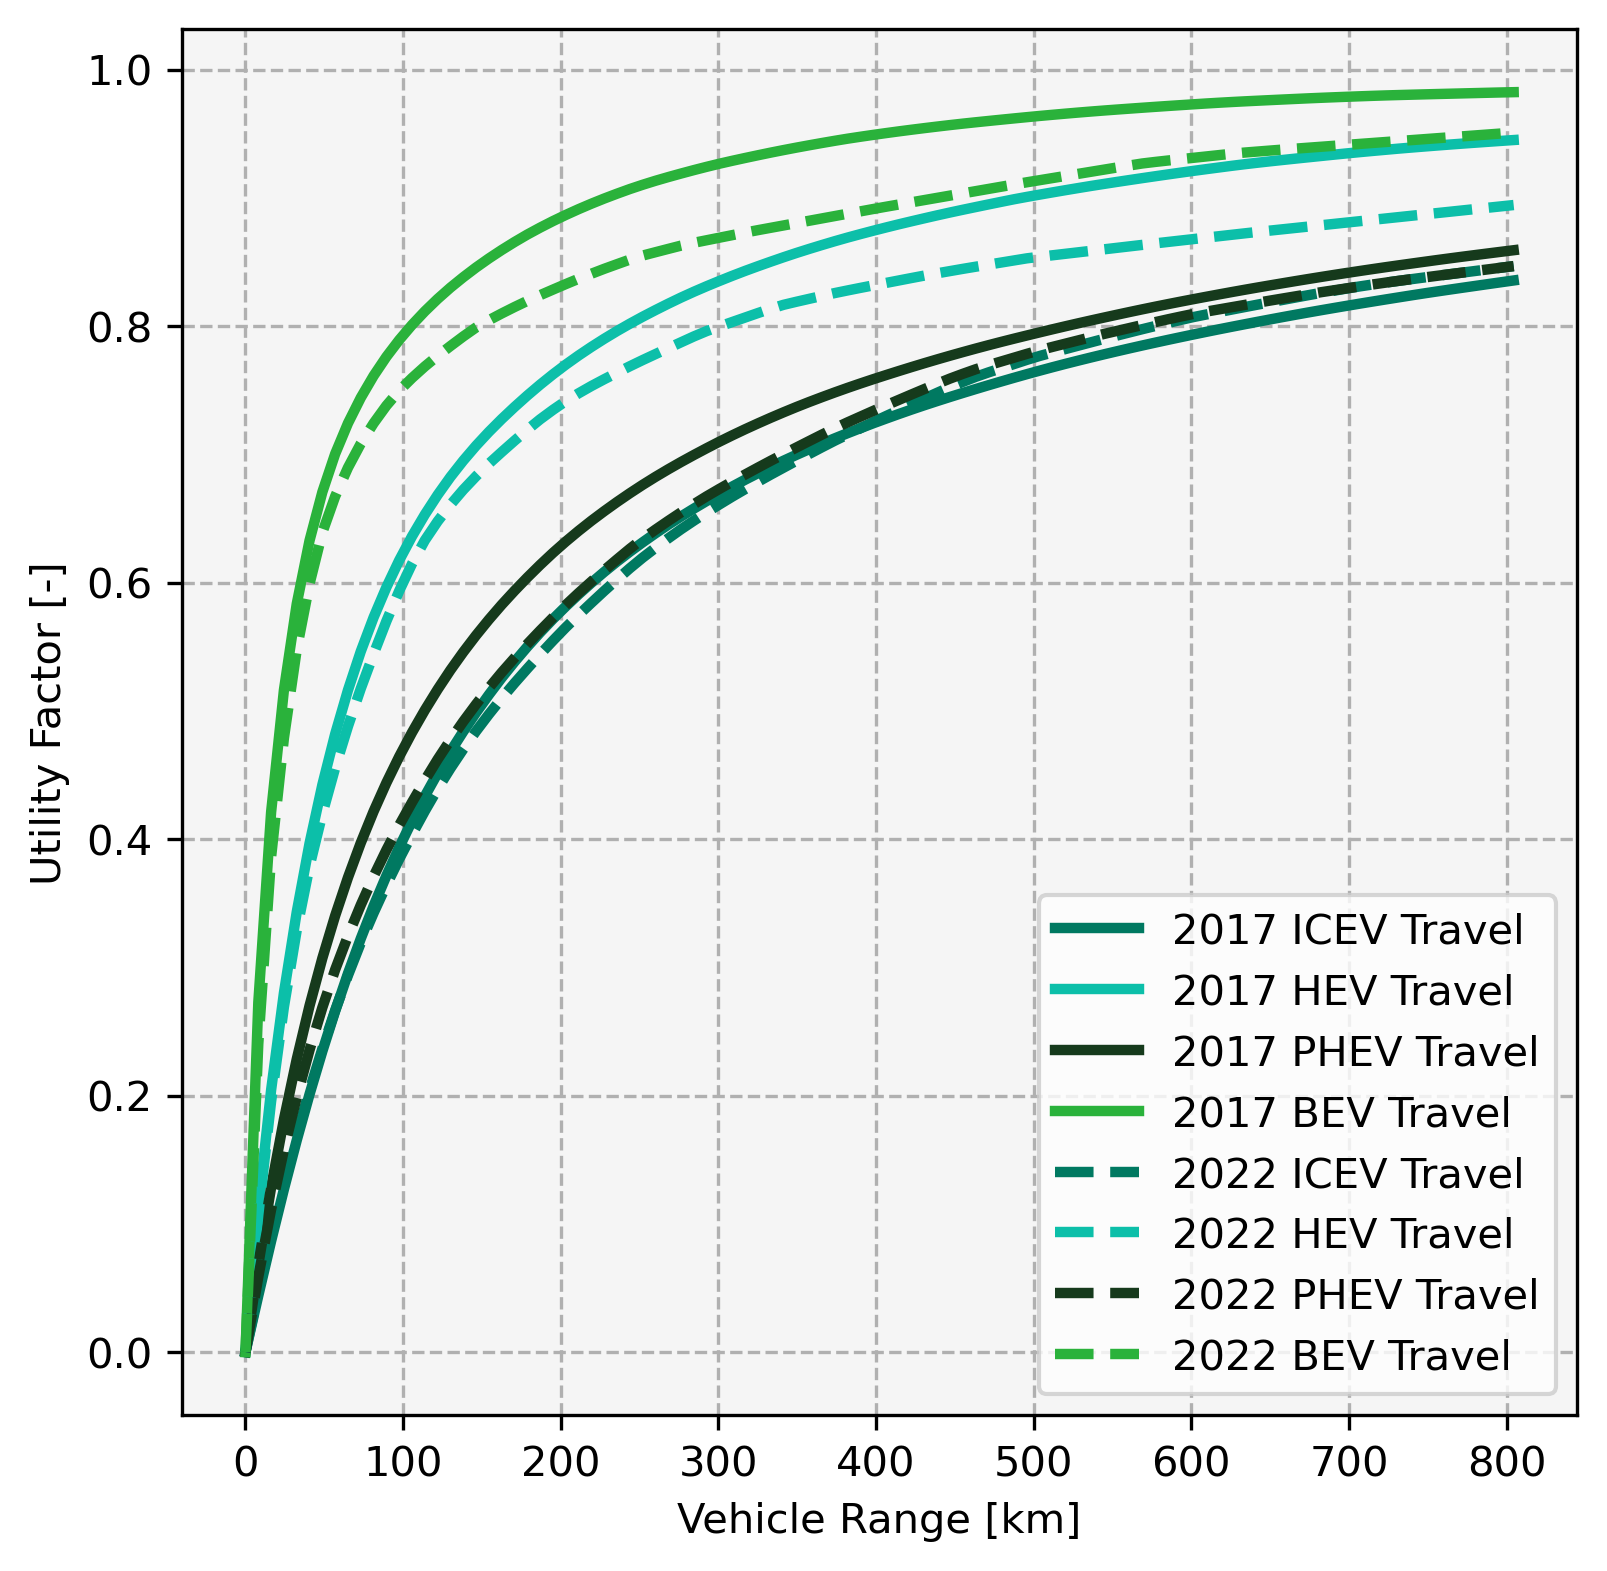
\includegraphics[width = \linewidth]{figs/UF_2017_2022_km.png}
	\caption{Individual vehicle routine travel utility factors as a function of range by powertrain type for \gls{nhts} 2017 and 2022 editions.}
	\label{fig:utility_factors}
\end{figure}

Disparities between the fueling and DC charging networks result from differences in their economic models. Gas pumping equipment requires lower up-front costs than DC \gls{evse}, is cheaper to operate \cite{Gamage_2023}, and has been deployed for far longer. Gas is often sold at low margin with stations making most profit on convenience items. Nearly all light-duty \gls{icev} drivers source all of their fuel from public fueling stations regardless of travel behavior. \gls{bev} drivers are expected to, and currently do, source much of their electricity from AC supply equipment during long dwells, often at private chargers \cite{Hardman_2018}. Thus DC charging stations are subject to higher capital expenditure, lower revenue potential, and less accumulated investment. To overcome these disadvantages, public investments in DC charging infrastructure must be made judiciously. Evaluation methods for potential charging stations should consider their network-wide impact on accessibility considering vehicle types, equipment reliability, and driver risk attitudes.

This study introduces a novel methodology to assess transportation accessibility for long vehicular trips. The methodology measures accessibility by computing optimal-feasible travel routes for \gls{od} pairs using a stochastic routing algorithm subject to vehicle range limitations, supply infrastructure, and driver risk attitudes. This methodology is powertrain agnostic and can be used to directly compare accessibility for vehicles with different ranges and which rely on different supply networks. Additionally, a case study is presented for the state of California showing a comparison between \glspl{icev} and \glspl{bev} access for important \gls{od} pairs within the state. The methodology introduced, as well as the open-source code provided in the supplemental information is a valuable tool for planners and policymakers in originating and evaluating \gls{evse} deployment policies.

\section*{Transportation Accessibility}

Transportation accessibility has been studied as a tool for urban and regional planners since the middle of the 20\textsuperscript{th} century. Accessibility derives from the theory of population migration proposed by Ravenstein in 1885 \cite{Ravenstein_1885}. The movement of populations over a given time-scale can be analogized to DC power flow. In this analogy push and pull factors determine the "voltage" separation, traversal difficulty is the "resistance" and the resulting "current" is the flow. The field of transportation accessibility uses this framework to study regional efficiency considering both voltage and resistance simultaneously. The accepted definition of transportation accessibility is the ease with which individuals can access relevant opportunities subject to the transportation system in the relevant area. Thus, accessibility is a framework which encompasses voltage factors such as land use and temporal availability, resistance factors such as transportation system design, and universal factors such as personal preference \cite{Geurs_2004}. Literature provides four essential frameworks for computing access as surveyed in \cite{Handy_1997, Kwan_1998, Geurs_2004, Miller_2018, Handy_2020} and discussed below.

Much of the difference between methodologies is in the selection of opportunities. Individuals are assumed to need or desire location-specific opportunities such as employment and physical retail. However, there may be several near-equivalents for any given opportunity type. The simplest methods for selecting opportunities are based on nearest proximity \cite{Wachs_1973, Vickerman_1974}. Proximity methods consider that a person has a level of access to a given need as determined by that person's proximity to the closest relevant opportunity. These methods do not account for heterogeneity within an opportunity category nor for the benefits of redundancy within an opportunity category. The inverse are isocost methods wherein a person is said to have access as determined by the number of opportunities available within a given isocost polygon. This method has the drawback of not considering the differences in edge traversal cost for \gls{od} pairs within the isocost region. These methods have been used widely \cite{Easa_1993} due to their computational lightness and form the basis for modern big-data methods such as the US DOE's Mobility Energy Productivity metric \cite{Hou_2019}.

Proximity and isocost methods are easy to compute because they treat redundancy arbitrarily. In practice, equivalent and near-equivalent opportunities compete with one-another if sufficiently proximate or if the paths required to reach them overlap \cite{Stouffer_1940}. Gravity/entropy methods \cite{Noulas_2012, Jung_2008} address this shortcoming. These methods are so called as they concern the cumulative effect of opportunities for a given origin on the basis of demand over proximity (gravity) or information content (entropy). Such methods were first formalized into a quantitative framework in 1959 \cite{Hansen_1959} as a generalization of previous methodology for quantifying the efficiency of urban land use. Gravity/entropy methods define accessibility as the intensity of the possibility for interaction. Implicit in the formulation of gravity/entropy methods is that every opportunity has some effect on every individual, even if negligible, and the effect of any one opportunity is determined by its network position.

Proximity and gravity/entropy methods rely on the assumption that traversal cost is the primary factor determining individuals decision to select one opportunity from among a set of similar entities. While this is certainly true if the difference in traversal cost is large enough it is not, altogether, obvious what the threshold of disambiguation is for a given individual. Thus, researchers have proposed to use Discrete Choice Modeling \cite{Ben_Akiva_1985} to explain revealed choices wherein ease-of-access is one of several possible factors in determining the utility of a given opportunity for an individual \cite{Cevero_1995, Shen_1998, Karst_2003}.

There are, thus, a variety of methods which can be used to quantify the accessibility of a given region with varying computational and data requirements. The relationship between land-use, transportation, and demography is circular rather than linear. Which method one chooses for an analysis reflects the scope and purpose of that analysis. Definition of scope can be difficult and can lead to self-defeating policies \cite{Handy_1996}. This study is concerned with the effects of electrification on long-trip accessibility for road vehicle users. This scope simplifies opportunity selection. It is necessary that a transportation system provide for access between large population centers within a region of interest and to those in adjacent regions.  This study is focused on non-routine regional travel rather than routine local travel as this is where supply infrastructure becomes important. It should be noted that the method is valid for all travel scales. Methodology is developed in the following section.

\section*{Methods}

The focus of this study is long-trip accessibility for road vehicles. The metric proposed is of the Proximity type and reflects the ease with which a given individual, driving a given vehicle, can access the important locations in a region from one-another. The metric is titled Road-trip Accessibility. It is assumed that travelers, when considering non-routine long trips have a specific destination in mind and would not consider nearly equivalent and/or equidistant locations as fungible. Rather, having determined to travel to a given location the traveler will then select a mode. Road-trip Accessibility is computed by calculating the mode and person specific lowest-cost-paths for all pairs of selected locations within the region and taking the average. Example costs which might be used are travel time and travel price. This paper will focus, exclusively, on travel time. The manner in which lowest-cost-paths are calculated is critical in arriving at a representative result. This study calls for a specific method of stochastic route optimization and evaluation which will be detailed in the subsections below.

A transportation accessibility metric should have land-use, transportation, temporal, and individual components \cite{Karst_2003}. Road-trip Accessibility contains all of these components. The land-use within a region has two principle effects on Road-trip Accessibility. First, for a multi-city region, peripheral cities should experience worse regional access than central cities. Second, geographically large and/or sparse regions should experience worse overall accessibility than compact regions. The transportation infrastructure determines the efficacy of various modes. Where only vehicular travel is concerned, the mode choice is reduced to vehicle choice. Vehicle specific infrastructure is not necessarily the same for all vehicles of a given fuel type but is necessarily different between fuel types creating effectively separate modes. The temporal component of Road-trip Accessibility arises from the schedules of public transportation services and road traffic patterns. Finally the individual component is the traveler risk attitude and route cost weights.

\subsection*{Road-trip Accessibility Metric Definition}

For region $R$ with a set of $N$ selected locations $O = \{O_1, O_2, \dots, O_N\}$ and a corresponding set of importance weights $W = \{W_0, W_1, \dots, W_N\}$, the Road-trip Accessibility metric $A_{rt}$ is

\begin{equation}
	A_{rt} = \frac{1}{N^2}\sum_{i = 0}^{N} \sum_{j = 0 }^{N} W_iW_jC(O_i, O_j) \label{eq:a_rt}
\end{equation}

\noindent where $C(O_i, O_j) $ is the cost of the optimal path from $O_i$ to $O_j$. The specific accessibility metric $A_{rt,i}$ can be computed for region $R$ and origin $i$ as

\begin{equation}
	A_{rt,i} = \frac{1}{N}\sum_{j = 0 }^{N} W_iW_jC(O_i, O_j) \label{eq:a_rt_i}
\end{equation}

for any origin $O_i \in O$. Road-trip Accessibility is a weighted mean of costs to access important locations from either a specific location or for all-pairs. The all-pairs implementation \eqref{eq:a_rt} is titled General Road-trip Accessibility while the single-origin implementation \eqref{eq:a_rt_i} is titled Specific Road-trip Accessibility. A given score applies to a given region, travel mode, and individual person. Comparisons may be made between different combinations by computing scores for each combination.

\subsection*{Computing the Road-trip Accessibility Metric}

Powered vehicles are range-limited due to the finite capacity of their \glspl{ess}. In order to traverse an \gls{od} arc whose energy requirement is greater than a given limit, a vehicle must stop at a supply station. In practical terms, the limit is defined by the vehicle's \gls{ess} capacity, starting \gls{soc}, desired finishing \gls{soc}, and the driver's low \gls{soc} tolerance. Because supply events add time to a trip, they will usually be avoided on short trips. For sufficiently long trips, where at least one supply event is necessary, computing the lowest-cost-path requires considering the time added by supply events and the locations of supply stations. These are, usually, not considered as, for \glspl{icev}, supply events are brief and supply stations are ubiquitous in most areas of the developed world. However, for \glspl{bev}, where supply events are lengthy and where DC supply stations are comparatively rare, ignoring supply events when computing a lowest-cost-path carries non-negligible risk. For this reason, dedicated \gls{bev} routing services compute routes considering supply events [SOURCE  - a better route planner].

A further complication is that the driver will have limited and uncertain information with which to evaluate alternatives at the beginning of the trip. Variables such as traffic, temporary road closures, supply equipment non-functionality, and queues at supply stations cannot be precisely known at the start of a trip. The ability to estimate delays and the severity of delays vary among the previously mentioned events. As the driver progresses, certainty may increase but factors such as charger availability may change up to the instant that the driver arrives at the charger. As such, the driver will have to plan to optimize the expected result. This is replicated via stochastic optimization.

\subsubsection*{Stochastic Optimal Routing}

The purpose of stochastic optimal routing is to find the expected lowest-cost-paths from a given origin $i \in V$ to a set of destinations $D \in V$ on a graph $G = \{V, E\}$. The output is tree $P$ containing the optimal-feasible paths from the origin to the selected destinations. The objective of routing between nodes $i$ and $j\in D$ is

\begin{equation}
	\min_{U \in \overline({U}_{i,j})}\ \mathbb{E}[J(S_0, U)]
\end{equation}

where

\begin{equation}
	J(U) = \sum_{k = 0}^M \Phi_k(S_0, U)
\end{equation}

s.t.

\begin{gather}	
	b^k_l \leq \mathbb{E}\left[\int_0^t \Phi_k(S_0, U)dt\right] \leq b^k_u\\
	\mathbb{E}\left[\int_0^T \Phi_k(S_0, U)dt\right] \geq b^k_f\\
	 t \in [0, T]\quad k = 1, 2, \dots, M
\end{gather}

\noindent where $T$ is the final value of time for a route, $S$ is the state vector, $S_0$ is the initial values of the states, $U$ is a control (route) between $i$ and $j$, $\overline{U}_{i,j}$ is the set of possible routes between $i$, and $j$, $\Phi$ is the set of cost functions, $b^k_l$ and $b^k_u$ are the upper and lower bounds for state $k$ respectively, and $b^k_f$ is the final state minimum value for state $k$. $\mathbb{E}$ denotes an expectation. State vector $S$ is initialized and stored as vectors containing $N$ discreet variables. A distribution $D$ for a the state vector at any node and time-step can be computed from a histogram of the values. States can be changed at nodes and edges. Routes are considered feasible if state expectations remain within set bounds. Comparison between routes is performed using cost expectation. Routing depends on vehicle, infrastructural, and individual models.


\subsubsection*{Vehicle Model}

Vehicles effect routing due to their range limits and supply methods. The vehicle model used herein is highly simplified due to the inexact nature of the problem. Vehicles serve to store energy and consume energy at a constant rate per unit distance driven. More exact information on road conditions, traffic conditions, and atmospheric conditions among others can be used to compute edge-specific efficiencies. Vehicular parameters are listed in Table \ref{tab:param_veh}.

\begin{table}[H]
	\centering
	\caption{Vehicle Parameters for Routing}
	\label{tab:param_veh}
	\begin{tabular}{|C{\linewidth*3/8}|C{\linewidth*3/8}|C{\linewidth*2/8}|}
		\hline Parameter & Description & Unit \\
		\hline \gls{ess} Capacity & Accessible energy storage capacity & [kWh] \\
		\hline Energy Consumption & Energy required to move the vehicle & [kJ/km] \\
		\hline Supply Rate & \gls{ess} maximum energy addition rate & [kW] \\
		\hline Supply Limits & \gls{soc} bounds for supply & [-] \\
		\hline
	\end{tabular}
\end{table}

\subsubsection*{Supply Infrastructure Network Model}

Supply networks effect routing both in structure and in the characteristics of individual stations. In this paper, the supply network refers to all stations which the vehicle can utilize rather than the industry definition which covers stations operated by a single \gls{cpo}. Networks ultimately consist of individual supply ports (chargers or fuel pumps) and serve large and geographically distributed demand. A network consisting of more than one port can develop redundancy either by concentrating ports in a single confined space "in-station" or via a more evenly distributed approach "between-station". Network redundancy also varies by location with "thinner" and "thicker" coverage areas.

Vehicle optimal routing serves to find the lowest-cost-path between two points on a road atlas atlas. A road atlas is a graph with a large number of nodes and a low edge-to-node ratio. When considering a multi-leg itinerary, such as when solving the Traveling Salesman Problem or Vehicle Routing Problem, the atlas need not be stored in entirety. Only the locations of and relationships between relevant nodes are necessary. The graph formed from the relevant nodes and their relationships is a reduced subgraph with a low number of nodes and relatively high edges-per-node and cycles-per-node ratios. A reduced subgraph is defined as follows. For a graph $G = \{V, E\}$ where $V$ is the set of nodes and $E$ is the set of edges, a reduced subgraph $\hat{G} = \{\hat{V}, \hat{E}\}$ can be computed where $\hat{V} \subseteq V$ and $\hat{E}$ is the set of shortest-paths between all nodes in $\hat{V}$. An example of a reduced subgraph is shown in Figure \ref{fig:reduced_subgraph}.

\begin{figure}[H]
	\centering
	\begin{subfigure}[t]{.5\linewidth}
		\centering\captionsetup{width = .8\linewidth}
		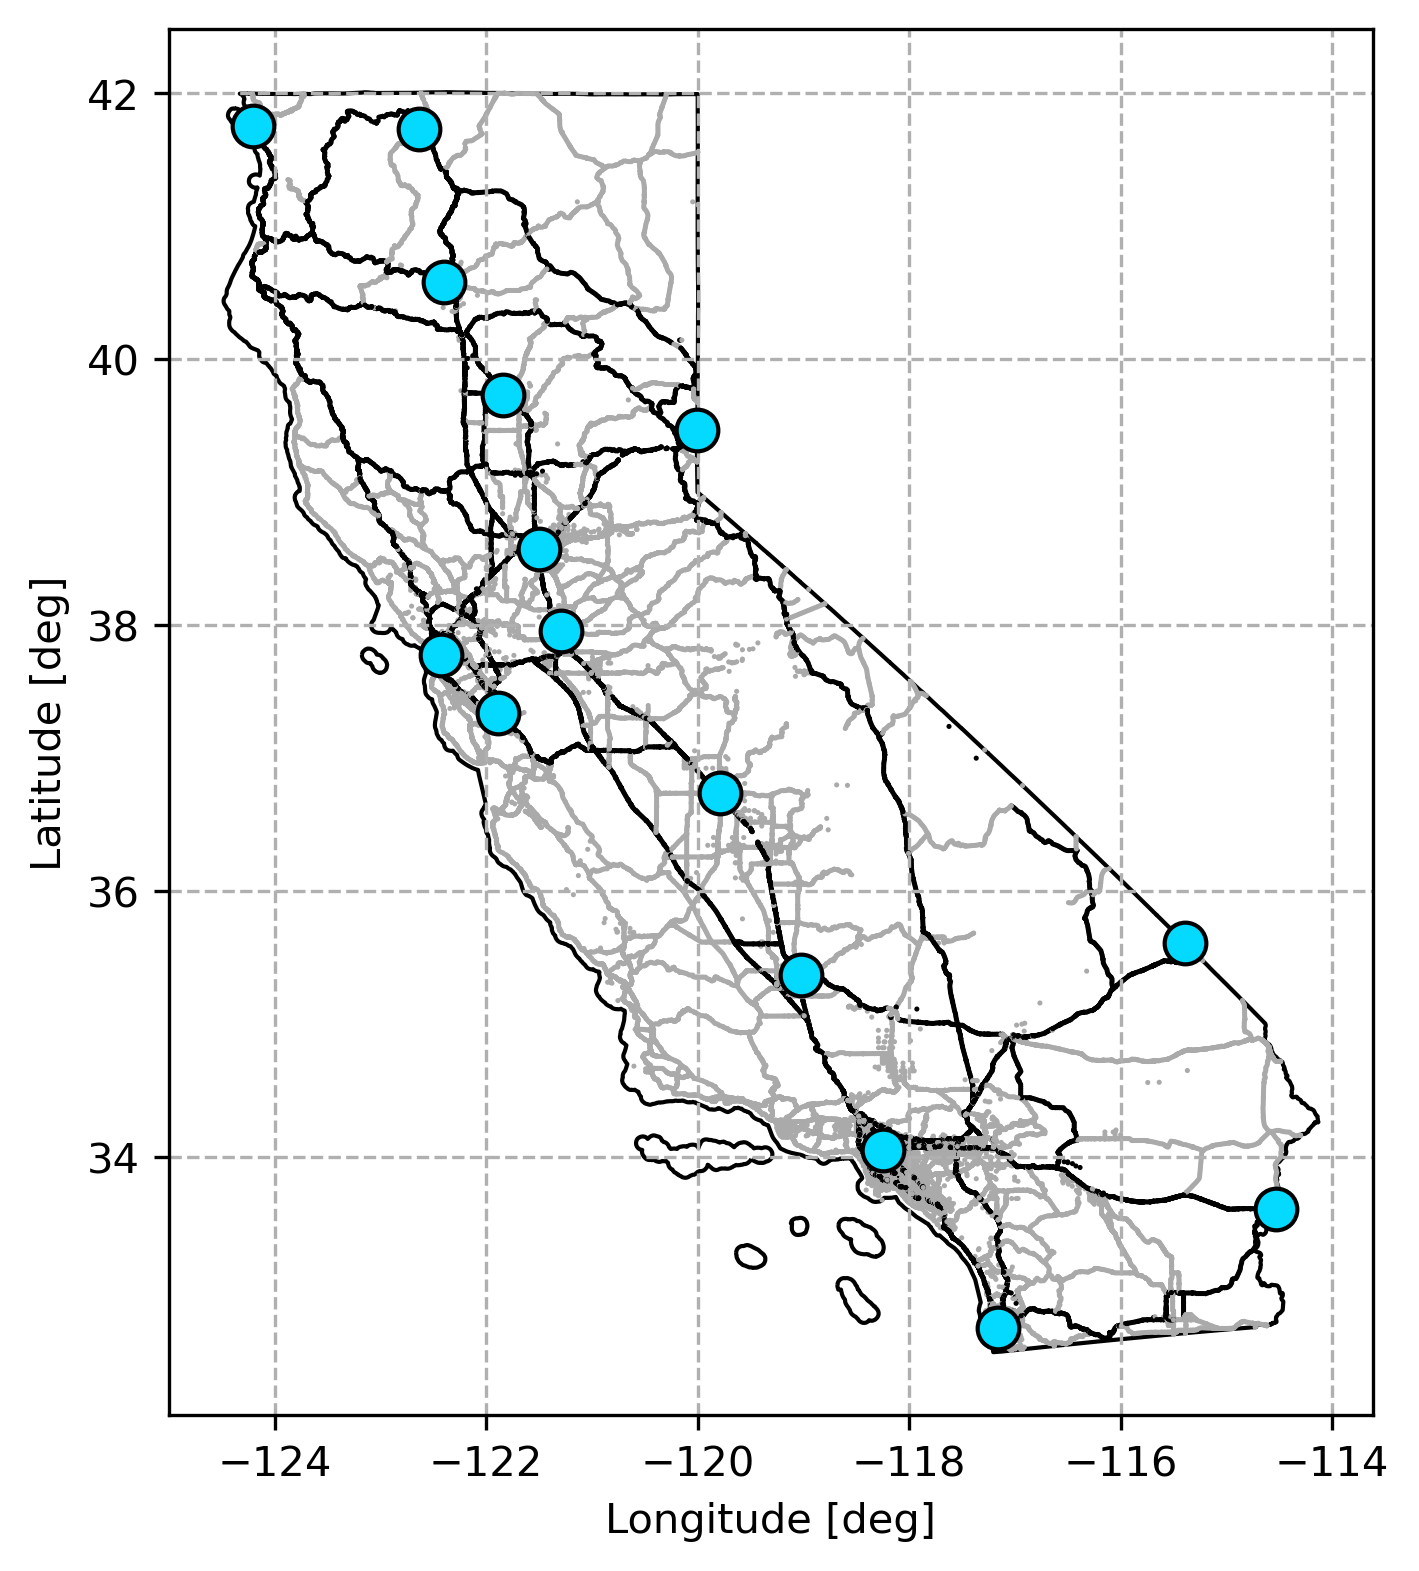
\includegraphics[width = \linewidth]{figs/full_graph.png}
%		\caption{Locations and routes between selected nodes on atlas}
	\end{subfigure}%
	\begin{subfigure}[t]{.5\linewidth}
		\centering\captionsetup{width = .8\linewidth}
		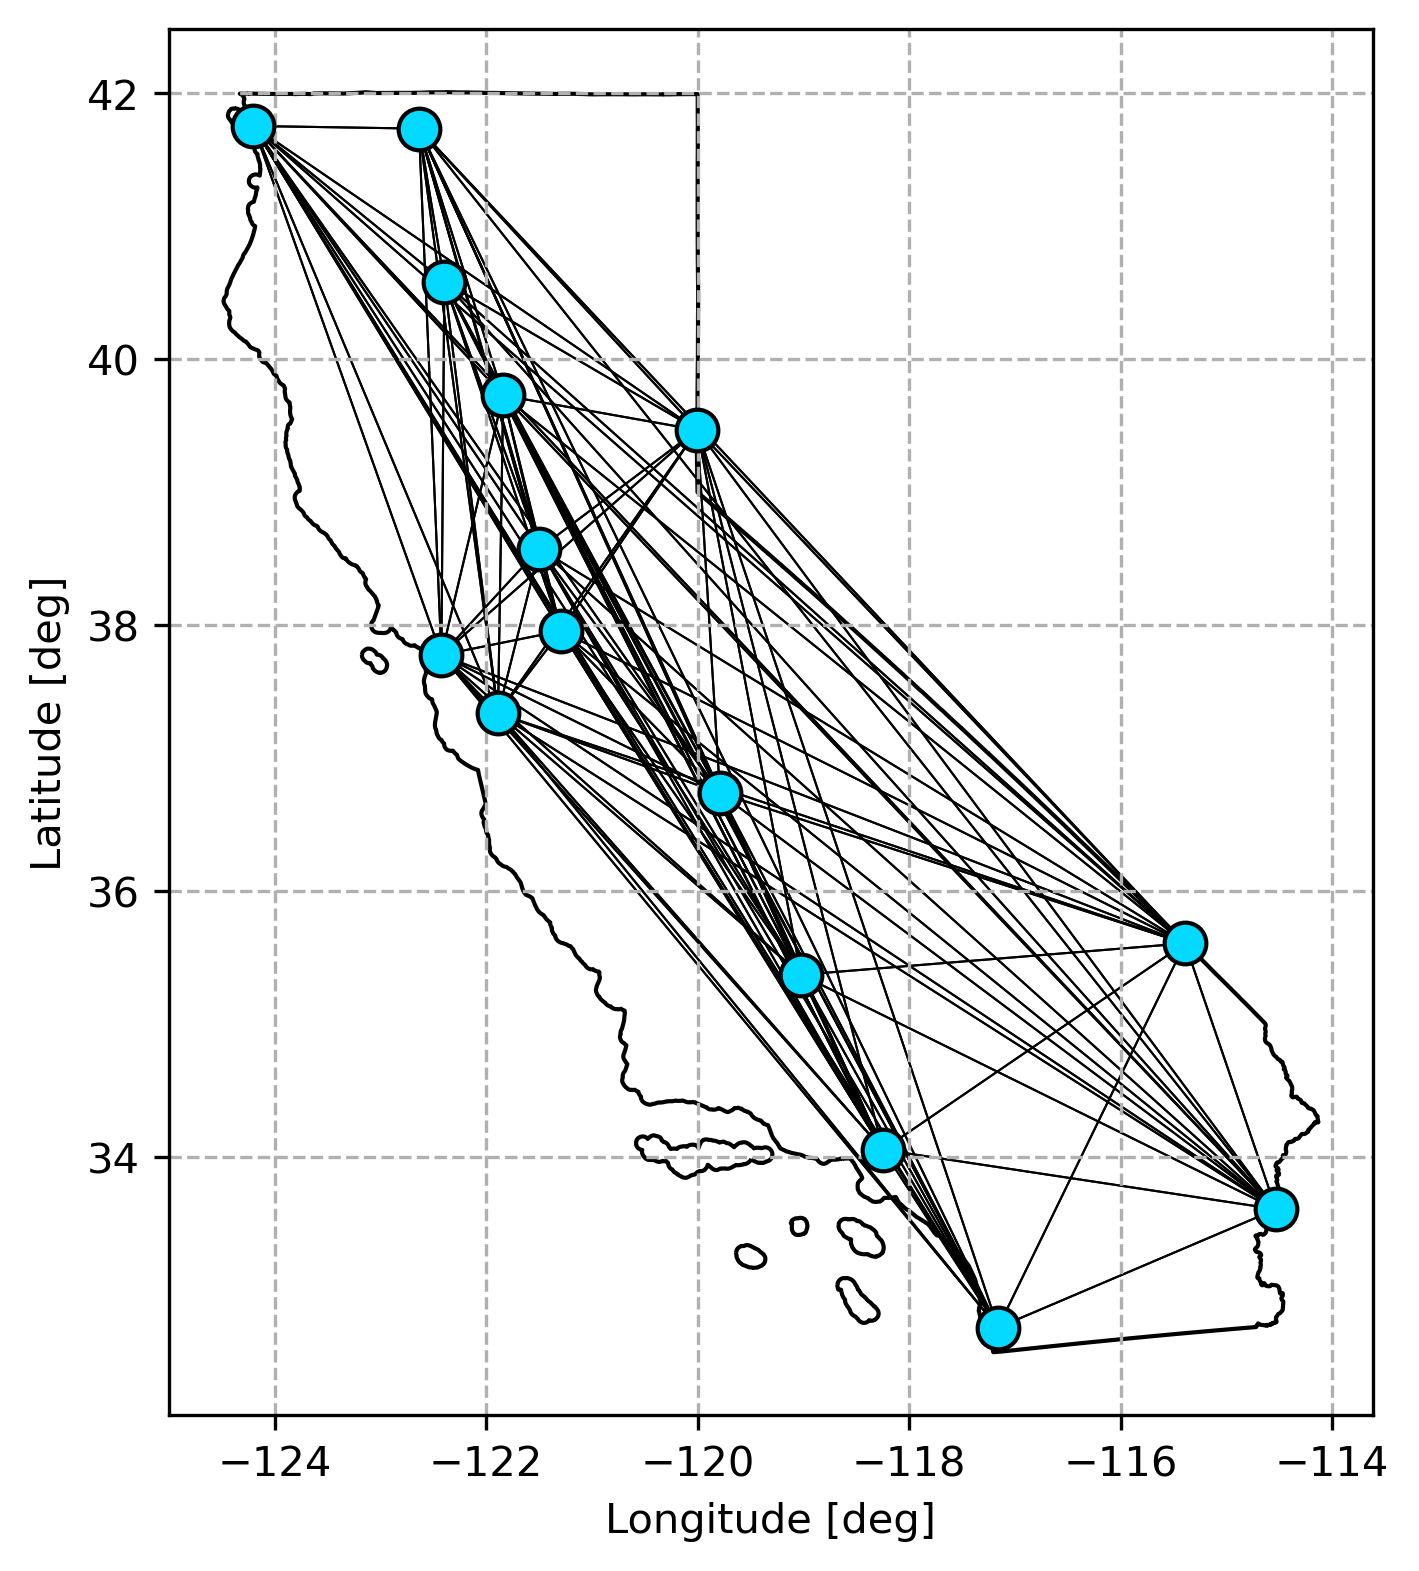
\includegraphics[width = \linewidth]{figs/reduced_graph.png}
%		\caption{Reduced graph containing locations of and relationships between selected nodes}
	\end{subfigure}
	\caption{Example original graph (a) containing locations and an atlas and reduced subgraph (b) containing locations and arcs.}
%	The locations selected are key destinations in the state or on its border. Logistical optimization requires, first computing arcs between \gls{od} pairs as in the right pane based on the atlas in the left pane.}
	\label{fig:reduced_subgraph}
\end{figure}

For a given vehicle type, the \gls{sng} is the reduced subgraph containing the trip origin, trip destination, and all supply stations reasonably likely to be utilized. Alternatively the \gls{sng} can contain a set of origins and destinations in order to enable further reduction for logistical optimization purposes. In-station redundancy for a \gls{sng} is a node parameter. In-station $R_{is}$ redundancy for any node $v \in V$ on \gls{sng} $G = \{V, E\}$ is the number of ports at node $v$. Between-station redundancy $R_{bs}$ for an \gls{sng} is a clique parameter. Between-station redundancy for any clique $C \subseteq V$ on \gls{sng} $G = \{V, E\}$ is the sum of the ports at nodes $v \in C$. A more meaningful result for $R_{bs}$ may be returned by limiting the cost of edges considered. For example, $R'_{bs}$ may be computed for $G' = \{V, E'\}$ where $E' \subseteq E$ contains all edges of less than 10 minutes drive time.

The \gls{sng} is the graph on which long vehicle trips should be optimized if supply events are expensive and/or constraining. In general, because the road atlas will have a low cycle-to-node ratio, the Bellman algorithm will be faster while the Bellman-Ford algorithm (specifically the SPFA variant) will be faster for the \gls{sng} with its high cycle-to-node ratio. The relevant \gls{sng} for \glspl{icev} and \gls{bev} are neither equivalent nor isomorphic. Different vehicles within a given powertrain type may also have different \glspl{sng} but this is far more common for \glspl{ev} than \glspl{icev}. The \gls{sng} informs routing by providing a set of possible paths between origins and destinations. The structure of a network may make for a greater or lesser number of available paths depending on the number and location of stations.

Supply station characteristics significantly impact the expected cost of utilizing a given station. Supply stations are defined by the number of ports, the reliability of ports, the maximum supply rate of ports, the rate of user arrivals, and the durations of supply events. In combination, these factors determine the likelihood of a port being usable and available as well as the likely duration of queue if no port is usable and available. Supply station parameters are listed in Table \ref{tab:param_supply}.

\begin{table}[H]
	\centering
	\caption{Supply Station Parameters for Routing}
	\label{tab:param_supply}
	\begin{tabular}{|C{\linewidth*2/8}|C{\linewidth*3/8}|C{\linewidth*3/8}|}
		\hline Parameter & Description & Unit \\
		\hline Arrivals Ratio & Arrival rate at station per port and unit of time & [cars/port/hour] \\
		\hline Supply Rate & Maximum rate of energy supply & [kW] \\
		\hline Supply Energy & Expected energy supplied to vehicles & [kWh] \\
		\hline Ports & Number of chargers/pumps at a station which can be used simultaneously & [-] \\
		\hline Reliability & Percentage of the time that a given pump will be usable & [-] \\ 
		\hline
	\end{tabular}
\end{table}

Unfortunately, with the exception of the number of ports and the maximum supply rate, little of this information is available before arrival [SOURCE]. As a result, arrivals ratio, supply energy, and reliability must be estimated. To reflect this uncertainty, distributions are used for arrivals ratio and supply energy. Information on ports is taken from \gls{afdc} \cite{afdc_2023}, and information on chargers is taken from \cite{Rempel_2023}. The delays which result from DC charging station parameters are modeled as M/M/s queues and are demonstrated in \ref{fig:expected_delay}.

\begin{figure}[H]
	\centering
	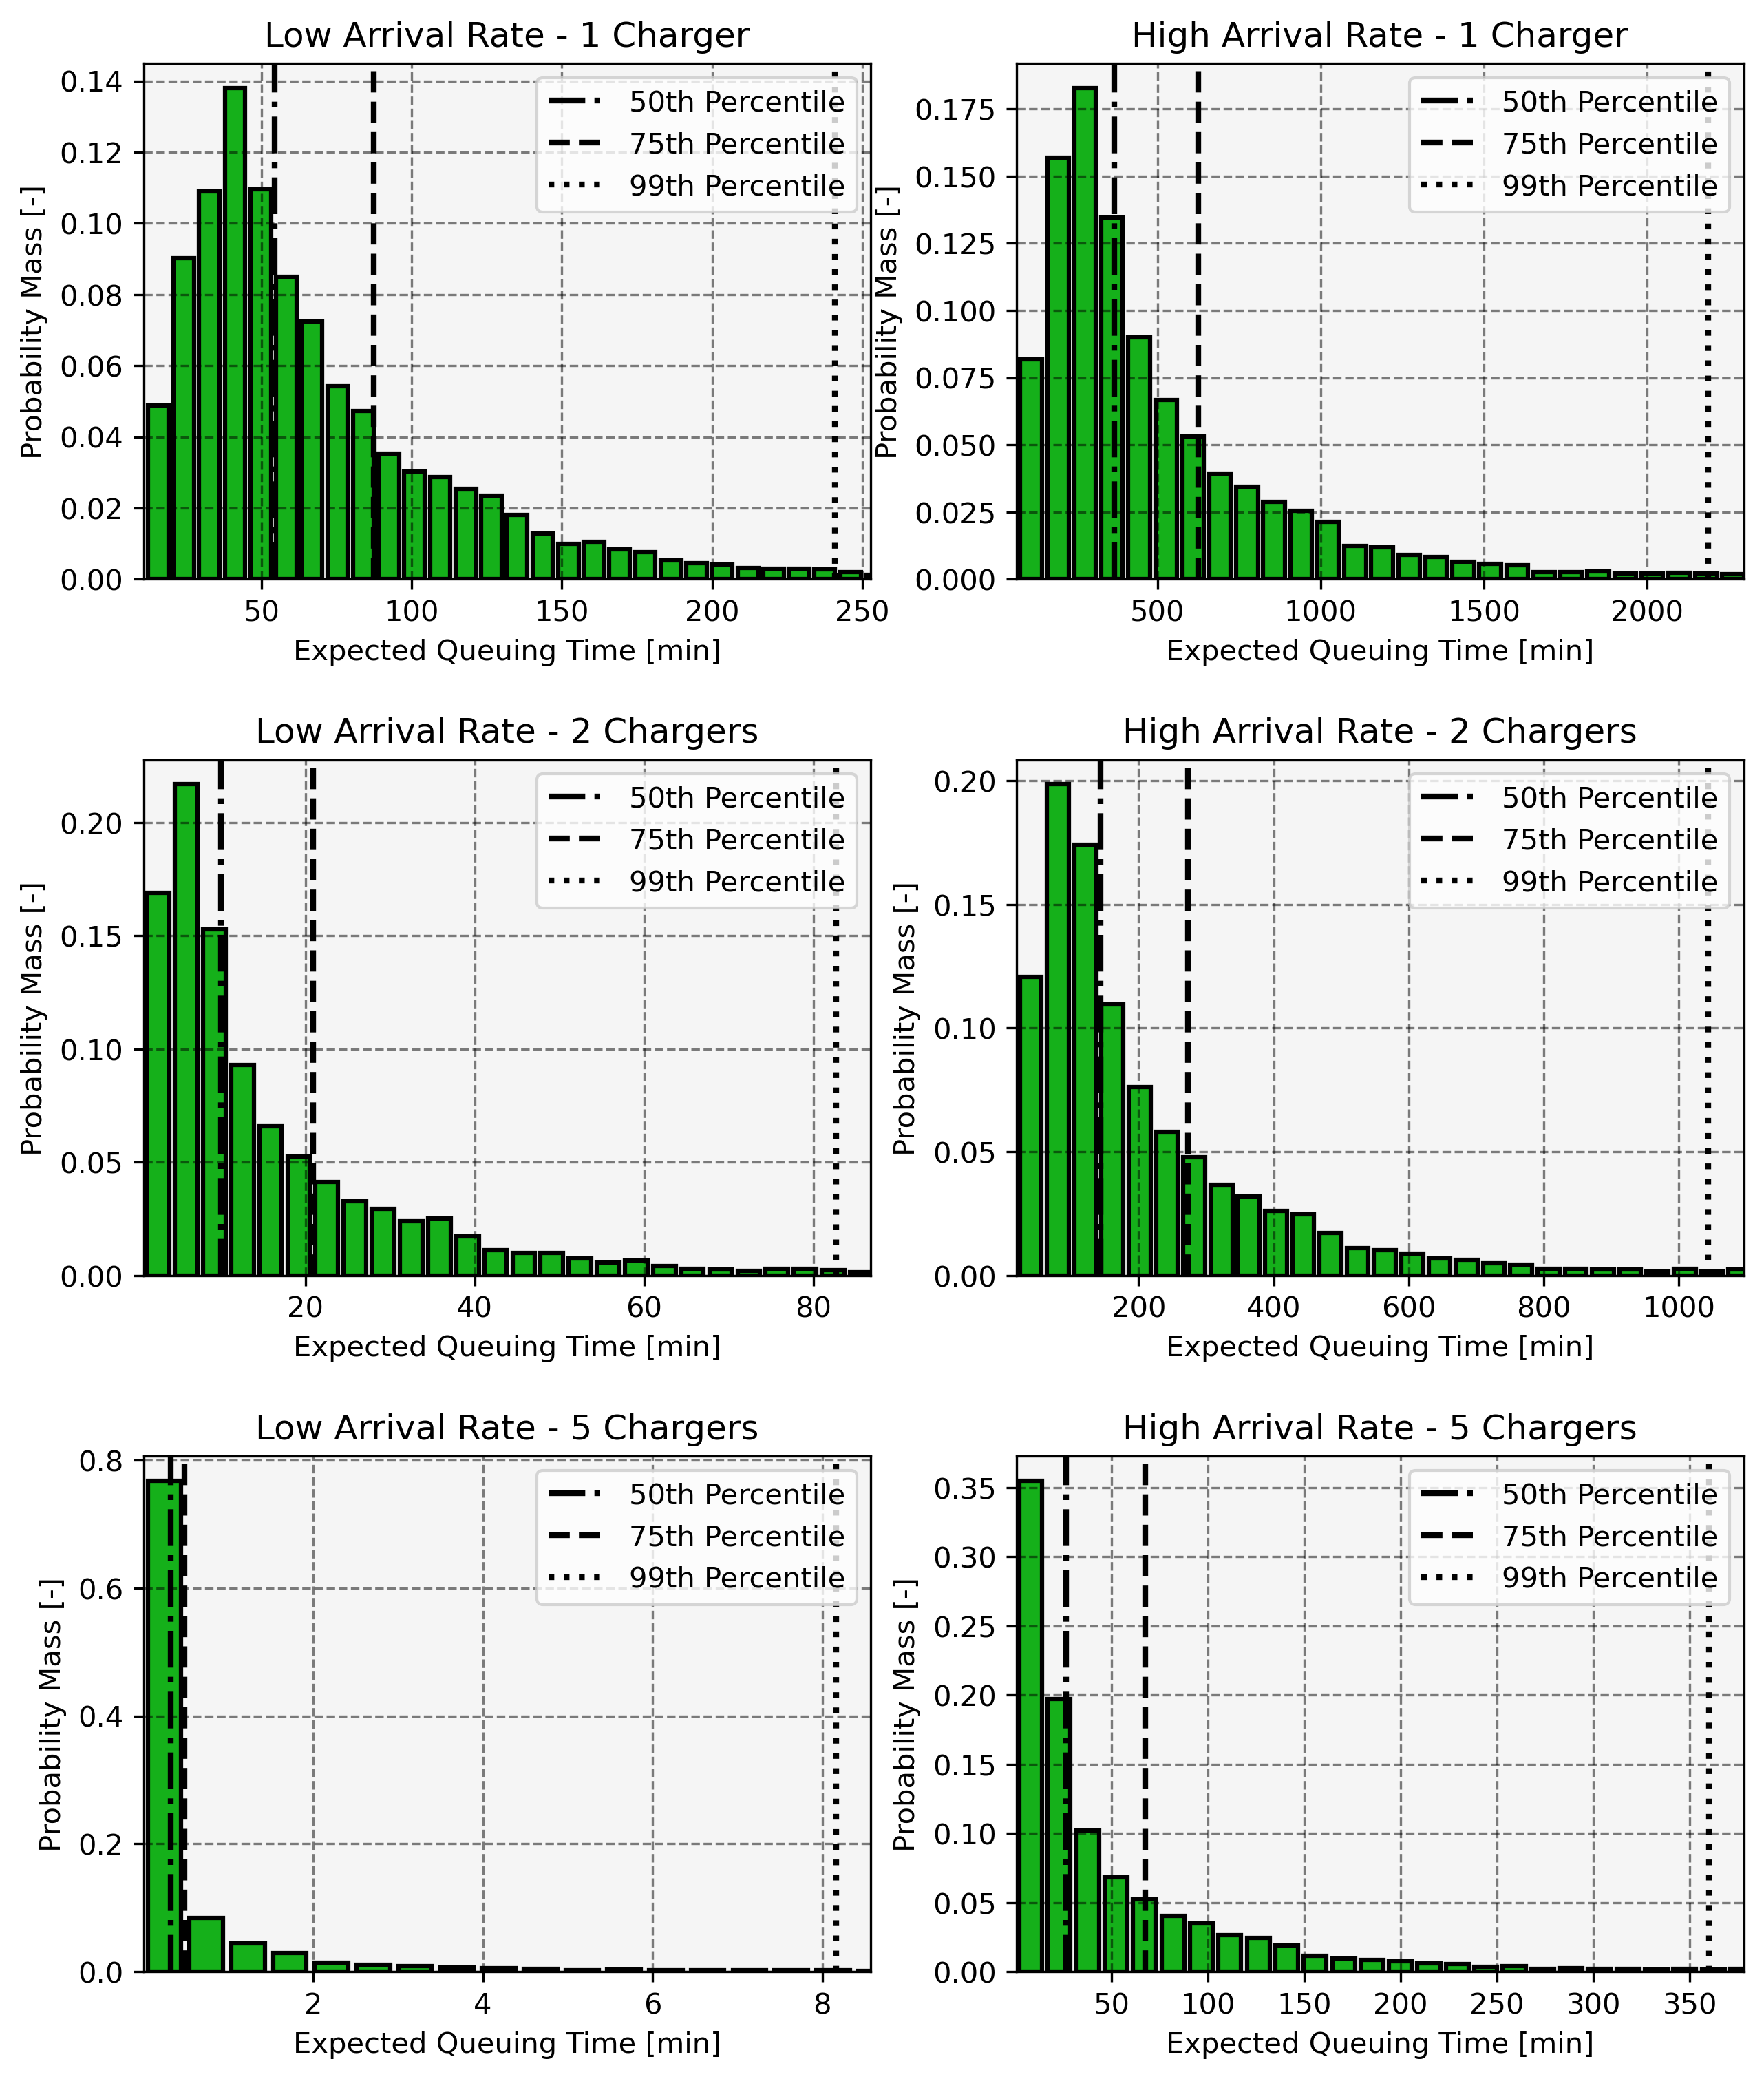
\includegraphics[width = \linewidth]{figs/expected_delay.png}
	\caption{Expected queuing time at charging stations. Low arrival rate is 10 - 60 minutes between arrivals. High arrival rate is 1 - 10 minutes between arrivals. All charge rates are 80 kW and charge events are 60 $\pm$ 15 kWh.}
	\label{fig:expected_delay}
\end{figure}

The mean arrivals rate is not known precisely, nor is the mean service rate so each is sampled from a distribution. In Figure \ref{fig:expected_delay} the columns show different distributions of arrivals rate and the rows show different levels of port redundancy. It can be observed that each factor is substantial in determining expected queue length and that their effects are additive. Without better information, a driver will have to make an educated guess as to how busy a station is likely to be and how many of its listed chargers will be functional. Getting either factor wrong could have serious consequences if the driver does not have the option to easily reach a different station where the driver may have no better information regardless. Reflecting the lack of information this study uses very broad assumptions for arrivals rate distribution and charge energy distribution. Arrivals rate is assumed to be a ratio of vehicles per hour per charger normally distributed as $N(1, 0.5)$. Charge energy delivered is assumed to be normally distributed as $N(60, 15)$ in kWh. \gls{icev} supply infrastructure is assumed to be ubiquitous with massive redundancy within and between stations such that supply requires neither deviation nor delay.

\subsubsection*{Drivers}

Given the same physical circumstances, different drivers will evaluate route costs differently. In a basic sense, drivers will weight several factors such as time, money, distance, and complexity differently. Where any important factor is not known precisely drivers will consider a range of outcomes and decide based on an expectation. Driver risk attitude concerns what range of outcomes will be used to compute expected cost. Risk attitude is modeled using a superquantile risk function defined as

\begin{equation}
	S(D, p_0, p_1) = \frac{1}{p_1 - p_0}\int_{p_0}^{p_1}Q(D, \alpha)\ d\alpha \label{eq:superquantile}
\end{equation}

\noindent where $D$ is a distribution, $p_0$ and $p_1$ are the boundaries of the range of probabilities considered in the expectation, and $Q$ is the quantile function of $D$. The superquantile is, thus, the mean value of a distributed quantity within a range of probability. $S(D, 0, 1)$ reduces to the mean of $D$. Drivers with an aggressive risk attitude will consider a low range of probabilities. Drivers with a neutral attitude will consider a central range of probabilities. Drivers with a cautious attitude will consider a high range of probabilities. Driver parameters are listed in Table \ref{tab:param_driver}.

\begin{table}[H]
	\centering
	\caption{Supply Station Parameters for Routing}
	\label{tab:param_driver}
	\begin{tabular}{|C{\linewidth*3/8}|C{\linewidth*3/8}|C{\linewidth*2/8}|}
		\hline Parameter & Description & Unit \\
		\hline Route Cost Weights $W$ & Set of multipliers for route costs to be used in computation of weighted sum & [-] \\
		\hline Probability Range $(p_0, p_1)$ & Range of probabilities for superquantile function & [-] \\
		\hline
	\end{tabular}
\end{table}

The driver model serves to bias the routing by selecting a subset of information to use in optimization. As such it reflects individual perception. The results of the routing can be interpreted through the same bias, a different bias, or no bias. Thus Road-trip accessibility can be as perceived (with bias) ot as expected (without bias). In this study, evaluation will be conducted on the basis of expectation.

\subsection*{Randomly Generated Example}

The Road-trip accessibility method and metric is demonstrated using a vehicle on a randomly generated \gls{sng}. In this example, a \gls{sng} containing 15 locations and 85 stations distributed across a 1000 km square is generated with randomized node locations. Edges exist between all nodes and are assigned Pythagorean distances. All edges are assumed to be traversed at 105 kmh. The origin is selected as Location 0 located in the lower-right corner with all other locations as destinations and a Specific Road-trip Accessibility is computed for Location 0. The vehicle used has a relatively short range of 262 km. The charging stations have between 1 and 5 chargers. Arrivals ratio and supply energy are sampled from normal distributions $N(1, 0.5)$ and $N(60, 15)$ respectively. Figure \ref{fig:perceived_srta_random} shows the times to travel to each destination as well as the path taken along the \gls{sng} under four different scenarios.

\begin{figure}[H]
	\centering
	\begin{subfigure}[t]{.5\linewidth}
		\centering\captionsetup{width = .8\linewidth}
		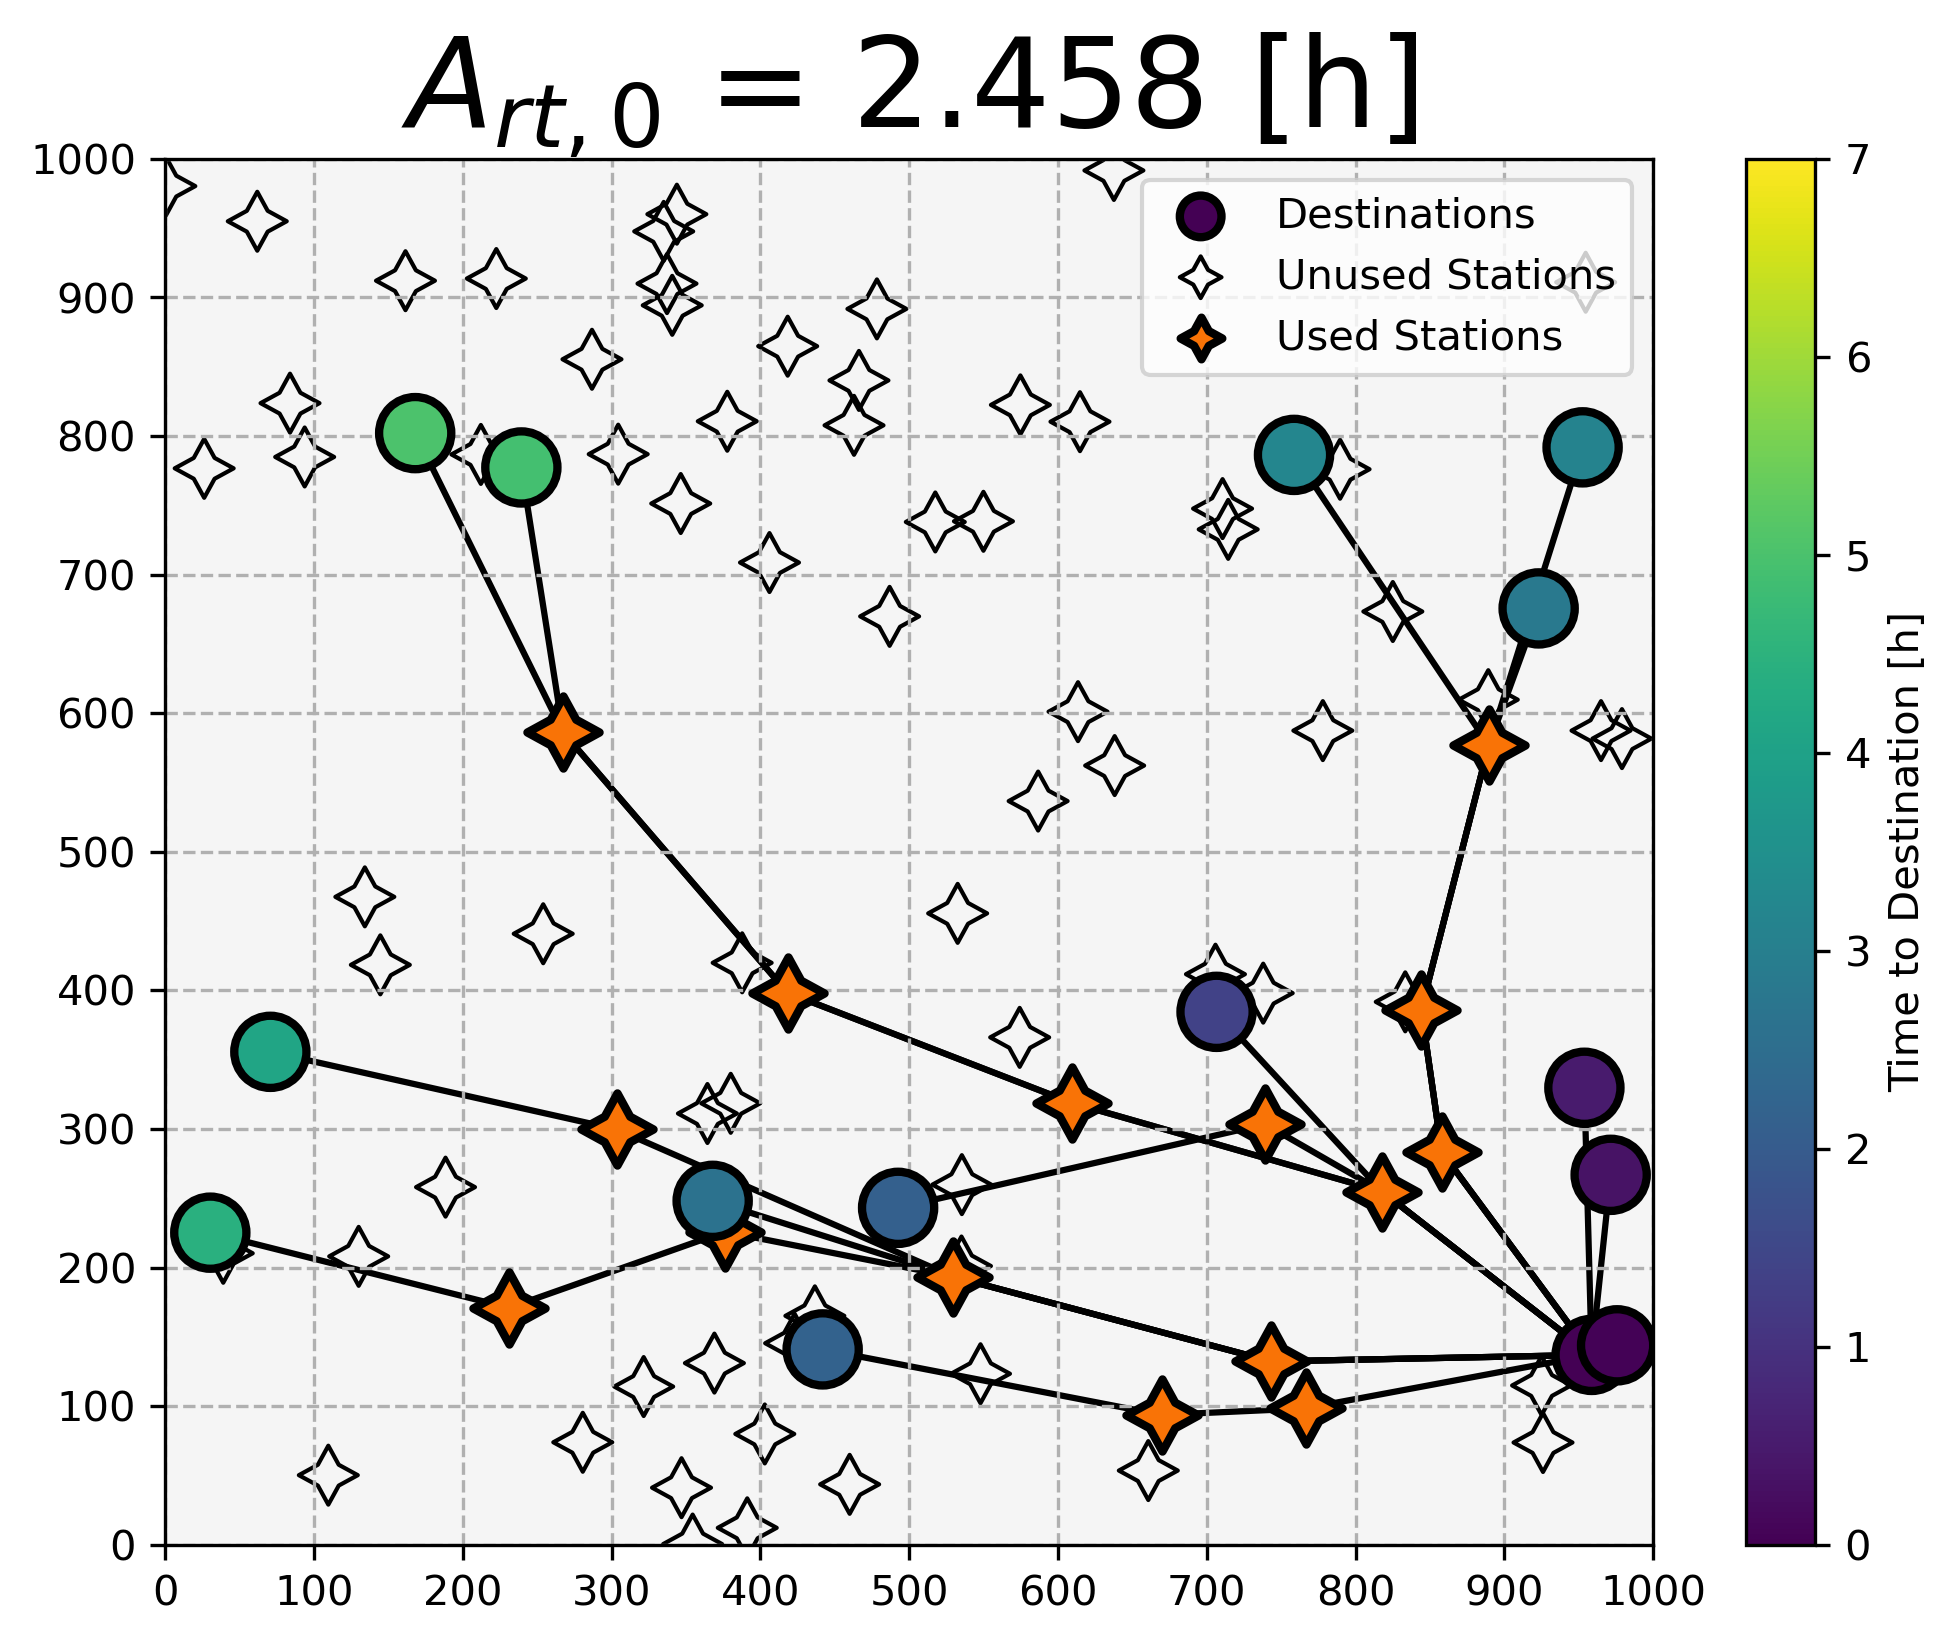
\includegraphics[width = \linewidth]{figs/random_example_high_reliability_aggressive.png}
		\caption{High reliability, aggressive}
	\end{subfigure}%
	\begin{subfigure}[t]{.5\linewidth}
		\centering\captionsetup{width = .8\linewidth}
		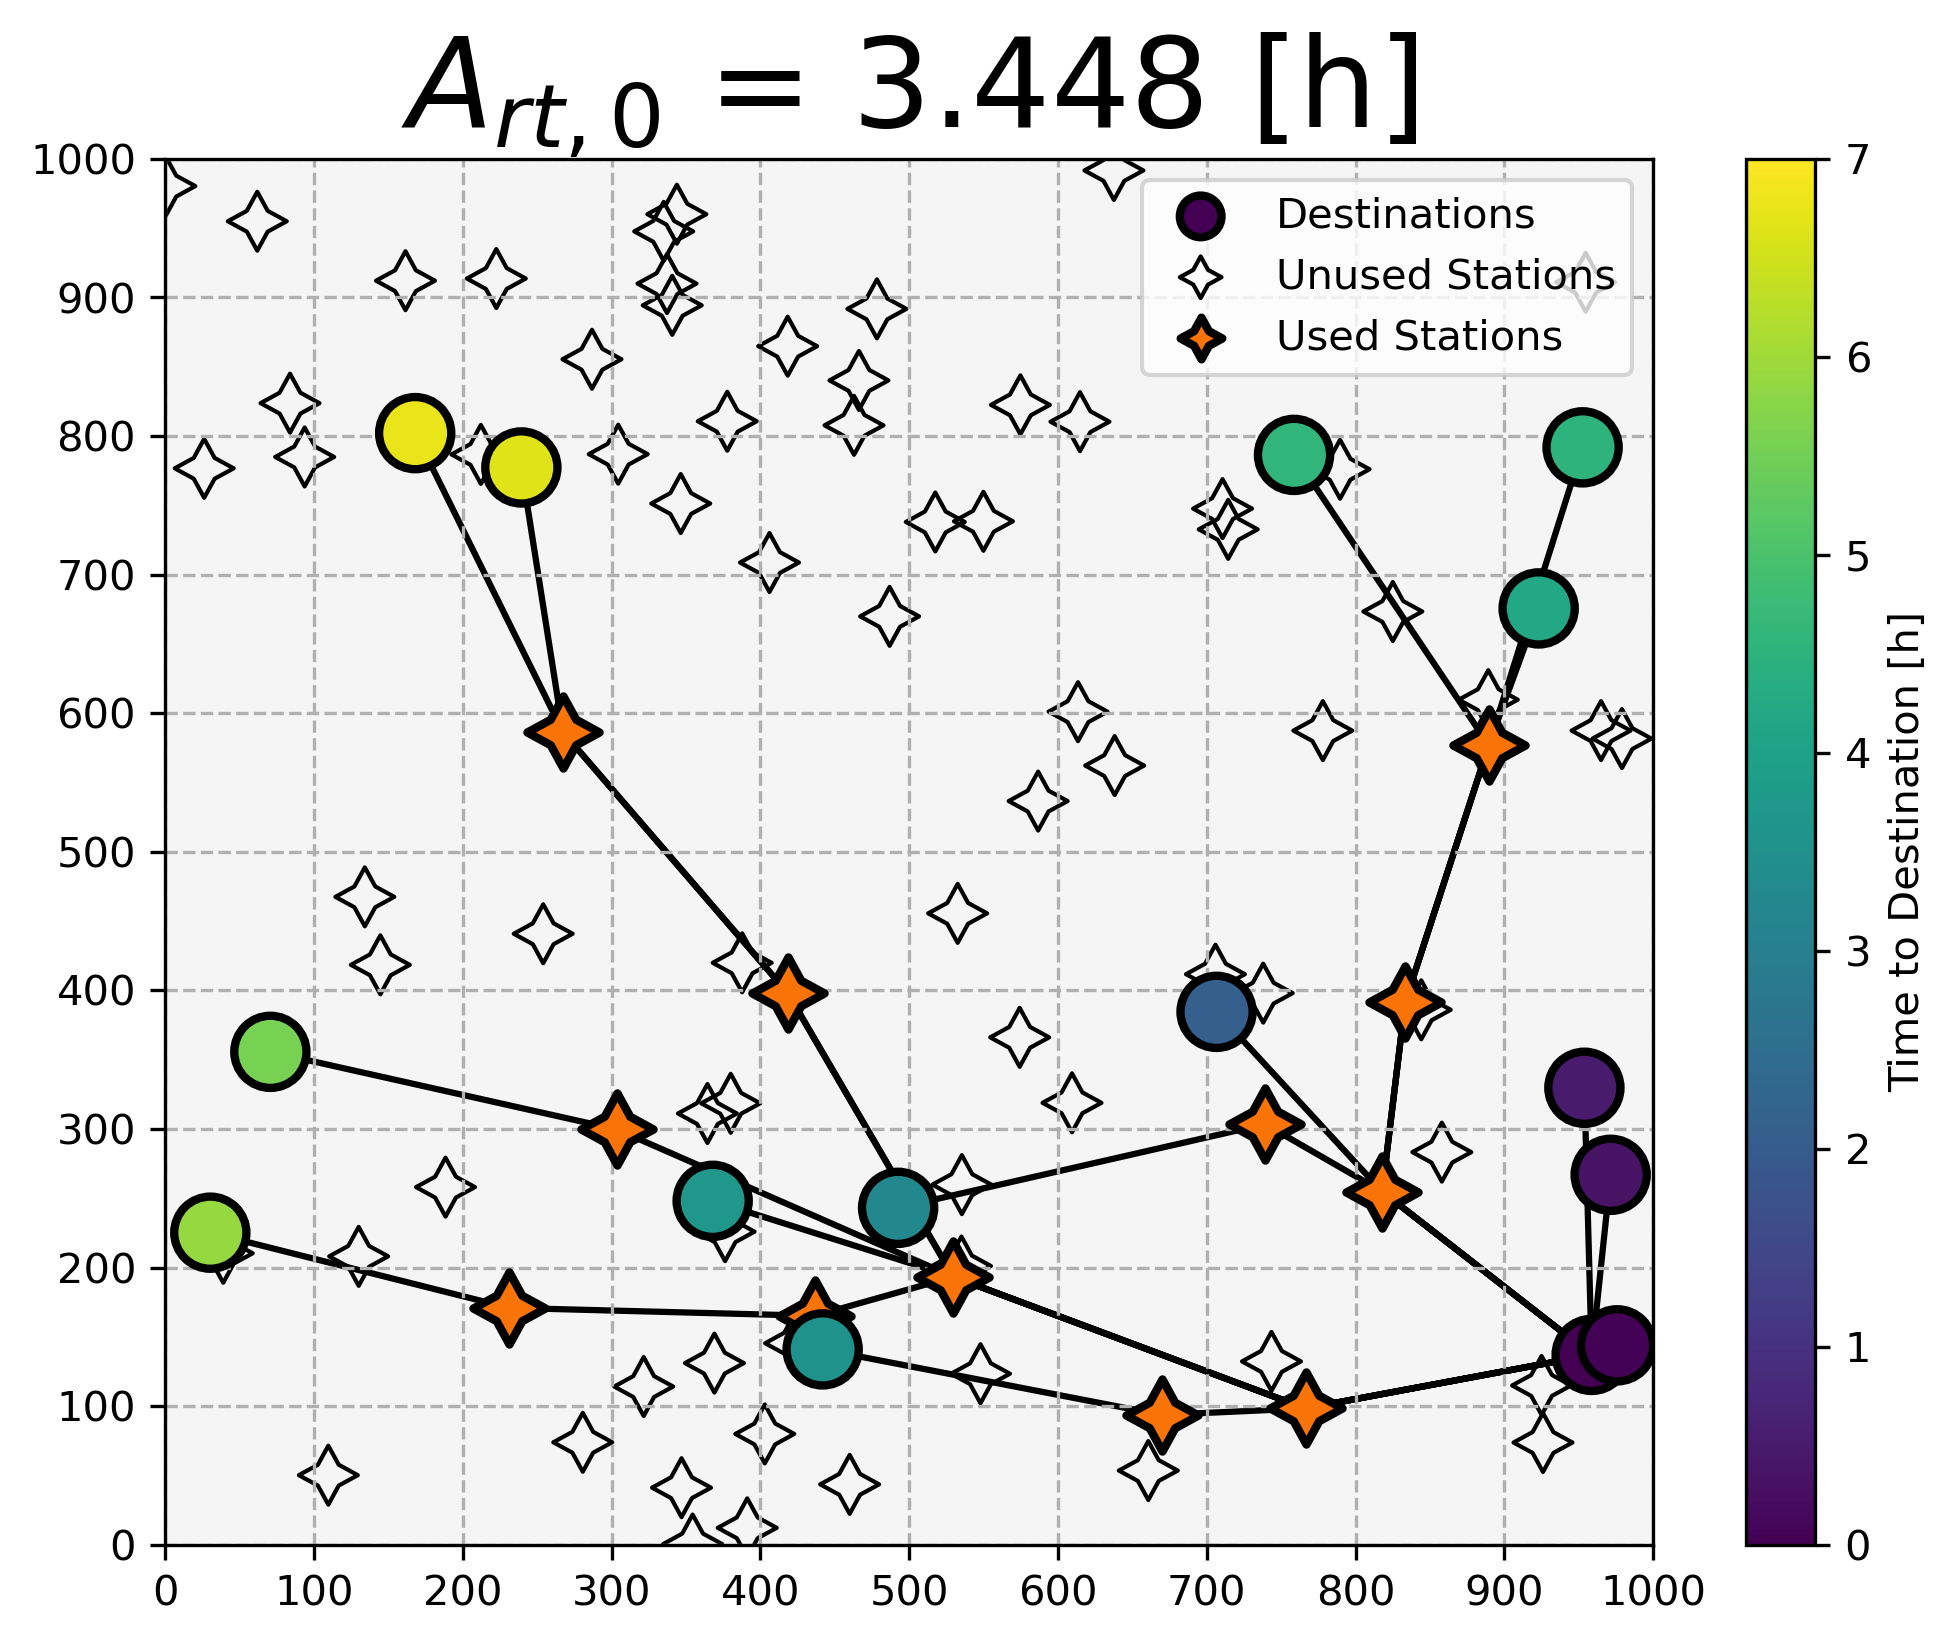
\includegraphics[width = \linewidth]{figs/random_example_high_reliability_cautious.png}
		\caption{High reliability, cautious}
	\end{subfigure}
	\begin{subfigure}[t]{.5\linewidth}
		\centering\captionsetup{width = .8\linewidth}
		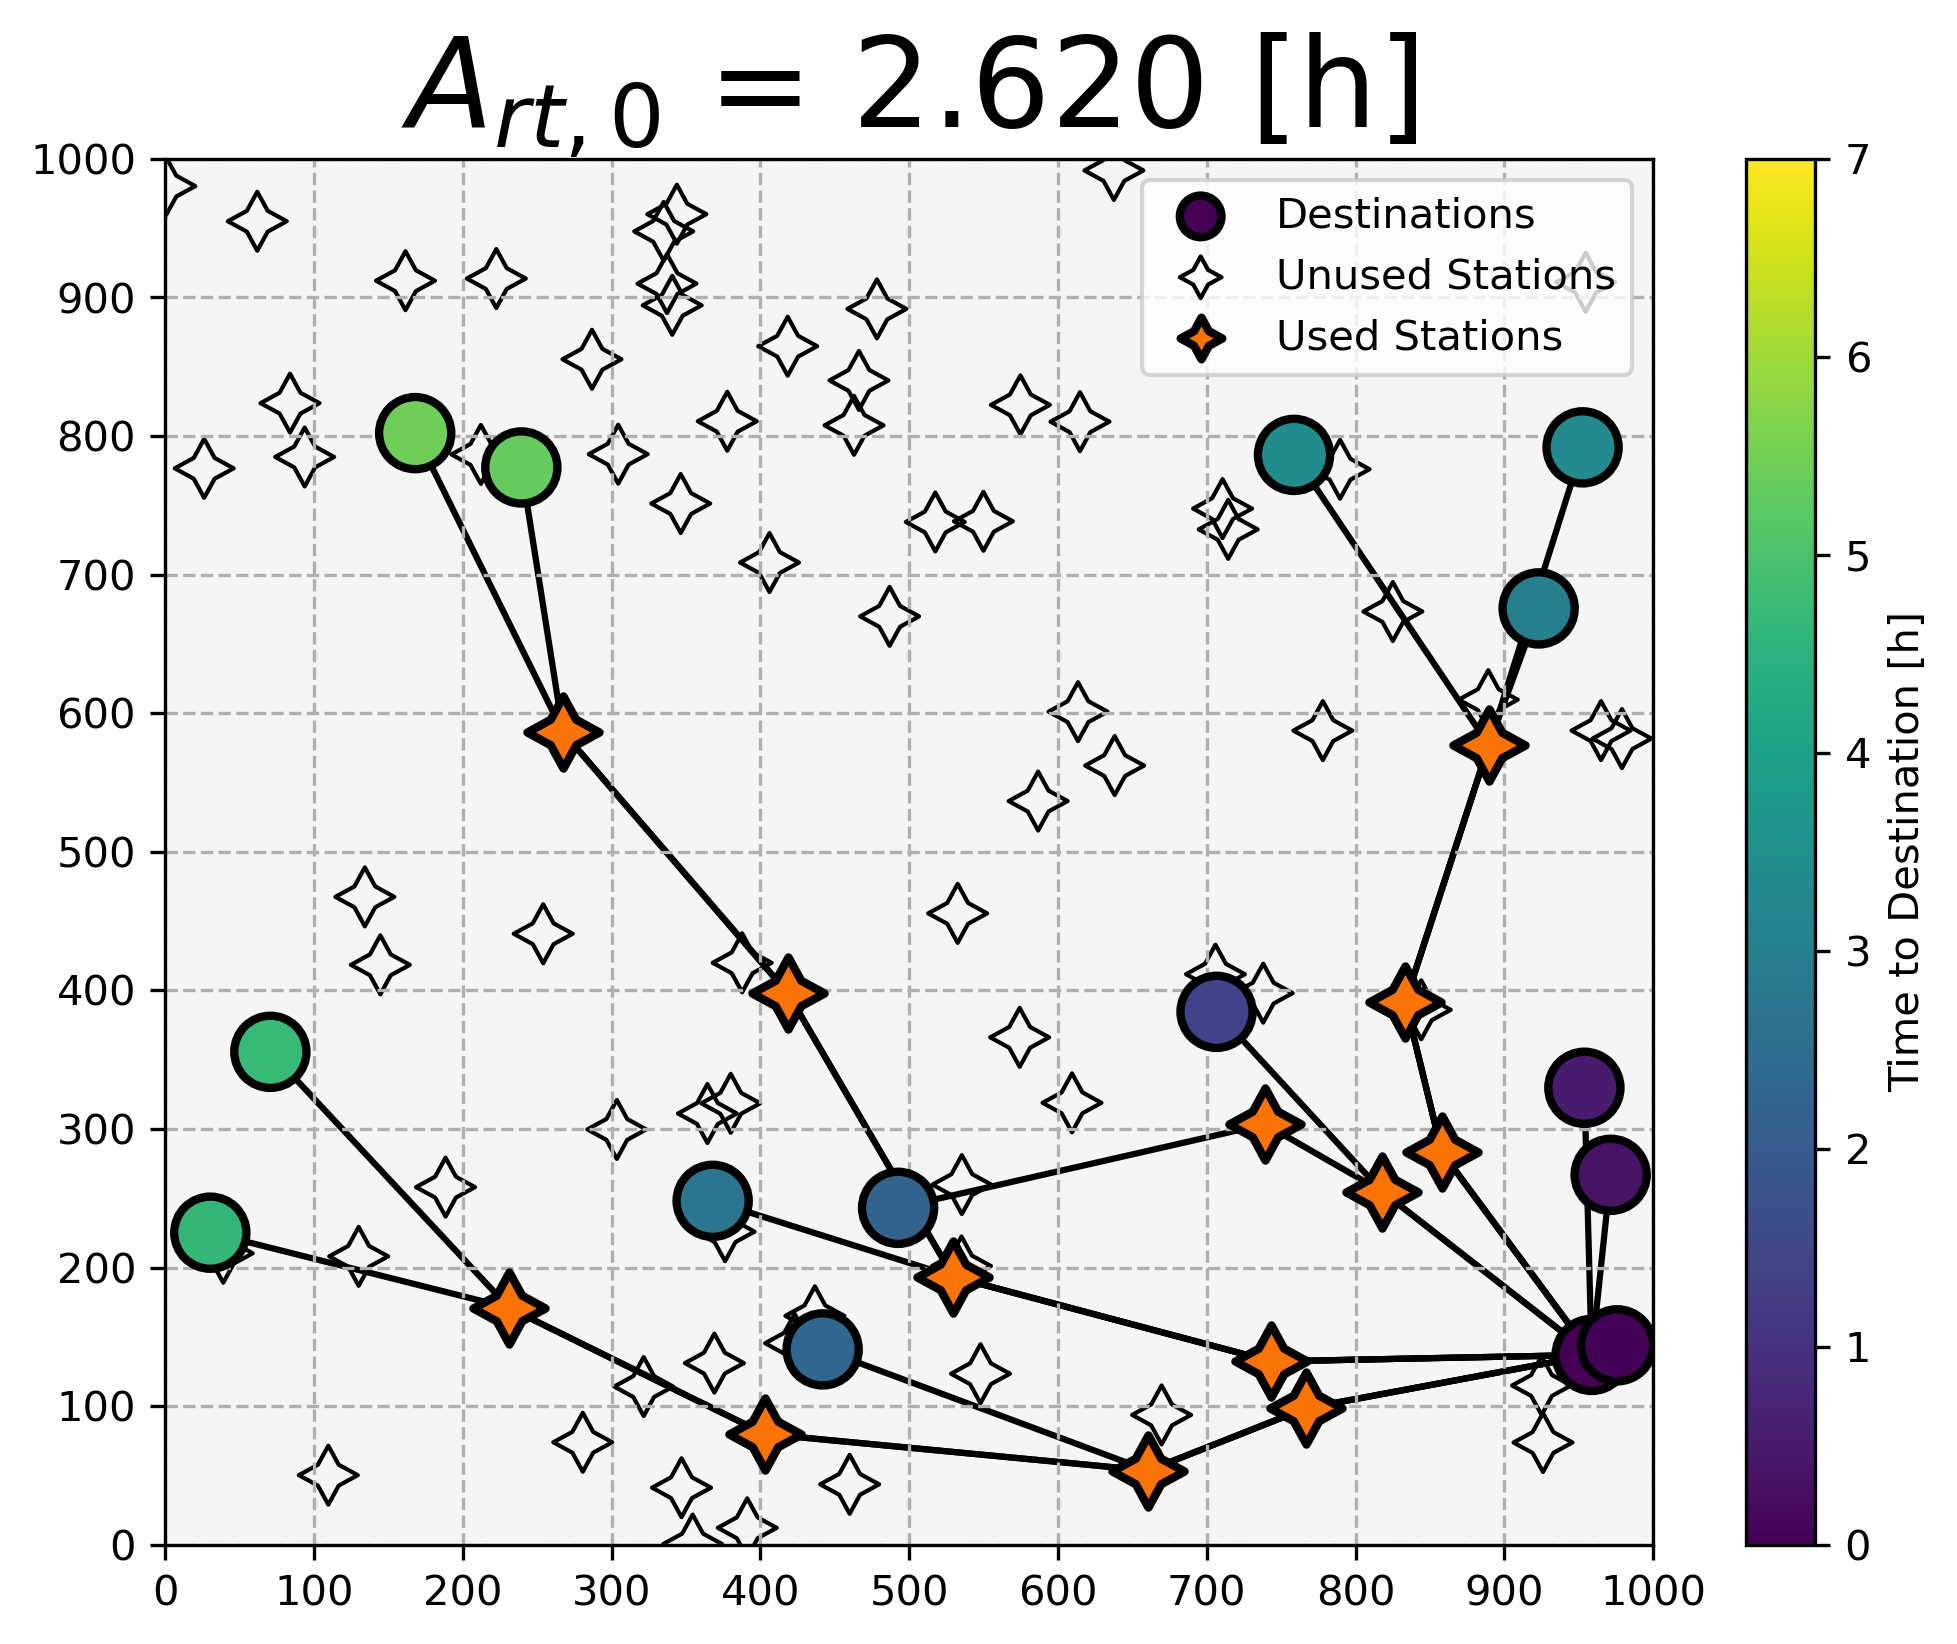
\includegraphics[width = \linewidth]{figs/random_example_low_reliability_aggressive.png}
		\caption{Low reliability, aggressive}
	\end{subfigure}%
	\begin{subfigure}[t]{.5\linewidth}
		\centering\captionsetup{width = .8\linewidth}
		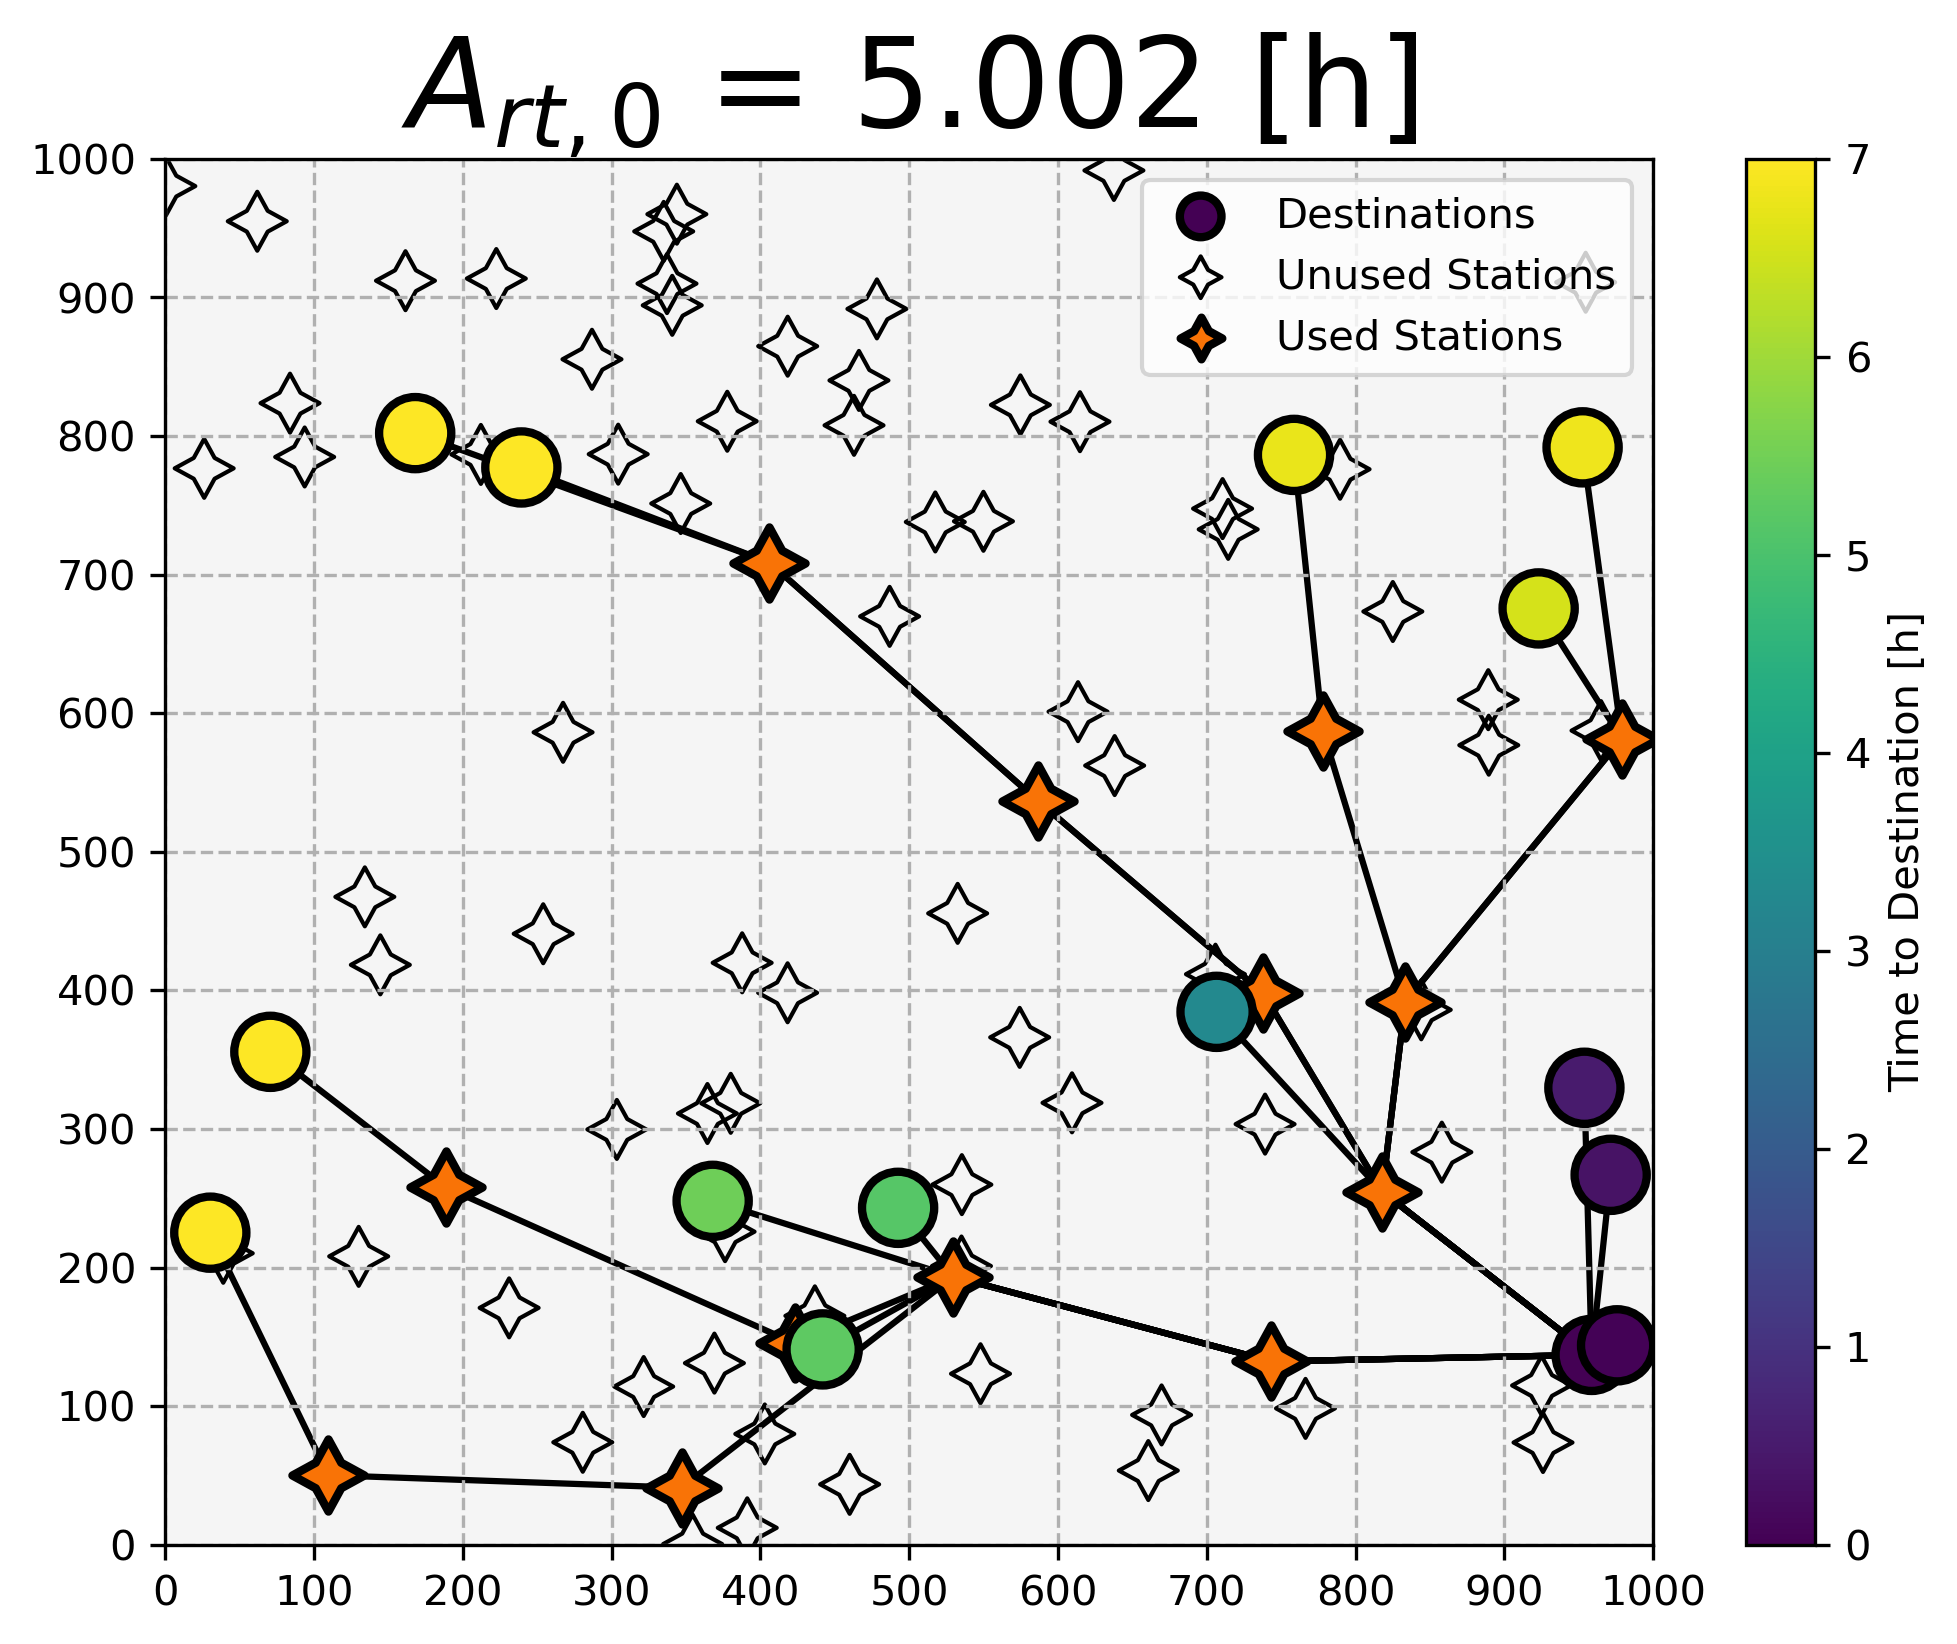
\includegraphics[width = \linewidth]{figs/random_example_low_reliability_cautious.png}
		\caption{Low reliability, cautious}
	\end{subfigure}
	\caption{Driver's perception of Specific Road-trip Accessibility for different drivers with different levels of charger reliability.}
	\label{fig:perceived_srta_random}
\end{figure}

The scenarios presented in Figure \ref{fig:perceived_srta_random} consider different levels of equipment reliability (75\% and 95\%) and different driver risk-attitudes (aggressive - $p_0 = 0,\ p_1 = .1$ and cautious - $p_0 = .9,\ p_1 = 1$). Specifically, the results consider Specific Road-Trip Accessibility as perceived by the driver. The aggressive driver is only concerned with the best 10\% of outcomes where the cautious driver is only concerned with the worst 10\% of outcomes. The differences in perceived costs-to-travel are quite stark between the aggressive and cautious driver in both cases but this difference is larger when reliability is low. In other words, the effects are additive from a perceived cost perspective. A manifestation of this gap is the different routes taken in the different scenarios. Perception is biased and not necessarily the best basis to evaluate costs-to-travel. The neutral expectations ($p_0 = 0,\ p_1 = 1$) of the routes taken by the drivers are shown in Figure \ref{fig:perceived_srta_random_n}.

\begin{figure}[H]
	\centering
	\begin{subfigure}[t]{.5\linewidth}
		\centering\captionsetup{width = .8\linewidth}
		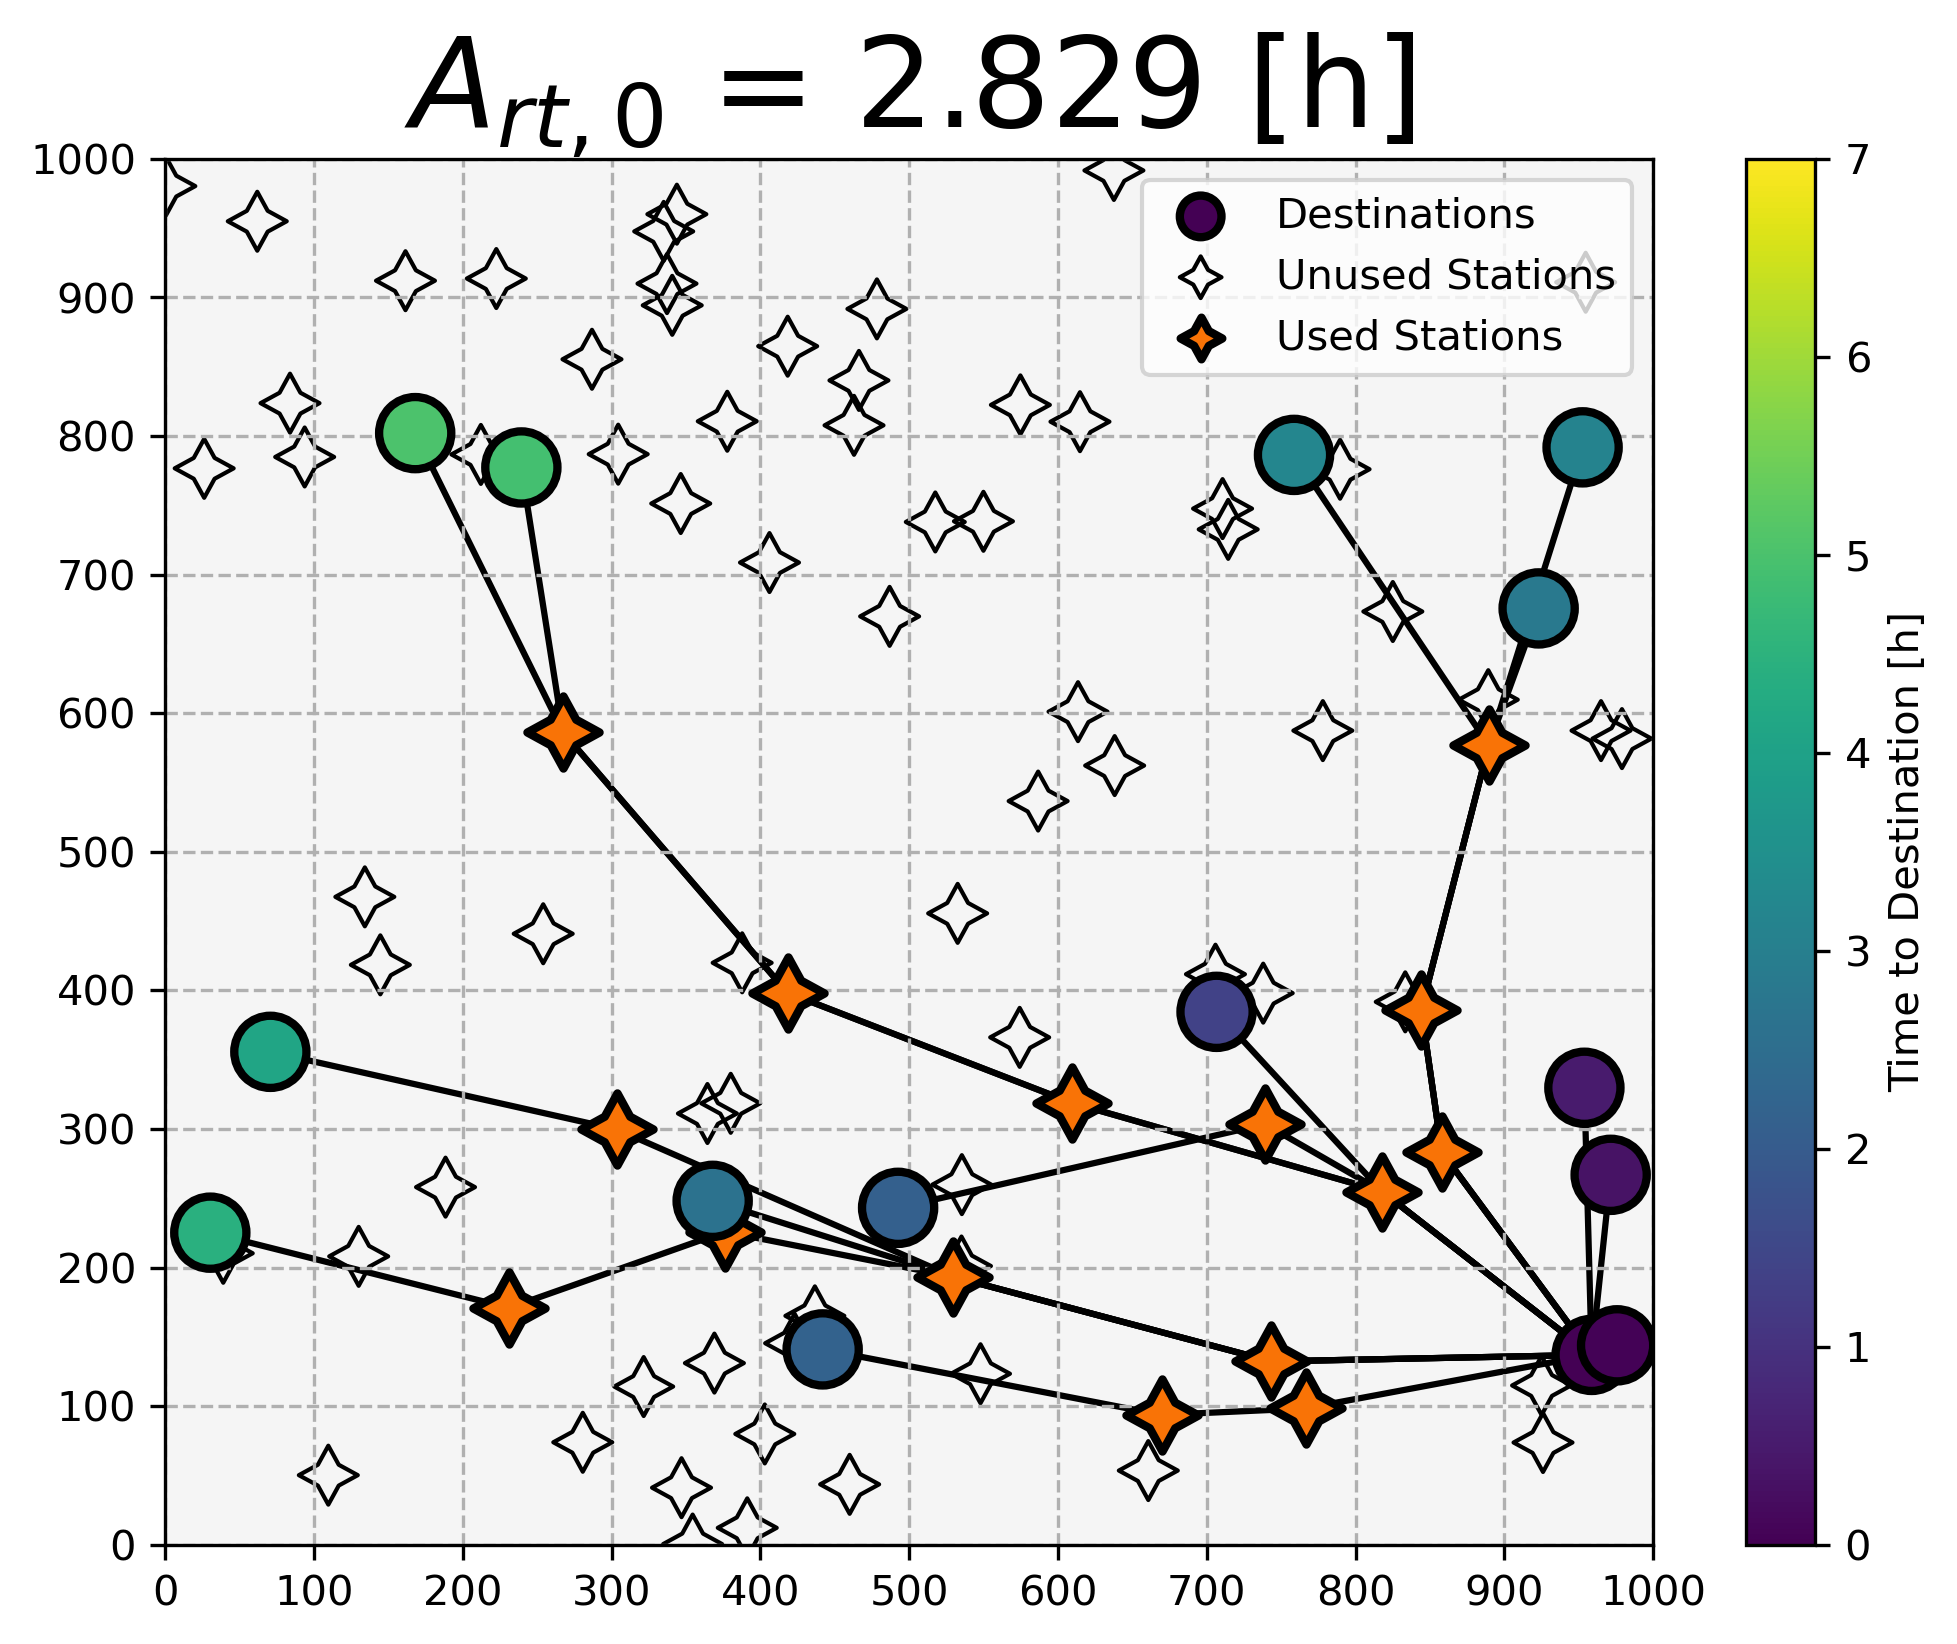
\includegraphics[width = \linewidth]{figs/random_example_high_reliability_aggressive_n.png}
		\caption{High reliability, aggressive}
	\end{subfigure}%
	\begin{subfigure}[t]{.5\linewidth}
		\centering\captionsetup{width = .8\linewidth}
		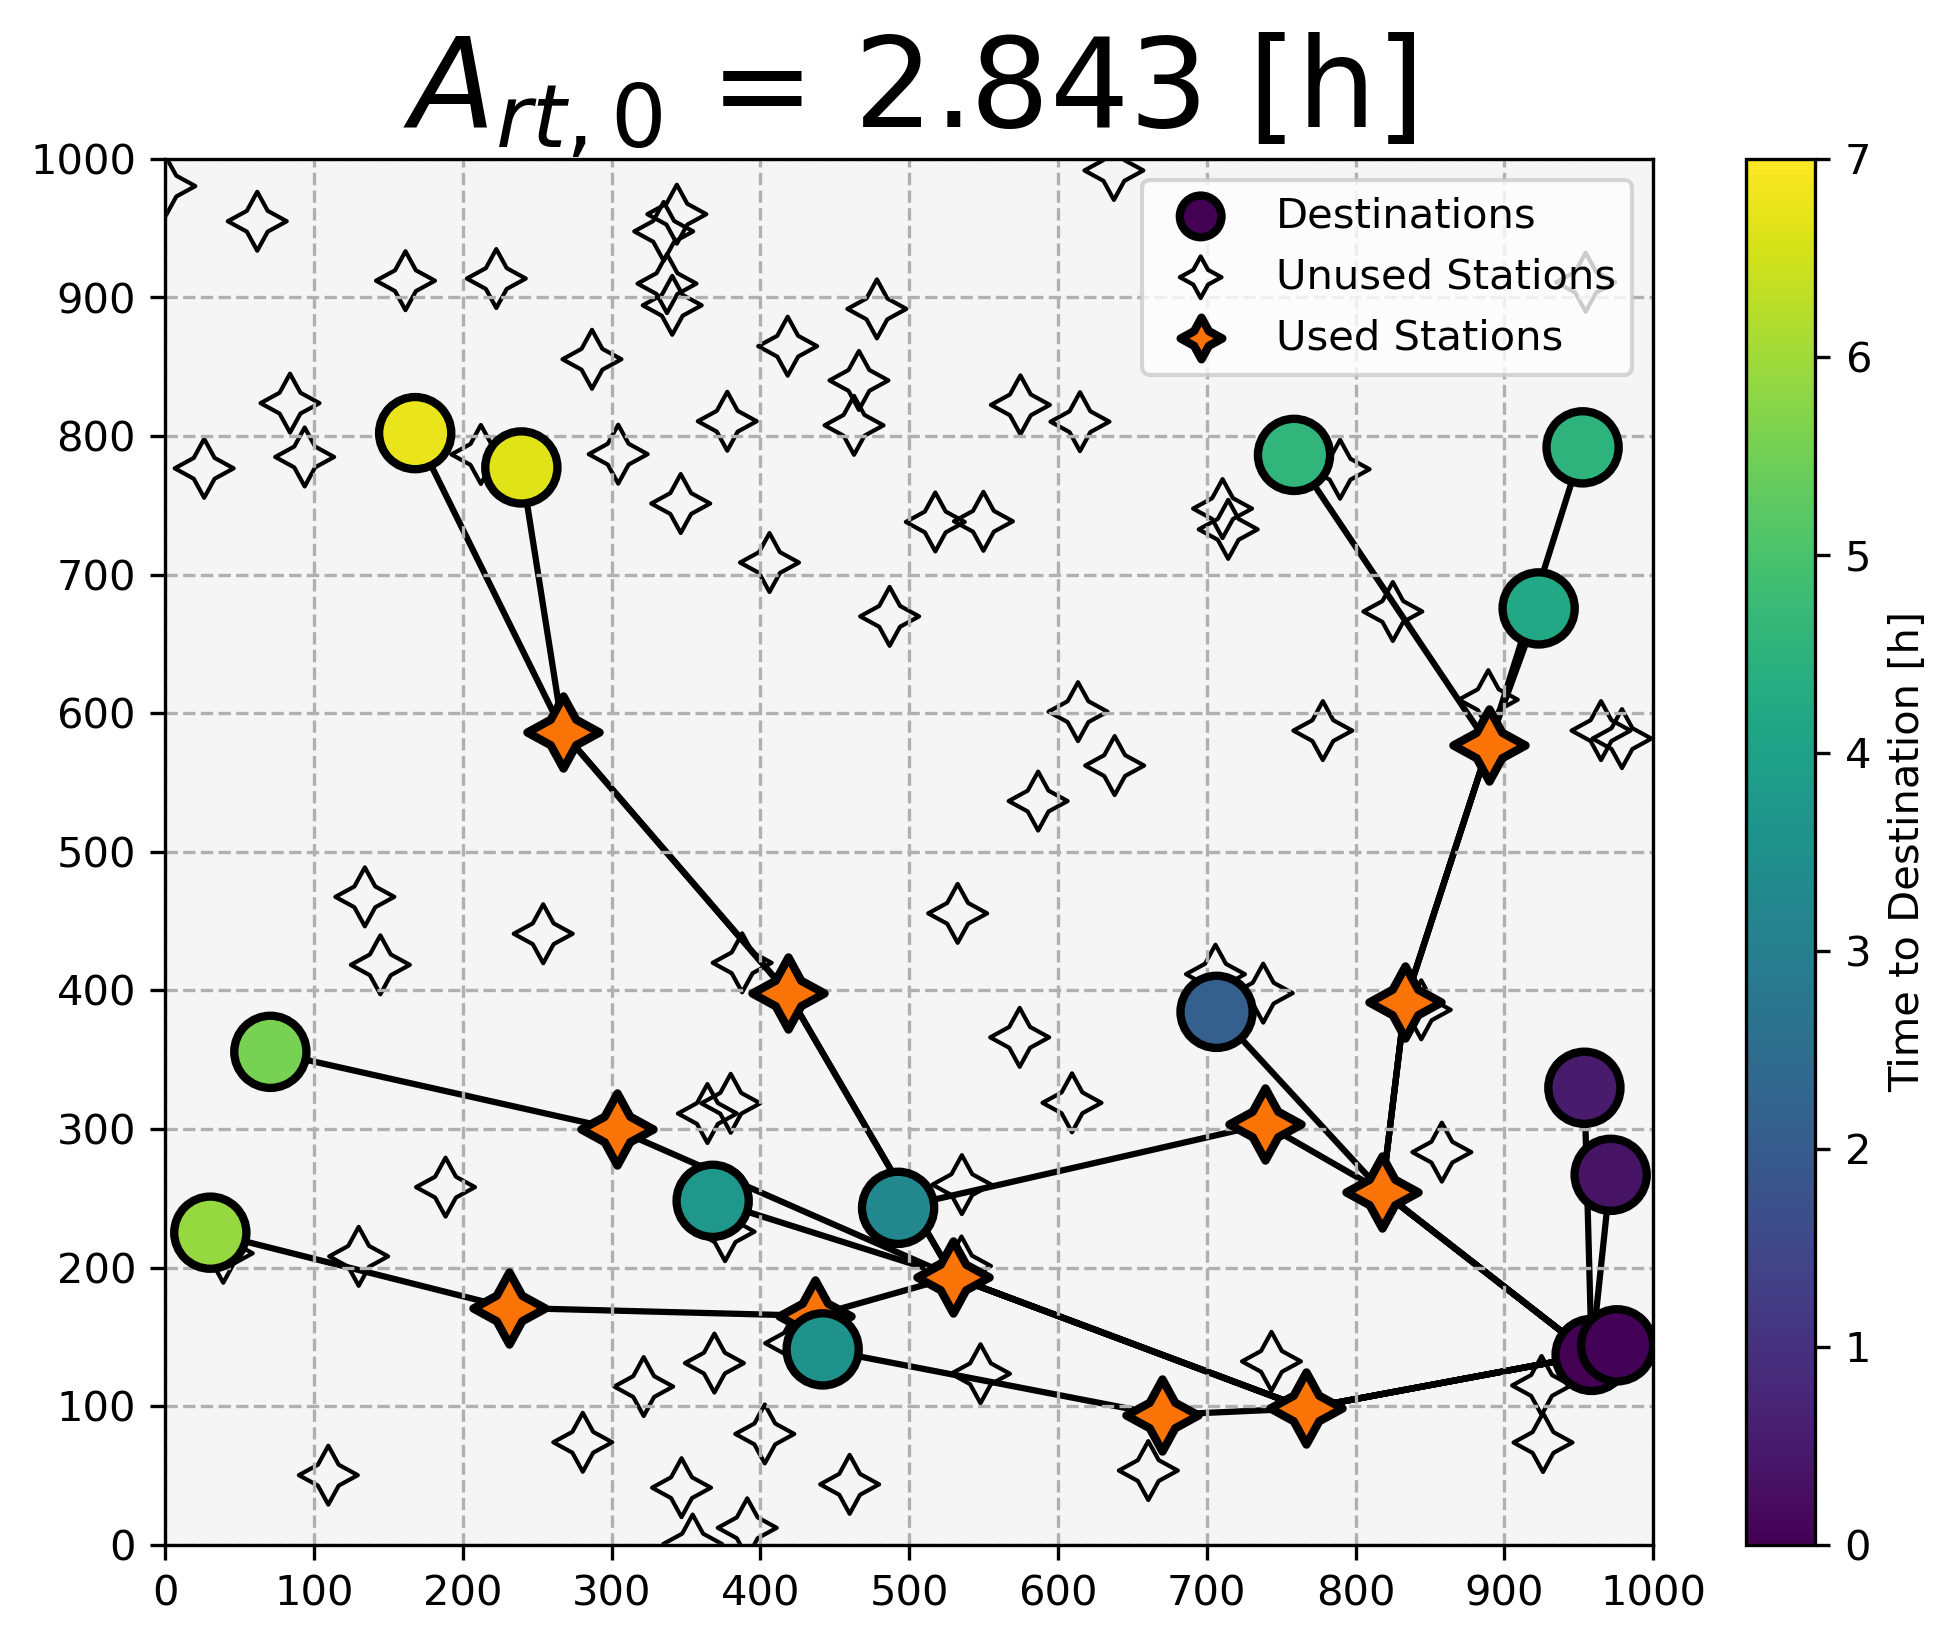
\includegraphics[width = \linewidth]{figs/random_example_high_reliability_cautious_n.png}
		\caption{High reliability, cautious}
	\end{subfigure}
	\begin{subfigure}[t]{.5\linewidth}
		\centering\captionsetup{width = .8\linewidth}
		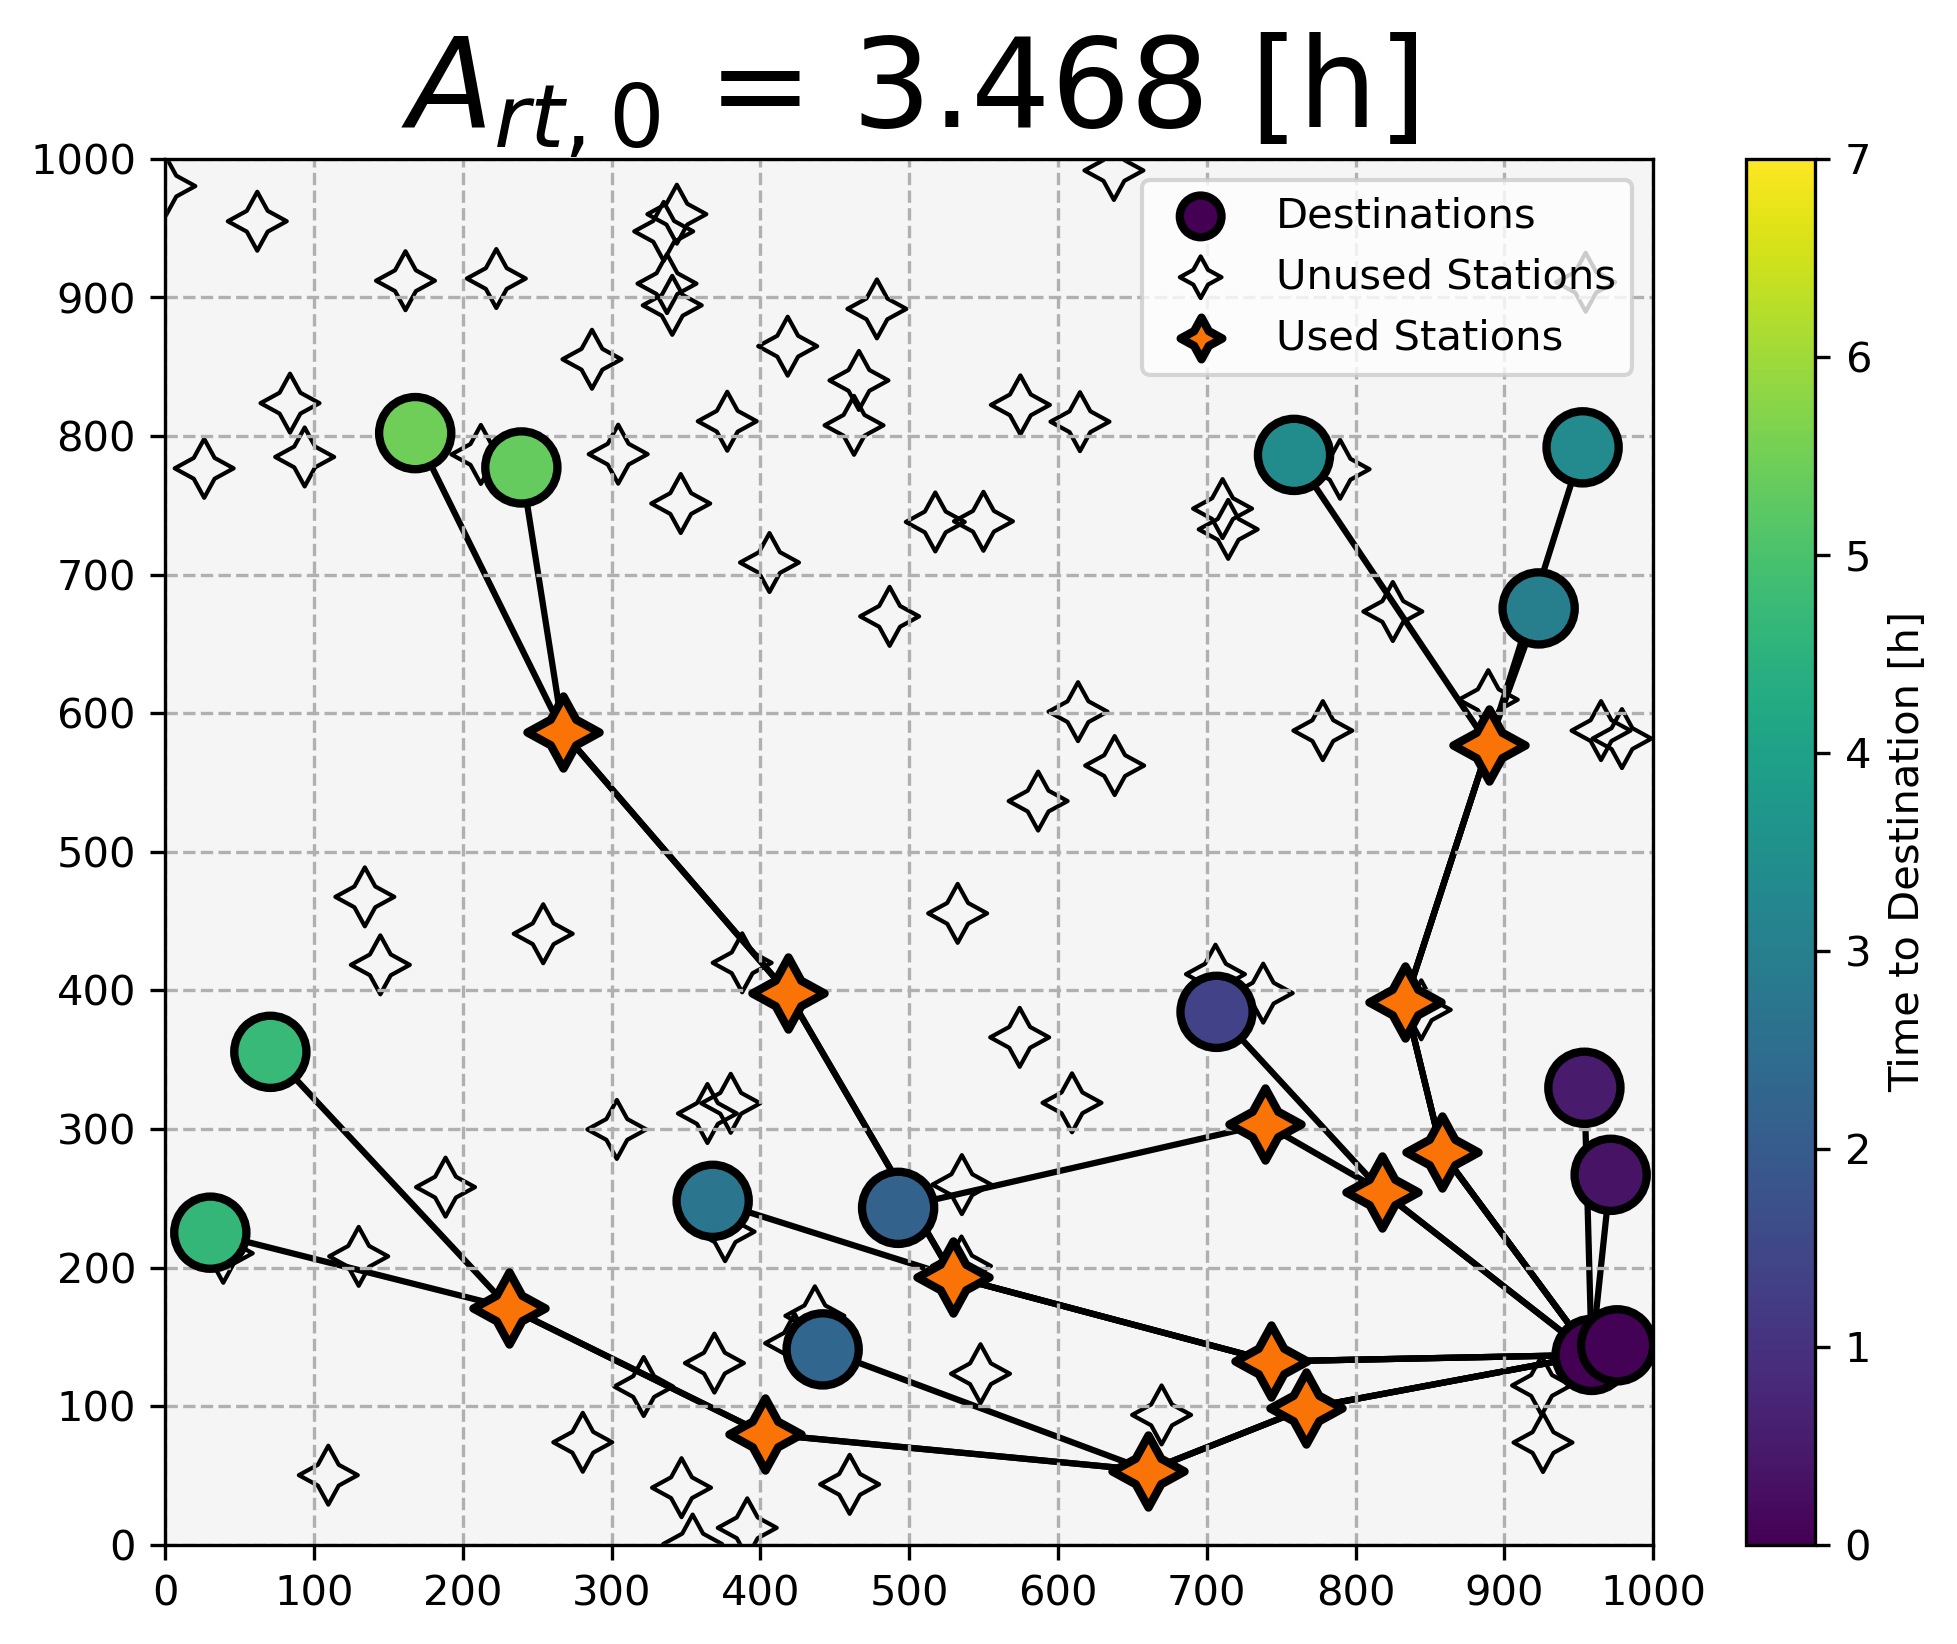
\includegraphics[width = \linewidth]{figs/random_example_low_reliability_aggressive_n.png}
		\caption{Low reliability, aggressive}
	\end{subfigure}%
	\begin{subfigure}[t]{.5\linewidth}
		\centering\captionsetup{width = .8\linewidth}
		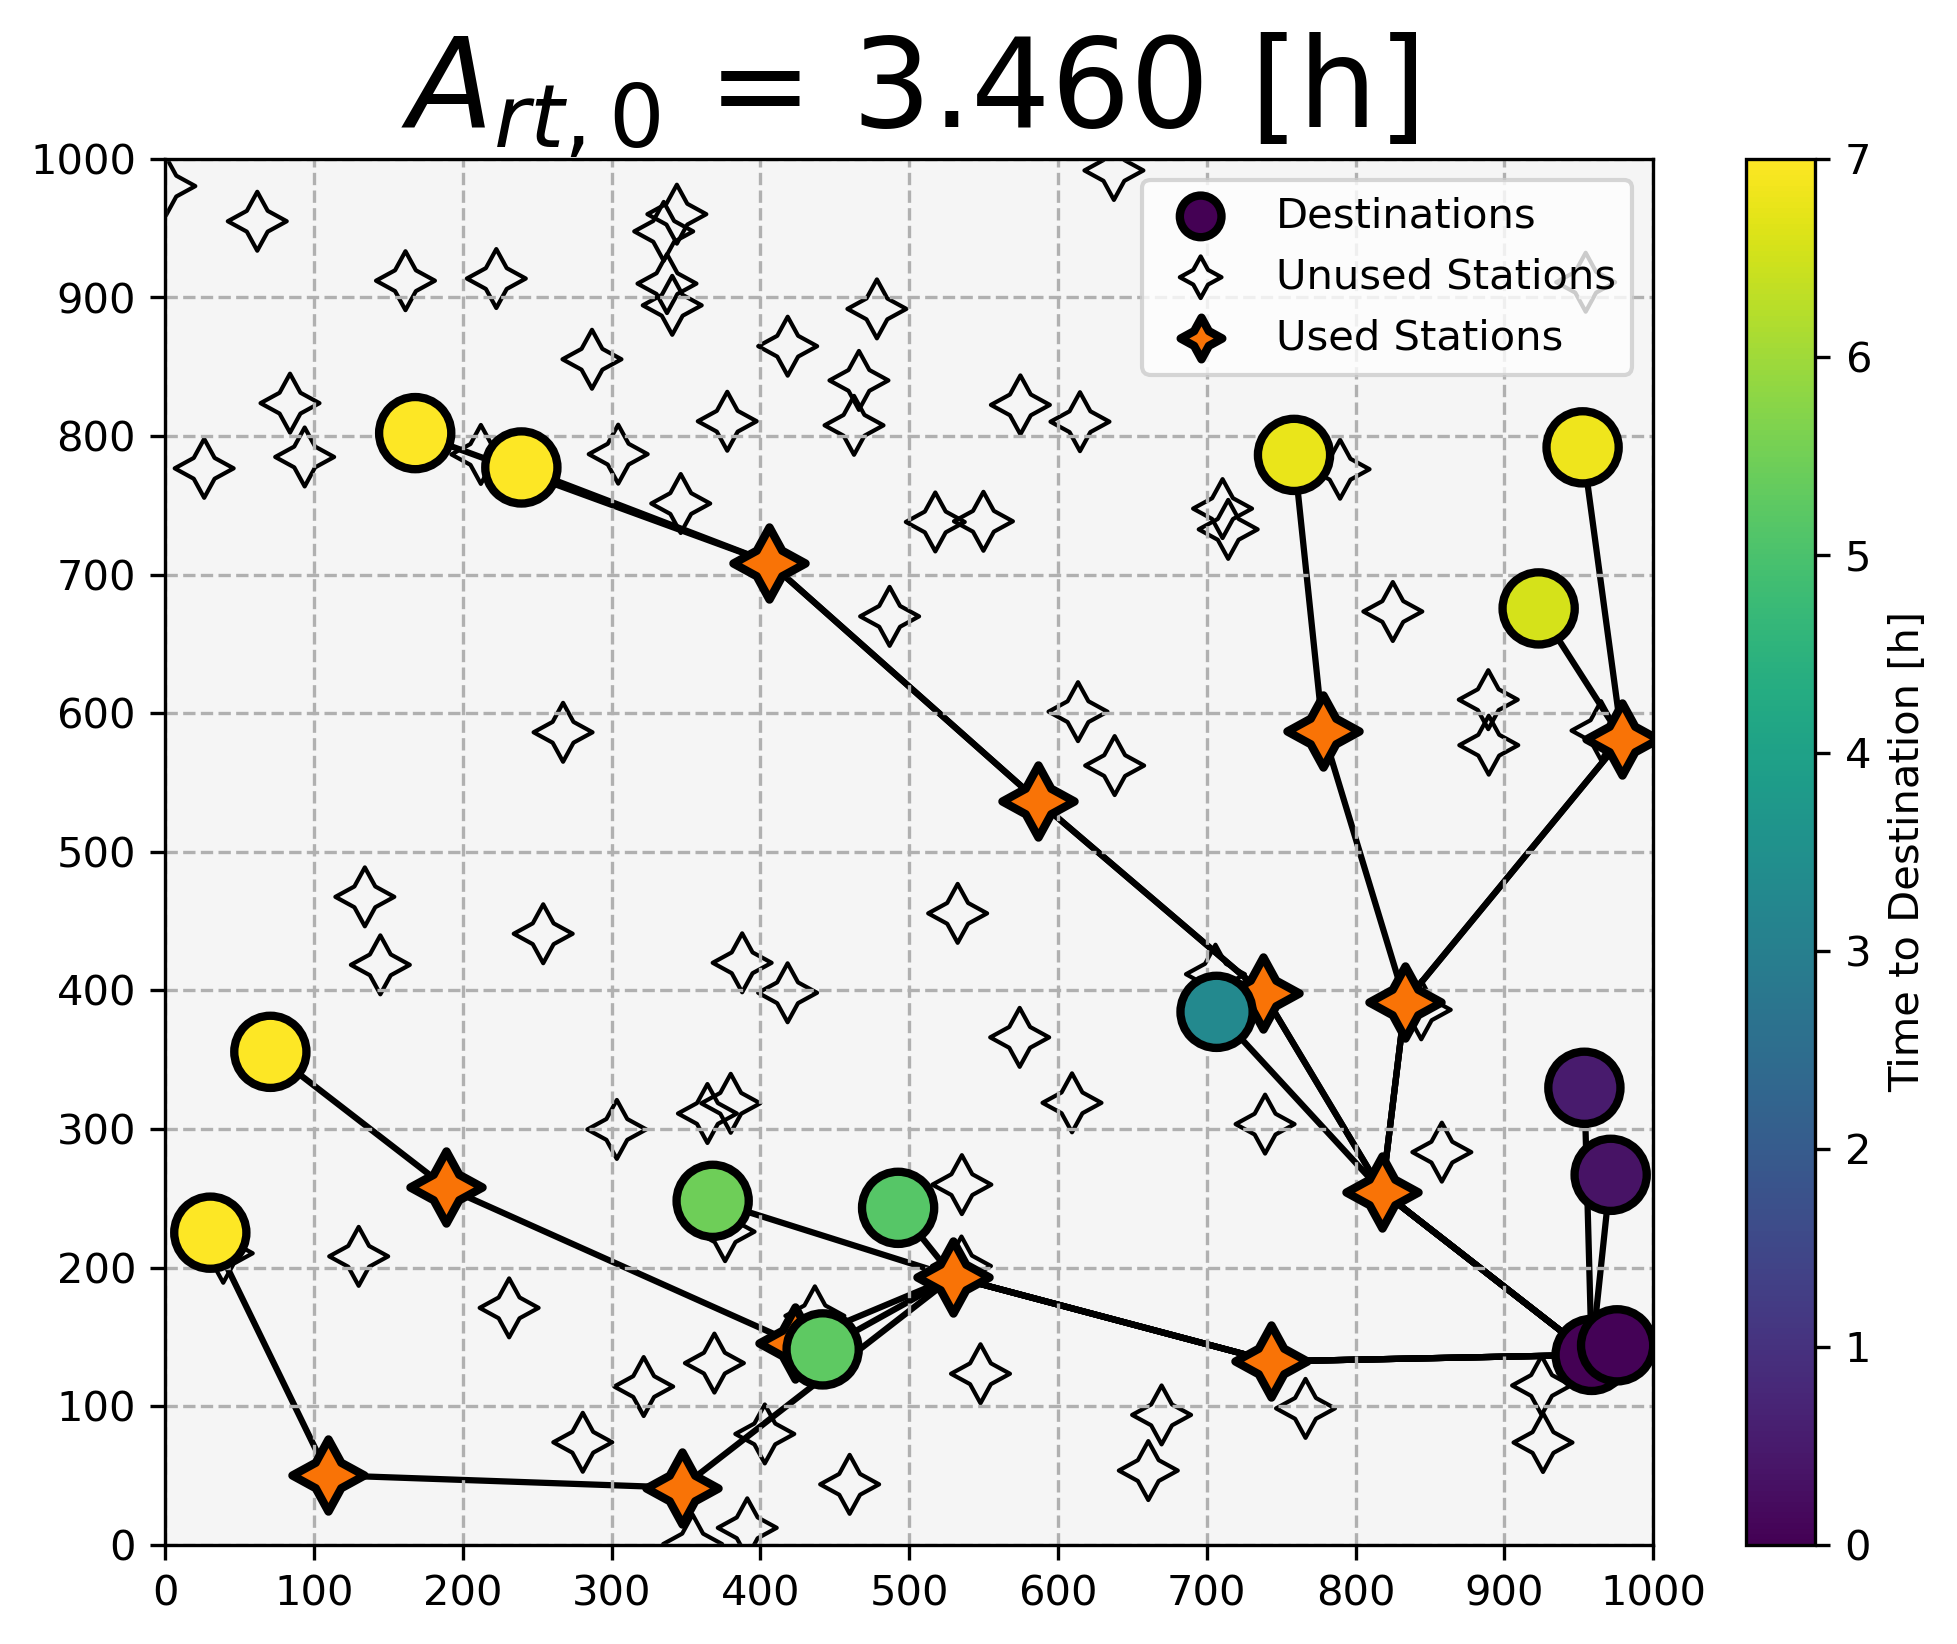
\includegraphics[width = \linewidth]{figs/random_example_low_reliability_cautious_n.png}
		\caption{Low reliability, cautious}
	\end{subfigure}
	\caption{Neutral expectation of Specific Road-trip Accessibility for different drivers with different levels of charger reliability.}
	\label{fig:perceived_srta_random_n}
\end{figure}

The neutral expectations tell a different story. For the different levels of reliability, neutral expectations of costs-to-travel are similar for the routes selected by the aggressive and cautious drivers. The differences between biased and neutral perception are easy to understand. Both drivers selected routes based on a subset of the information and these routes are non-optimal when all information is considered. Drivers may adjust their priors over time but policy can only control the fundamentals. Thus, it is recommended to consider bias in route planning but neutral expectation in evaluation.

The composition of the routes taken by the drivers in the randomly generated example demonstrate an interesting dynamic as seen in Table \ref{tab:distances_redundancy}.

\begin{table}[H]
	\centering
	\caption{Average route distances and chargers per station utilized for example scenarios}
	\label{tab:distances_redundancy}
	\begin{tabular}{|C{.25\linewidth}|C{.25\linewidth}|C{.25\linewidth}|C{.25\linewidth}|}
		\hline Reliability & Risk-Attitude & Average Route Distance [km] & Chargers per Station Utilized [-] \\
		\hline High & Aggressive & 558.827 & 3.871 \\
		\hline High & Cautious & 578.505 & 4.290 \\
		\hline Low & Aggressive & 575.947 & 4.063 \\
		\hline Low & Cautious & 574.953 & 3.750 \\
		\hline
	\end{tabular}
\end{table}

When reliability is high, the aggressive driver opts for a more direct path where the cautious driver favors a path with higher charger redundancy in-station. However, when reliability is low the reverse happens. This is because, in the low reliability scenario, completely failed stations come into play and the cautious driver tends to stick to areas with higher redundancy between-station even if this means accepting perceived longer queues. The aggressive driver, ignoring the worst case scenario of being stranded, opts for the lower expected queuing time to be found in high redundancy stations.

\section*{California Case Study}

The randomly generated example is informative but does not reflect any actual \gls{sng}. In order to see effects on a more representative basis a case study is performed on the state of California using information on the states DC EV \gls{sng} with modes of common \glspl{bev} which enjoy different levels of access.

\subsection*{Background}

The state of California is geographically large and contains major population centers distributed across the state. Major road transportation corridors form connections between the state's population centers and with population centers in adjacent states. This case study concerns the long-trip accessibility of California's road transportation network. For the purposes of analysis, 15 important cities in California and adjacent states were selected. Non-California locations are represented by the most-likely departure locations at the California state line. Because the state-line locations are midpoints the required arrival \gls{soc} at these points is set at 50\% where it is set at 20\% for all others. These locations are enumerated in Table \ref{tab:locations}.

\begin{table}[H]
	\centering
	\caption{Locations Considered for Long Trip Accessibility}
	\label{tab:locations}
	\begin{tabular}{|C{\linewidth * 1 / 3}|C{\linewidth * 2 / 3}|}
		\hline Index & Location \\
		\hline 0 & Crescent City \\
		\hline 1 & Yreka \\
		\hline 2 & Redding \\
		\hline 3 & Chico \\
		\hline 4 & Reno (State Line) \\
		\hline 5 & Sacramento \\
		\hline 6 & Stockton \\
		\hline 7 & San Francisco \\
		\hline 8 & San Jose \\
		\hline 9 & Fresno \\
		\hline 10 & Las Vegas (State Line) \\
		\hline 11 & Bakersfield \\
		\hline 12 & Los Angeles \\
		\hline 13 & Phoenix (State Line) \\
		\hline 14 & San Diego \\
		\hline
	\end{tabular}
\end{table}

For long trips, \glspl{bev} will rely on DC charging stations. The locations of all DC charging stations in California are available from AFDC \cite{afdc_2023}. In may 2024 \gls{afdc} listed 2,149 active stations with at least 1 DC charger. This number is somewhat misleading as certain networks report each charger as an individual station even if within line-of-sight of one-another. After merging all stations of the same network which are within 100 meters direct distance of each other the number of stations becomes 1,689. California's DC charging stations include proprietary (vehicle \gls{oem} owned and operated) stations such as Tesla Superchargers and the Rivian Adventure network as well as non-proprietary stations such as those operated by ChargePoint, Electrify America, eVgo, and others. The selected locations and DC charging stations are mapped in Figure \ref{fig:california_stations}.

\end{multicols}

\begin{figure}[H]
	\begin{subfigure}{.5\linewidth}
		\centering
		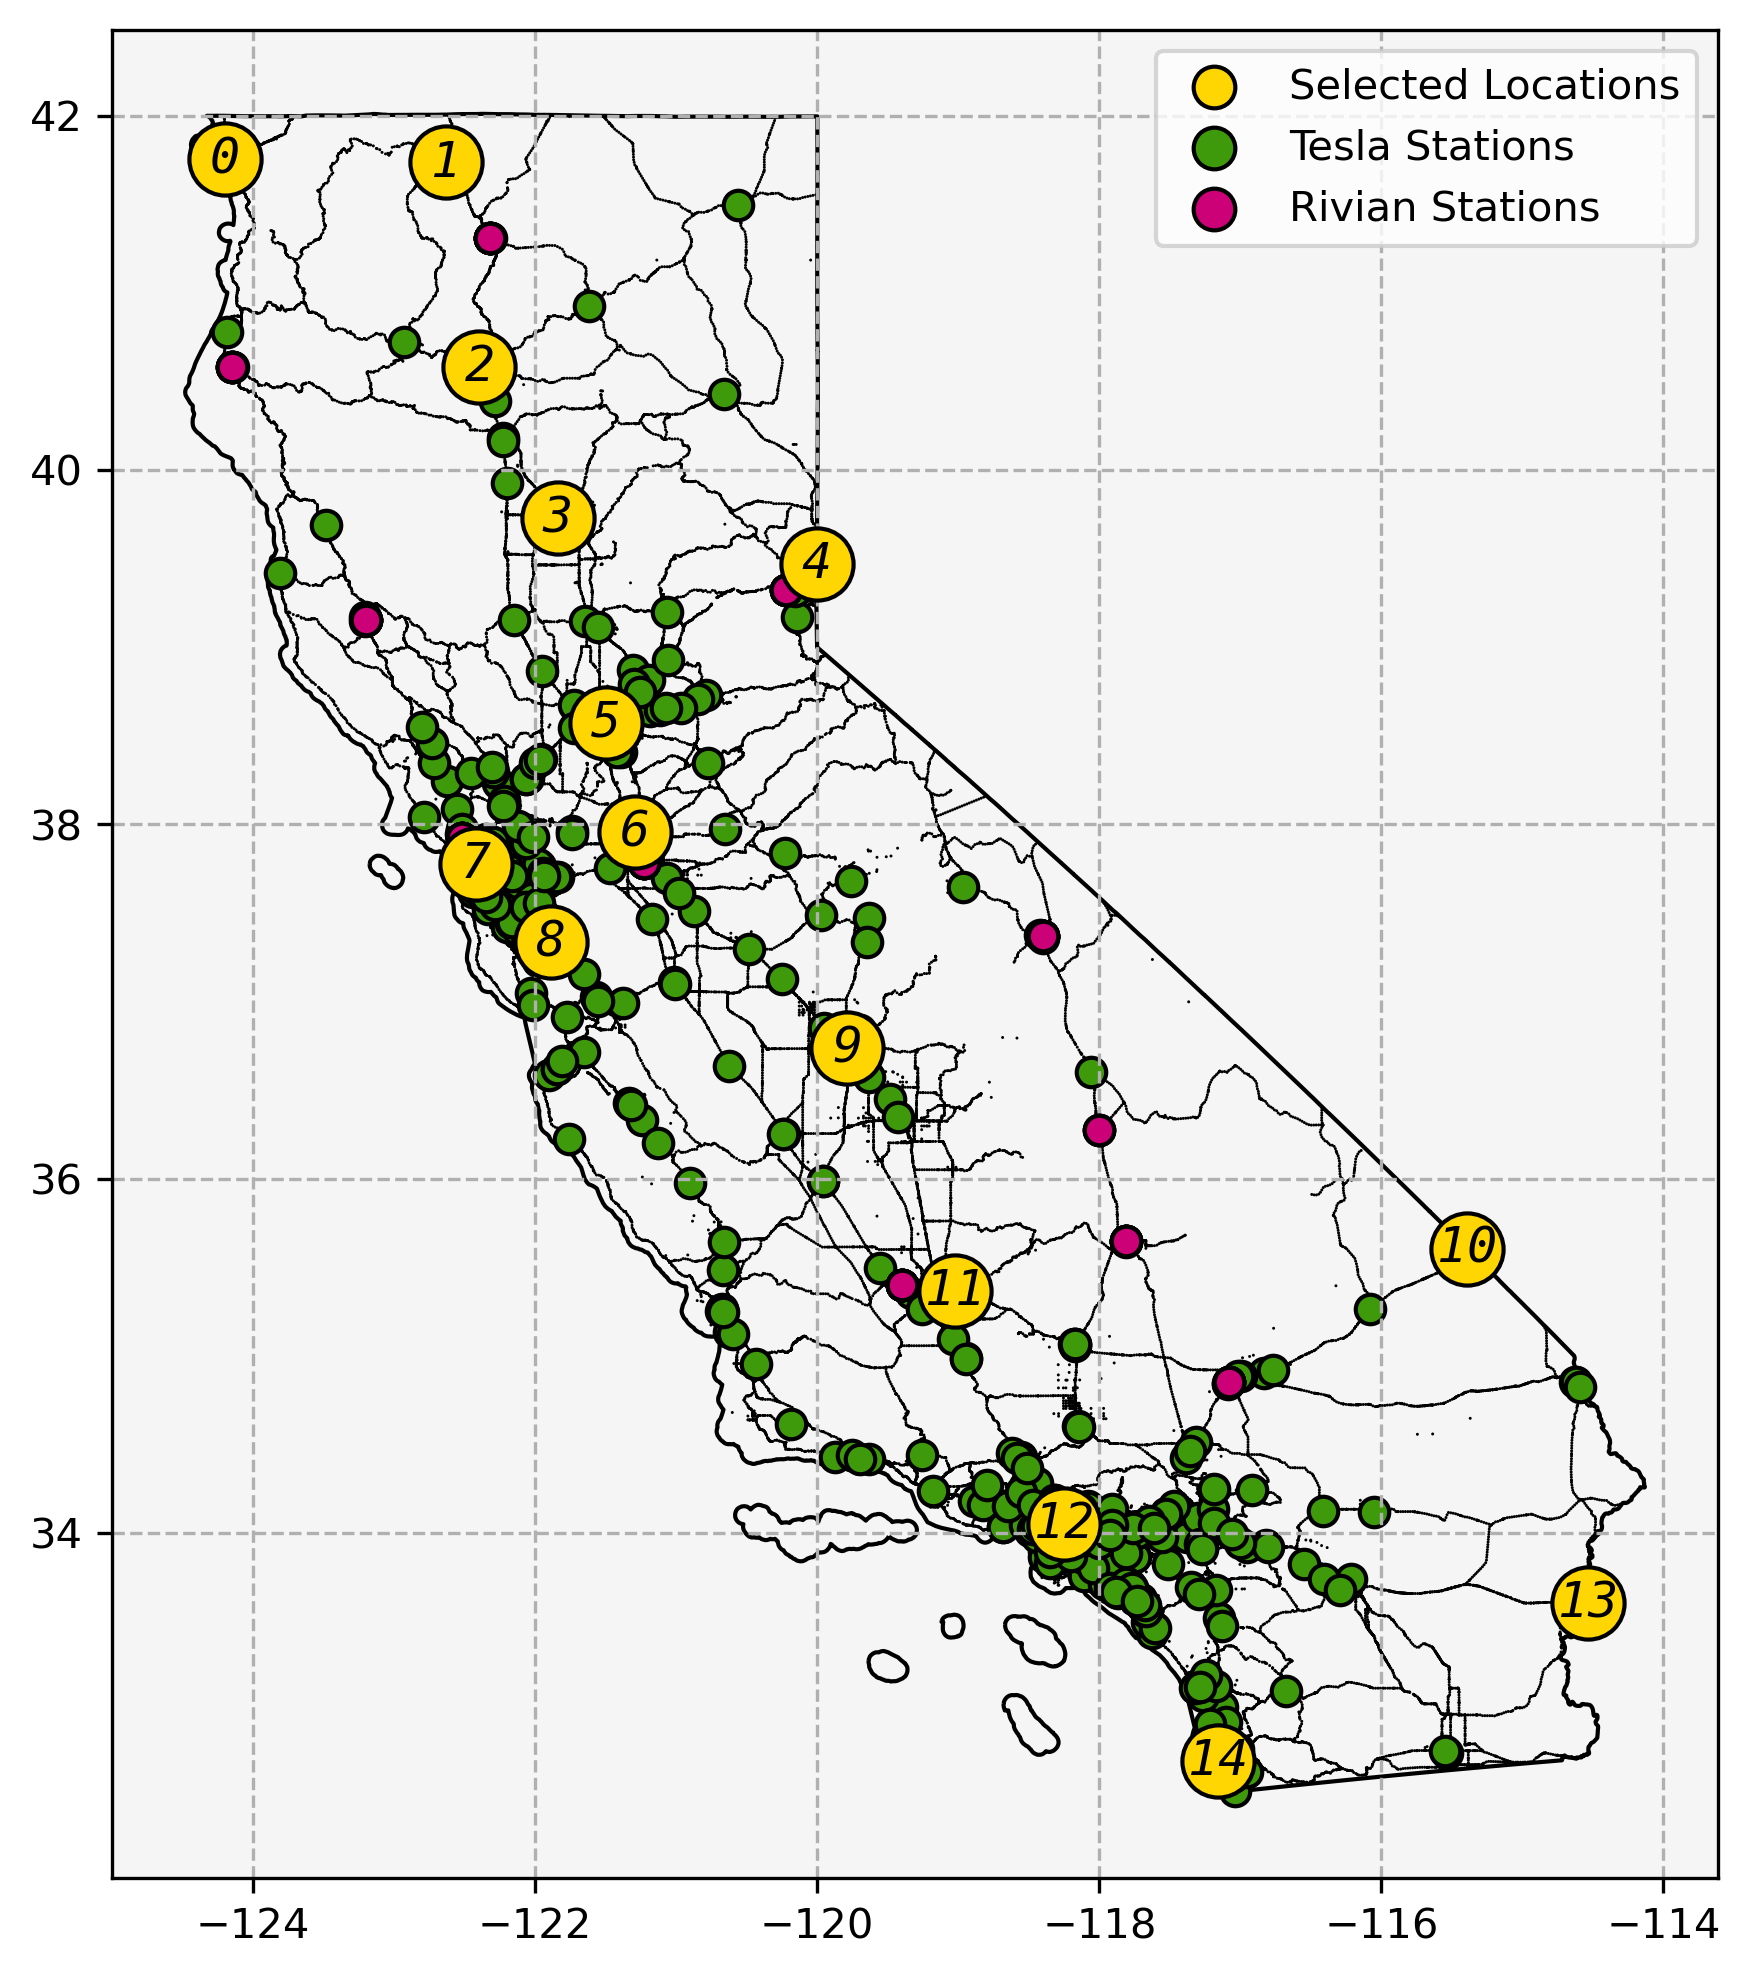
\includegraphics[width = \linewidth]{figs/California_SNG_P.png}
		\caption{Proprietary Stations}
	\end{subfigure}%
	\begin{subfigure}{.5\linewidth}
		\centering
		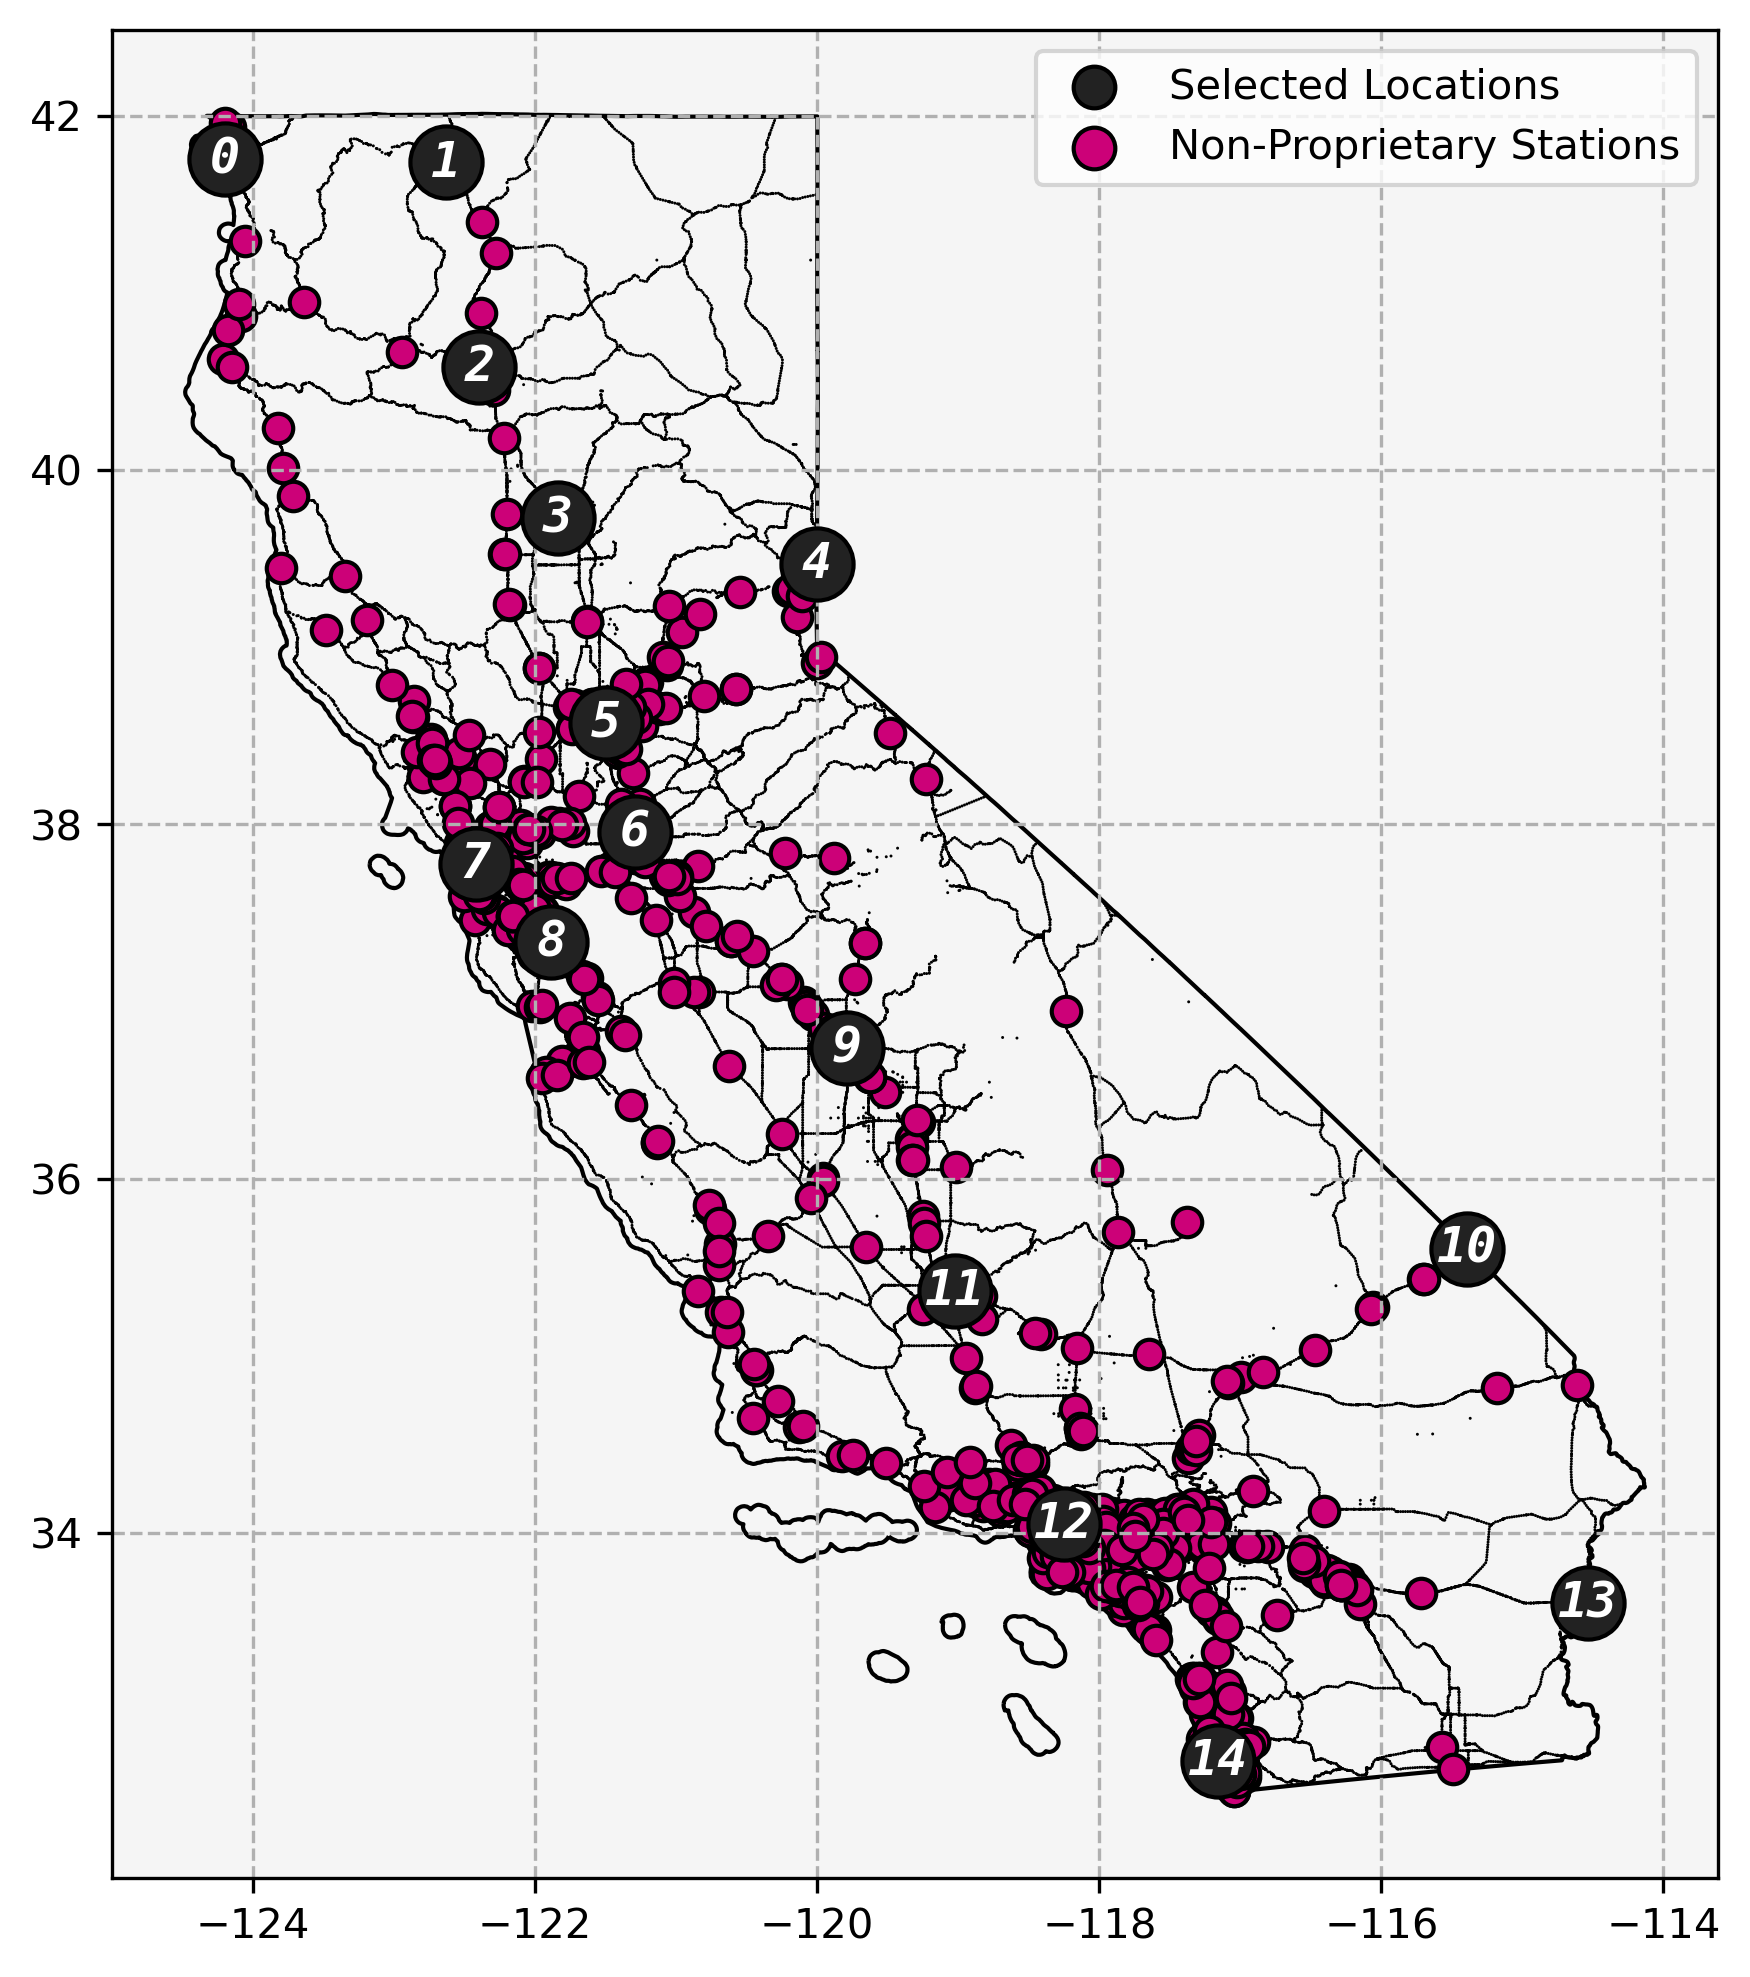
\includegraphics[width = \linewidth]{figs/California_SNG_NP.png}
		\caption{Non-Proprietary Stations}
	\end{subfigure}
	\caption{California DC charging stations from \gls{afdc} (May 2024)}
	\label{fig:california_stations}
\end{figure}

\begin{multicols}{2}

The proprietary and non-proprietary networks in California are neither equivalent nor isomorphic. There are 419 Tesla and 16 Rivian DC charging stations in the state as compared to 1,254 non-proprietary DC charging stations. In practice, many of these stations will be of little use for long distance travel being located far away from primary and secondary roads. Considering only those stations within 1 km of a highway as "corridor" chargers, there are a total of 477 corridor DC charging stations. Of the corridor stations, 143 are Tesla stations, 6 Rivian stations, and 328 non-Proprietary stations.

The non-Tesla networks overwhelmingly use combination CCS/ChaDeMo chargers as defined by SAE J1772 \cite{SAE_J1772} which reflect the ports on the overwhelming number of non-Tesla \glspl{bev}. By contrast, Tesla chargers and vehicles use the NACS standard as defined by SAE J3400 \cite{SAE_J3400}. The Tesla and non-Tesla systems are increasingly interoperable with the aid of adapters but should be considered separately in the present. Tesla drivers use Tesla DC chargers almost exclusively \cite{Visaria_2022} and CCS/ChaDeMo to NACS adapters are more common than their counterparts. The Rivian Adventure network is technically interoperable with other J1772 vehicles but is set aside for the exclusive use of Rivian vehicles. The purpose of the Rivian Adventure network serves to allow for Rivian vehicles to charge in remote locations and is not intended to be relied upon exclusively.

The difference between the Tesla DC charging network and the non-Tesla networks extends from function to form. Built out as an investment to entice sales of Tesla vehicles and, until recently, exclusive to them, the Tesla network is technically superior with higher maximum charging rates and more reliable chargers \cite{Rempel_2023, Kozumplik_2022}. Non-proprietary networks have, so far, been utilization and subsidy driven \cite{Gamage_2023} and have responded to incentives which encourage widely distributed stations with few chargers per station. A stark contrast is seen when examining the ratio of chargers to stations. In California there are 403 Tesla DC charging stations with a total of 7,101 DC chargers for an average of 16.9 chargers per station. Among non-proprietary networks there are a total of 1,254 stations with 4,129 chargers for an average of 3.3 per station. Redundancies for Tesla and non-proprietary networks are shown in Figure \ref{fig:network_histograms}. 


\begin{figure}[H]
	\centering
	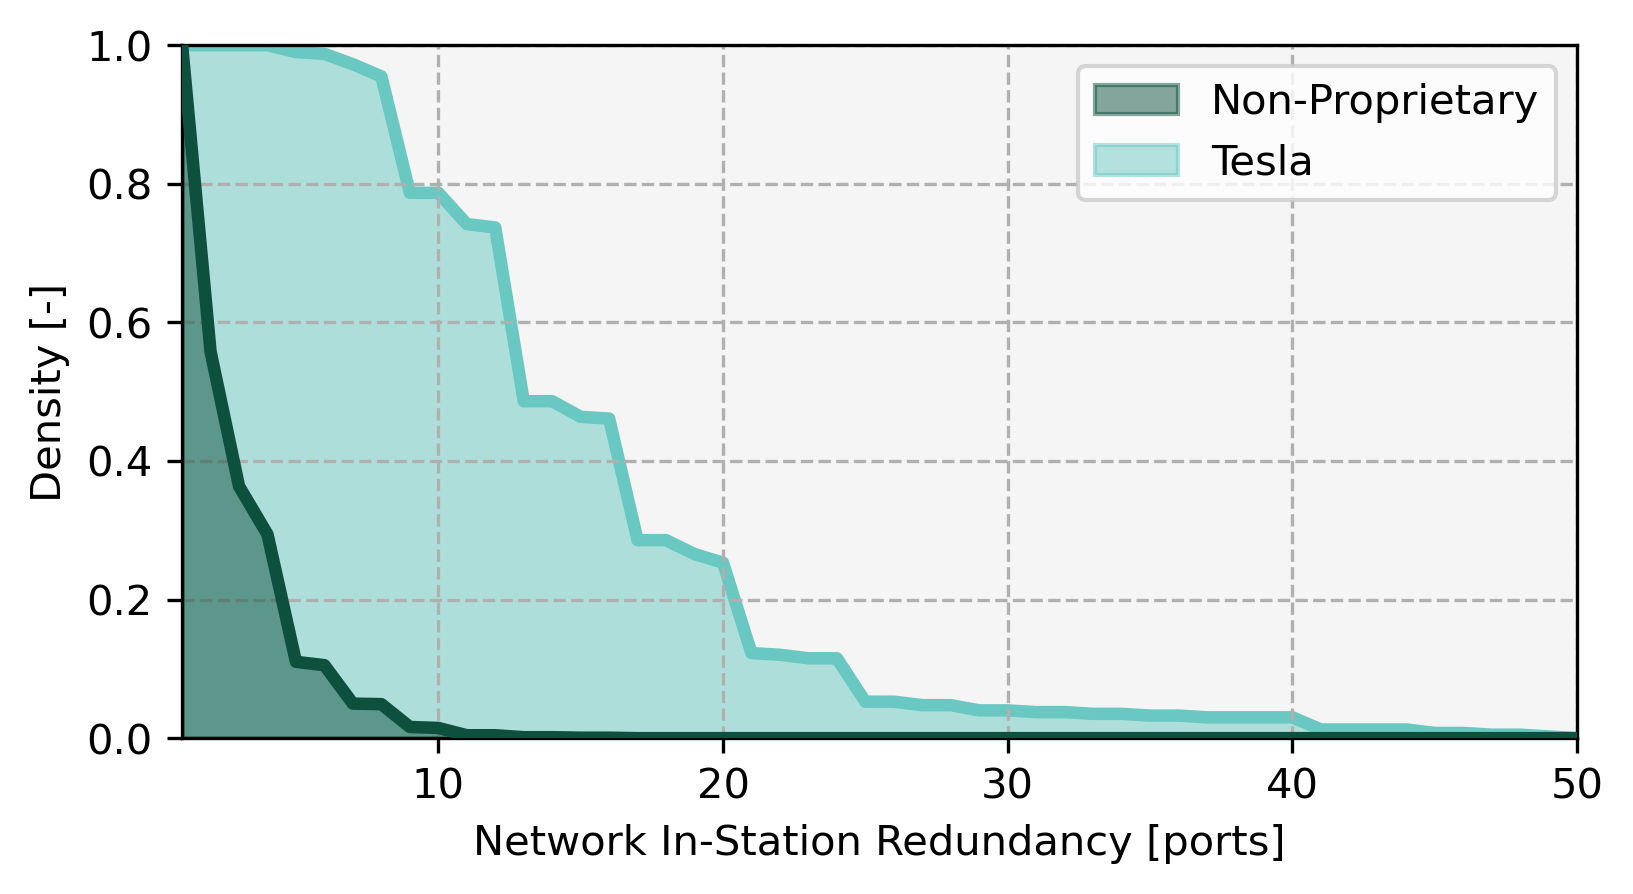
\includegraphics[width = \linewidth]{figs/California_RIS_Hist.png}
	\caption{Survival functions for in-station redundancy for Tesla and other DC charger networks in California}
	\label{fig:network_histograms}
\end{figure}

The Tesla DC charging network develops redundancy primarily in-station where the non-proprietary networks develop redundancy primarily between stations. Non-Tesla chargers are also more likely to be sighted in urban areas suggesting a desire to capture local as well as corridor travel demand. Tesla stations are more often sighted along travel corridors suggesting a focus on enabling long distance travel. In more remote parts of California the proprietary networks nearly match the non-proprietary networks in between-station redundancy. In-station and between-station redundancies for DC charging networks in California can be found in Figures [REF] and [REF] in the Appendix. Summary statistics for DC charging networks in California can be found in Tables [REF] and [REF] in the appendix.

California \glspl{icev} utilize a third and completely separate network of supply stations. There are estimated to be over 8,000 gasoline stations in California \cite{CEC_2022} and these are widely and proportionally distributed. Because no public database for the locations of gasoline stations in the state exists, and due to their ubiquity it is assumed in this study that \gls{icev} driver optimal paths will not be effected by fueling station availability. For this reason, \glspl{icev} are, herein, assumed to take the "direct" path between cities where \glspl{bev} need to find optimal paths on their \glspl{sng}.

\subsection*{Experiment}

In order to understand the effects of vehicular, infrastructural, and behavioral parameters on road-trip accessibility an experiment was carried out on randomly generated combinations. As a baseline, three \glspl{icev} were also modeled. These \glspl{icev} represent different levels of efficiency present in the present \gls{icev} fleet. \gls{ess} capacity numbers were pulled from manufacturer websites and energy consumption rates are computed from EPA highway fuel economy ratings \cite{DOE_EPA_2024}. Although substantially less efficient than equivalent \glspl{bev} the comparatively high specific energy of liquid petroleum allows for \glspl{icev} to have higher maximum ranges. \gls{icev} supply infrastructure is modeled to dispense fuel at the normal US rate of 7 gallons per minute which is an equivalent energy supply rate of 14.15 MW. When refueling, the Prius. Golf, and Pacifica, add highway range at rates of 631, 462, and 282 km per minute. respectively. The \gls{icev} model data and California road-trip accessibility vales are shown in Table \ref{tab:icev_models}.

\begin{table}[H]
	\centering
	\caption{\gls{icev} models}
	\label{tab:icev_models}
	\begin{tabular}{|C{.45\linewidth}|C{.3\linewidth}|C{.25\linewidth}|}
		\hline Vehicle Model & Parameter & Value \\
		\cline{1-3} & \gls{ess} Capacity & 381 [kWh] \\
		\cline{2-3} & Energy Consumption & 1,346 [kJ/km] \\
		\cline{2-3} 2024 Toyota Prius & Full-Tank Range & 1,018 [km] \\
		\cline{2-3} & California Road-Trip Accessibility & 5.472 [hours] \\
		\cline{1-3} & \gls{ess} Capacity & 445 [kWh] \\
		\cline{2-3} & Energy Consumption & 1,839 [kJ/km] \\
		\cline{2-3} 2024 Volkswagen Golf & Full-Tank Range & 871 [km] \\
		\cline{2-3} & California Road-Trip Accessibility & 5.492 [hours] \\
		\cline{1-3} & \gls{ess} Capacity & 640 [kWh] \\
		\cline{2-3} & Energy Consumption & 3,015 [kJ/kM] \\
		\cline{2-3} 2024 Chrysler Pacifica & Full-Tank Range & 764 [km] \\
		\cline{2-3} & California Road-Trip Accessibility & 5.517 [hours] \\
		\hline
	\end{tabular}
\end{table}

Road-trip accessibility for \glspl{icev} was computed under the assumption of petroleum supply infrastructure ubiquity. As such, \glspl{icev} were given the "direct" path between locations with stop times added where additional range was needed. For each necessary stop, time was added for refueling to full as well as 10 minutes to divert from the road and handle the transaction prior to refueling. Additionally, drivers of the \glspl{icev} were assumed to keep a 10\% buffer of remaining range. The \glspl{icev} each had similar road-trip accessibility scores of roughly 5.5 hours. The longest arc considered in Crescent City (Location 0) to Phoenix - State Line (Location 13) which is roughly 1,530 km just exceeding double the usable range of the Pacifica. The Prius, Golf, and Pacifica required averages of 0.43, 0.31, and 0.19 supply stops per route respectively.

500 random scenarios were generated by uniform random sampling of the parameters listed in Table \ref{tab:experimental_parameters} and run on three \glspl{sng} as described in \ref{tab:experimental_sngs}. All randomly sampled \glspl{bev} in this study are assumed to have an energy consumption rate of 608 kJ/km this being the EPA energy consumption rate of a Tesla Model 3 in highway operation \cite{DOE_EPA_2024}. Highway operation is assumed herein due to the focus on long trips. Thus \gls{bev} full-charge ranges will be between 237 and 711 km. Vehicles are assumed to fast charge only up to 80\% \gls{soc} in order to remain in the constant current range. When charging, sampled \glspl{bev} add highway range at a rate between 4.9 and 19.7 km per minute. Risk attitude was modeled as in \eqref{eq:superquantile} with the range centered around the mean parameter $\overline{p}$ where $p_0 = \overline{p} - .1$ and $p_1 = \overline{p} + .1$. 

\begin{table}[H]
	\centering
	\caption{Parameters and ranges for experiment.}
	\label{tab:experimental_parameters}
	\begin{tabular}{|C{\linewidth/2}|C{\linewidth/2}|}
		\hline Parameter & Range \\
		\hline \gls{ess} Capacity & [40 kWh, 120 kWh] \\
		\hline \gls{ess} Max Charge Rate & [50 kW, 200 kW] \\
		\hline Driver Risk-Attitude Mean & [.1, .9] \\
		\hline \gls{evse} Reliability & [.5, 1] \\
		\hline Station Arrival Ratio Mean & [1, 3] \\
		\hline
	\end{tabular}
\end{table}

\begin{table}[H]
	\centering
	\caption{\glspl{sng} used in experiment.}
	\label{tab:experimental_sngs}
	\begin{tabular}{|C{\linewidth/3}|C{\linewidth*2/3}|}
		\hline Label & Networks Included \\
		\hline Combined & All stations \\
		\hline Tesla & Only Tesla stations \\
		\hline Non-Tesla & All non-Tesla stations \\
		\hline
	\end{tabular}
\end{table}

The parameter levels chosen were based on ...

Linear regression was performed on the results of the random experiment. Using as output, the neutral expectation of road-trip accessibility for each of the 500 randomly sampled vehicles on each of the \glspl{sng}. Significant parameters from the regression are shown in Figure \ref{fig:significant_parameters}.

\begin{figure}[H]
	\centering
	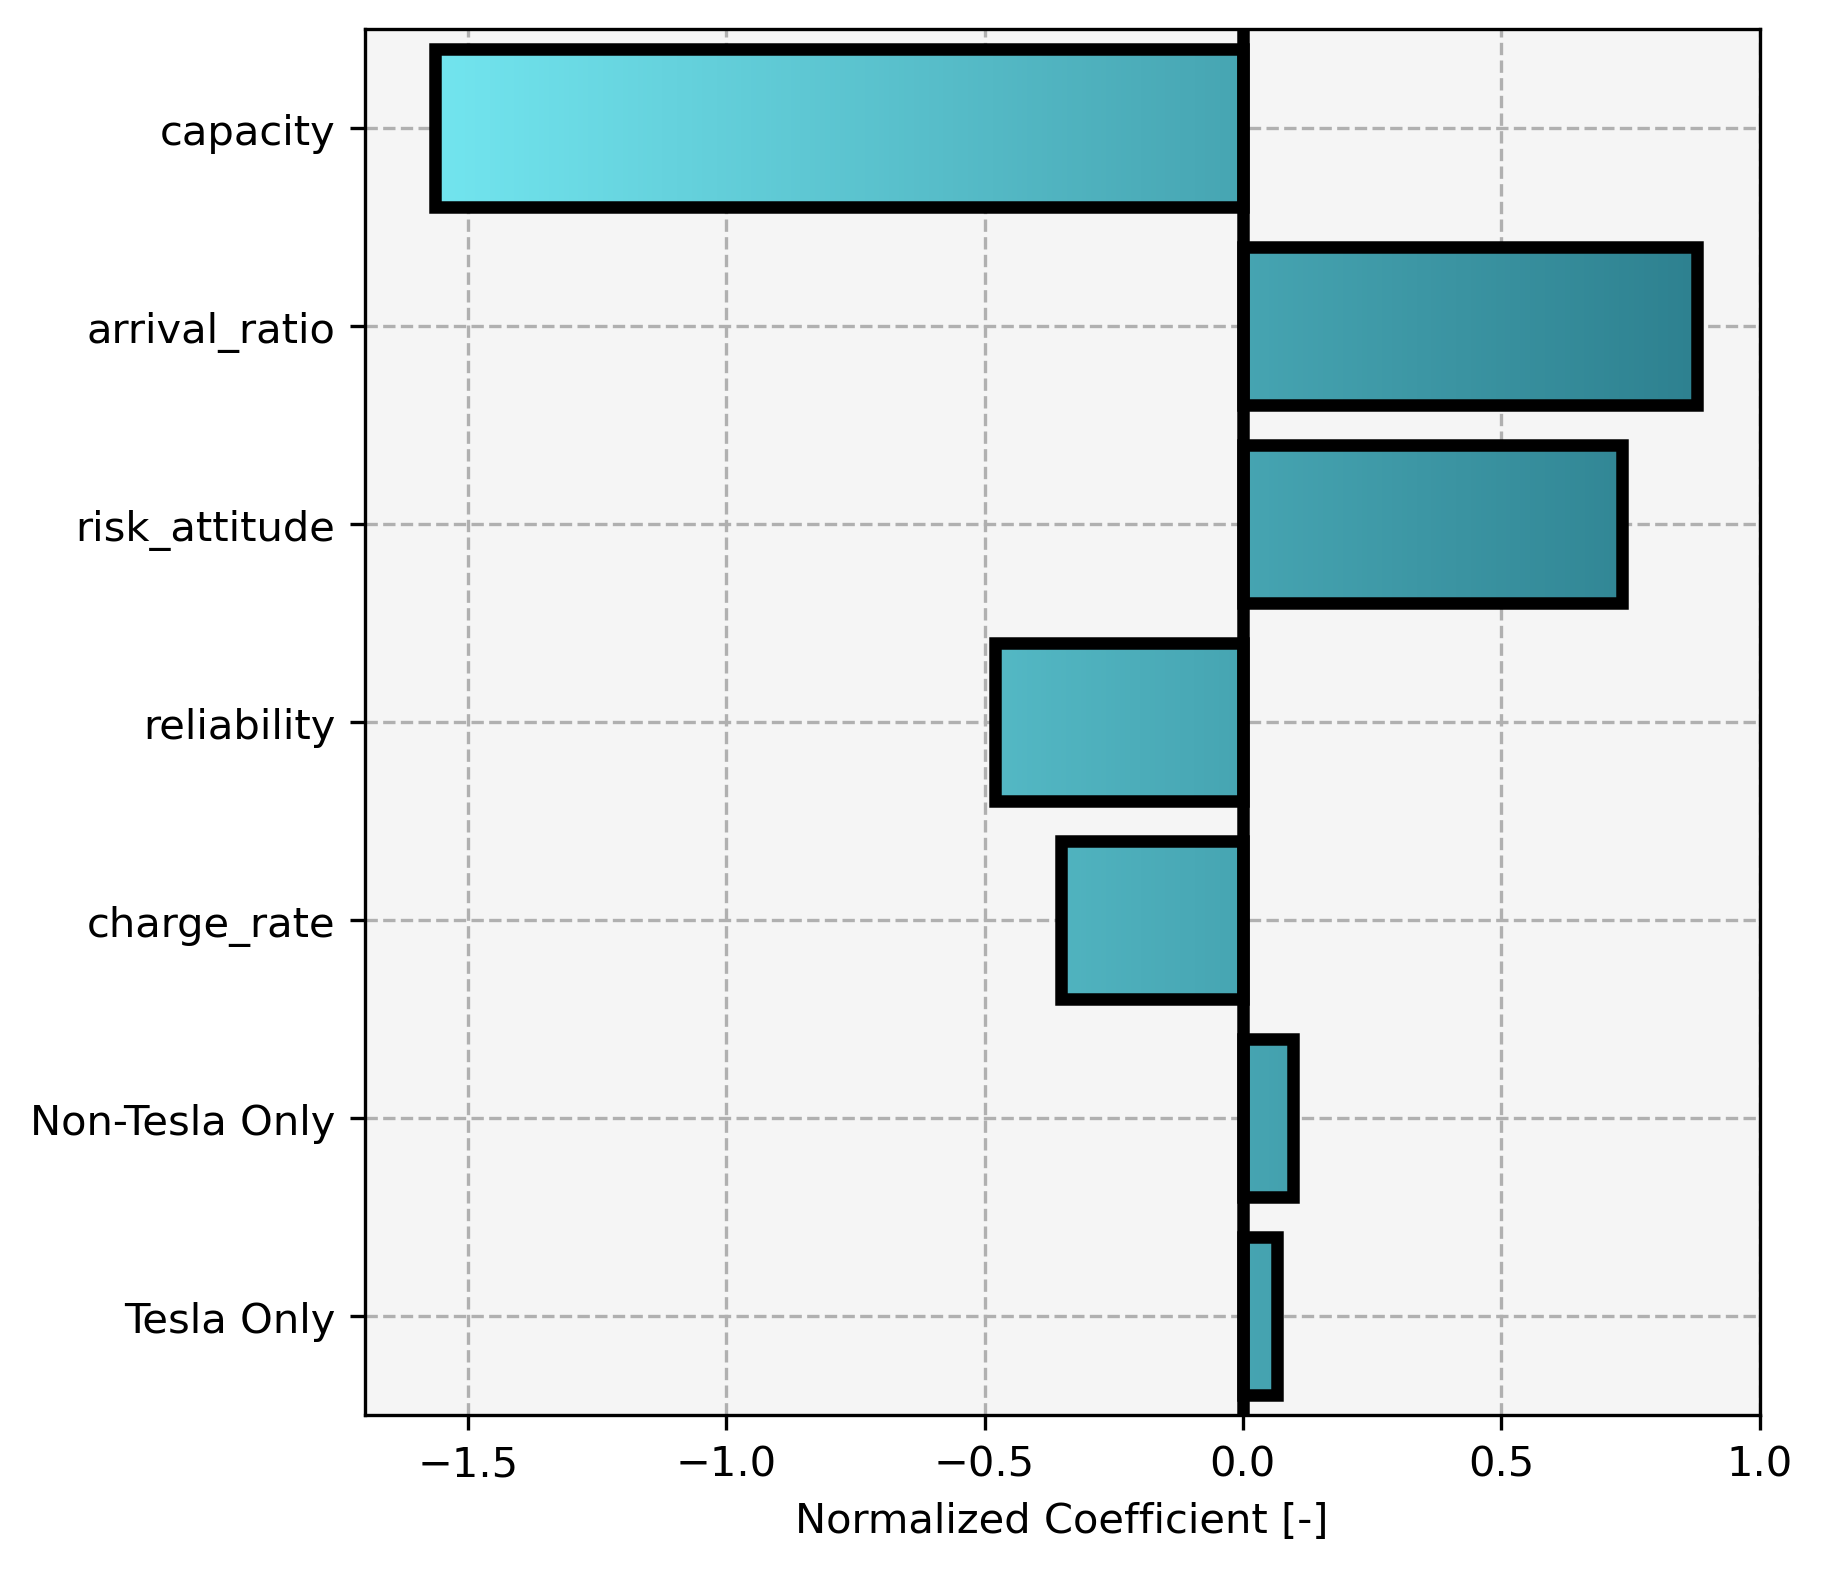
\includegraphics[width = \linewidth]{figs/significant_parameters.png}
	\caption{Coefficients for significant parameters from linear regression}
	\label{fig:significant_parameters}
\end{figure}

Regression details are provided in Tables [REF] and [REF] in the Appendix. The regression analysis shows that vehicular, infrastructural, and behavioral parameters have significant impacts on road-trip accessibility. The vehicular parameters of capacity and charge rate have the predictable effect of reducing expected travel times. Capacity being the more more important parameter is explicable as higher capacity vehicles offer the ability to stop less frequently. Saving an entire charging event can be very impactful in a region the size of California. Among the infrastructure parameters, higher reliability contributed to lower travel times where higher arrival ratios contributed to higher travel times. Both reliability and arrival ratio primarily effect queuing times as, even with 50\% equipment reliability, most stations have sufficient redundancy to guarantee at least one operational charger. The range of arrivals ratios considered goes from normal to swamped and long queues can be expected for high arrival ratios even at high redundancy stations. Risk attitude was also significant in determining outcomes as those drivers with more cautious risk attitudes will tend to maintain higher \gls{soc} and utilize more reliable and redundant routes. finally, access to the entire network is better than restriction to just part of it but being restricted to only Tesla stations should be slightly less damaging than access to only non-Tesla stations. Boxplots of expected travel times are shown in Figure \ref{fig:networks_boxplots}.

\begin{figure}[H]
	\centering
	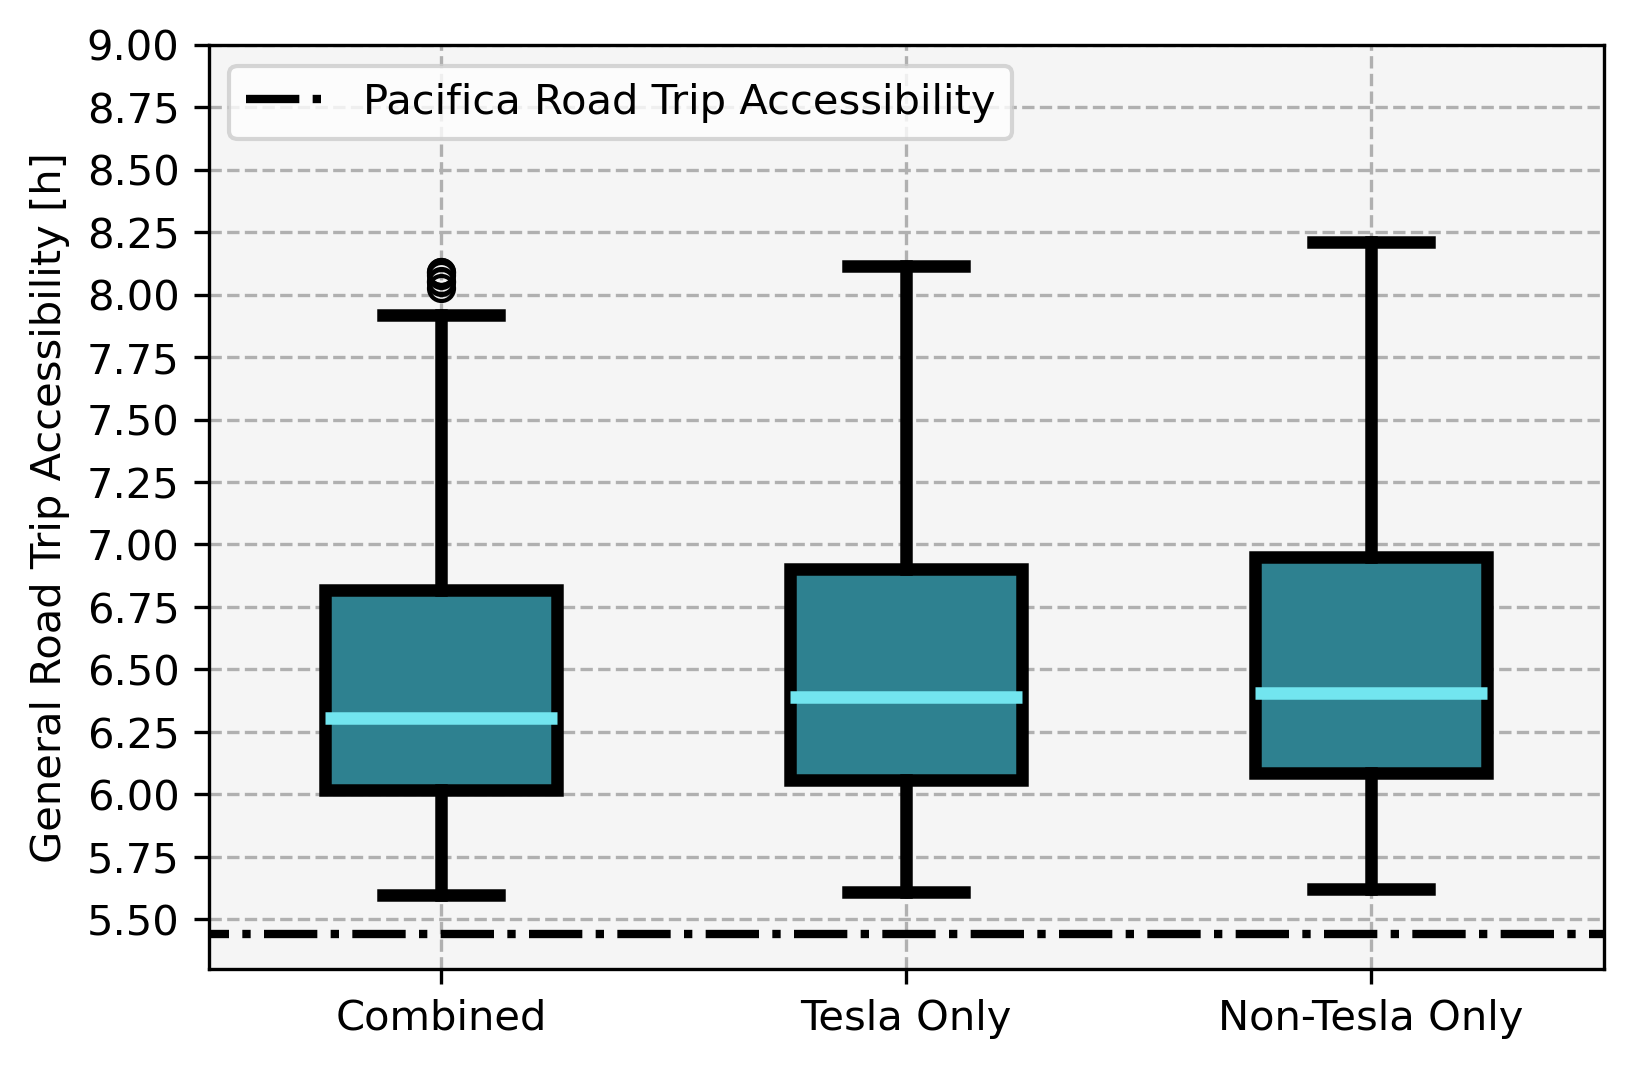
\includegraphics[width = \linewidth]{figs/Networks_Boxplots_RTA.png}
	\caption{Boxplots of experiment outputs by \gls{sng}}
	\label{fig:networks_boxplots}
\end{figure}

While the differences between the \glspl{bev} on the basis of \gls{sng} access are observed to be slight, the differences between the means of each and the worst of the \glspl{icev} is quite large. The difference is roughly 45 minutes much of which can be explained by the shorter ranges and longer supply times inherent to the \glspl{bev}. Isolating the driving times by subtracting supply and setup times, the differences between the vehicles and \glspl{sng} are substantially smaller as shown in Figure \ref{fig:networks_boxplots_driving}.

\begin{figure}[H]
	\centering
	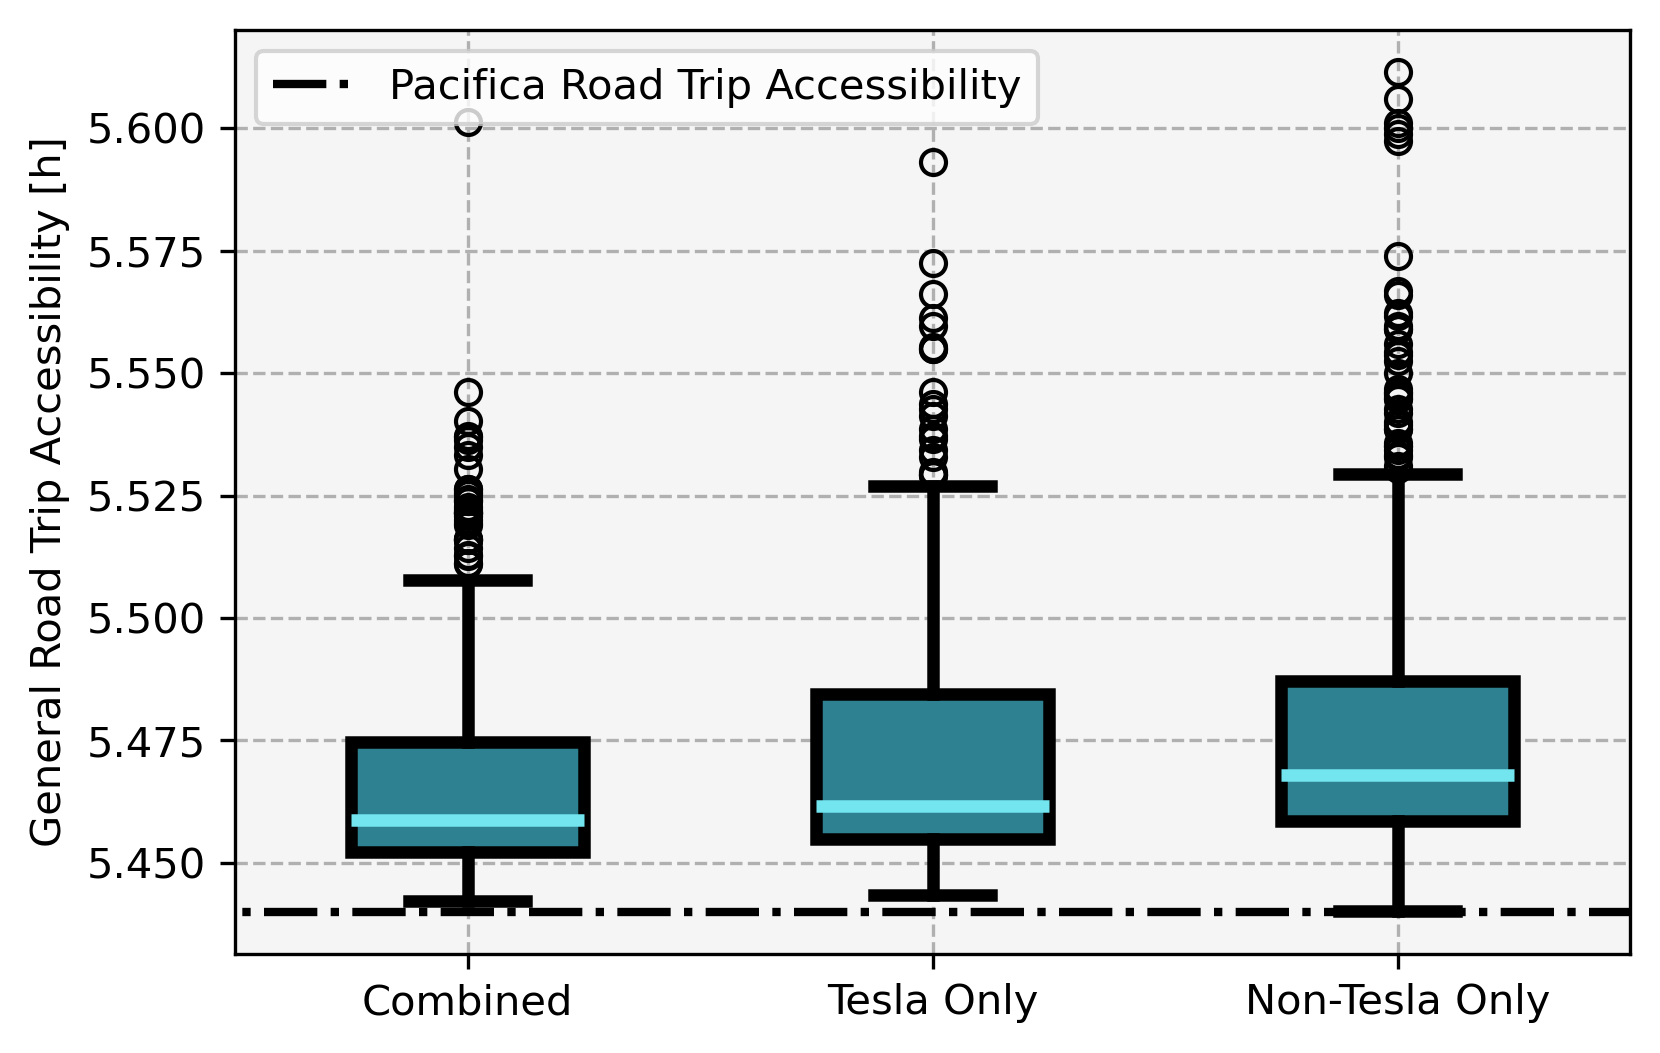
\includegraphics[width = \linewidth]{figs/Networks_Boxplots_RTA_D.png}
	\caption{Boxplots of experiment outputs by \gls{sng} (driving time only)}
	\label{fig:networks_boxplots_driving}
\end{figure}

The optimal routes generated in this study only selected corridor chargers. Some insight into the utility provided by each network can be gained by looking into utilization rates for each of the networks as seen in Figure \ref{fig:utilization_rates}.

\begin{figure}[H]
	\centering
	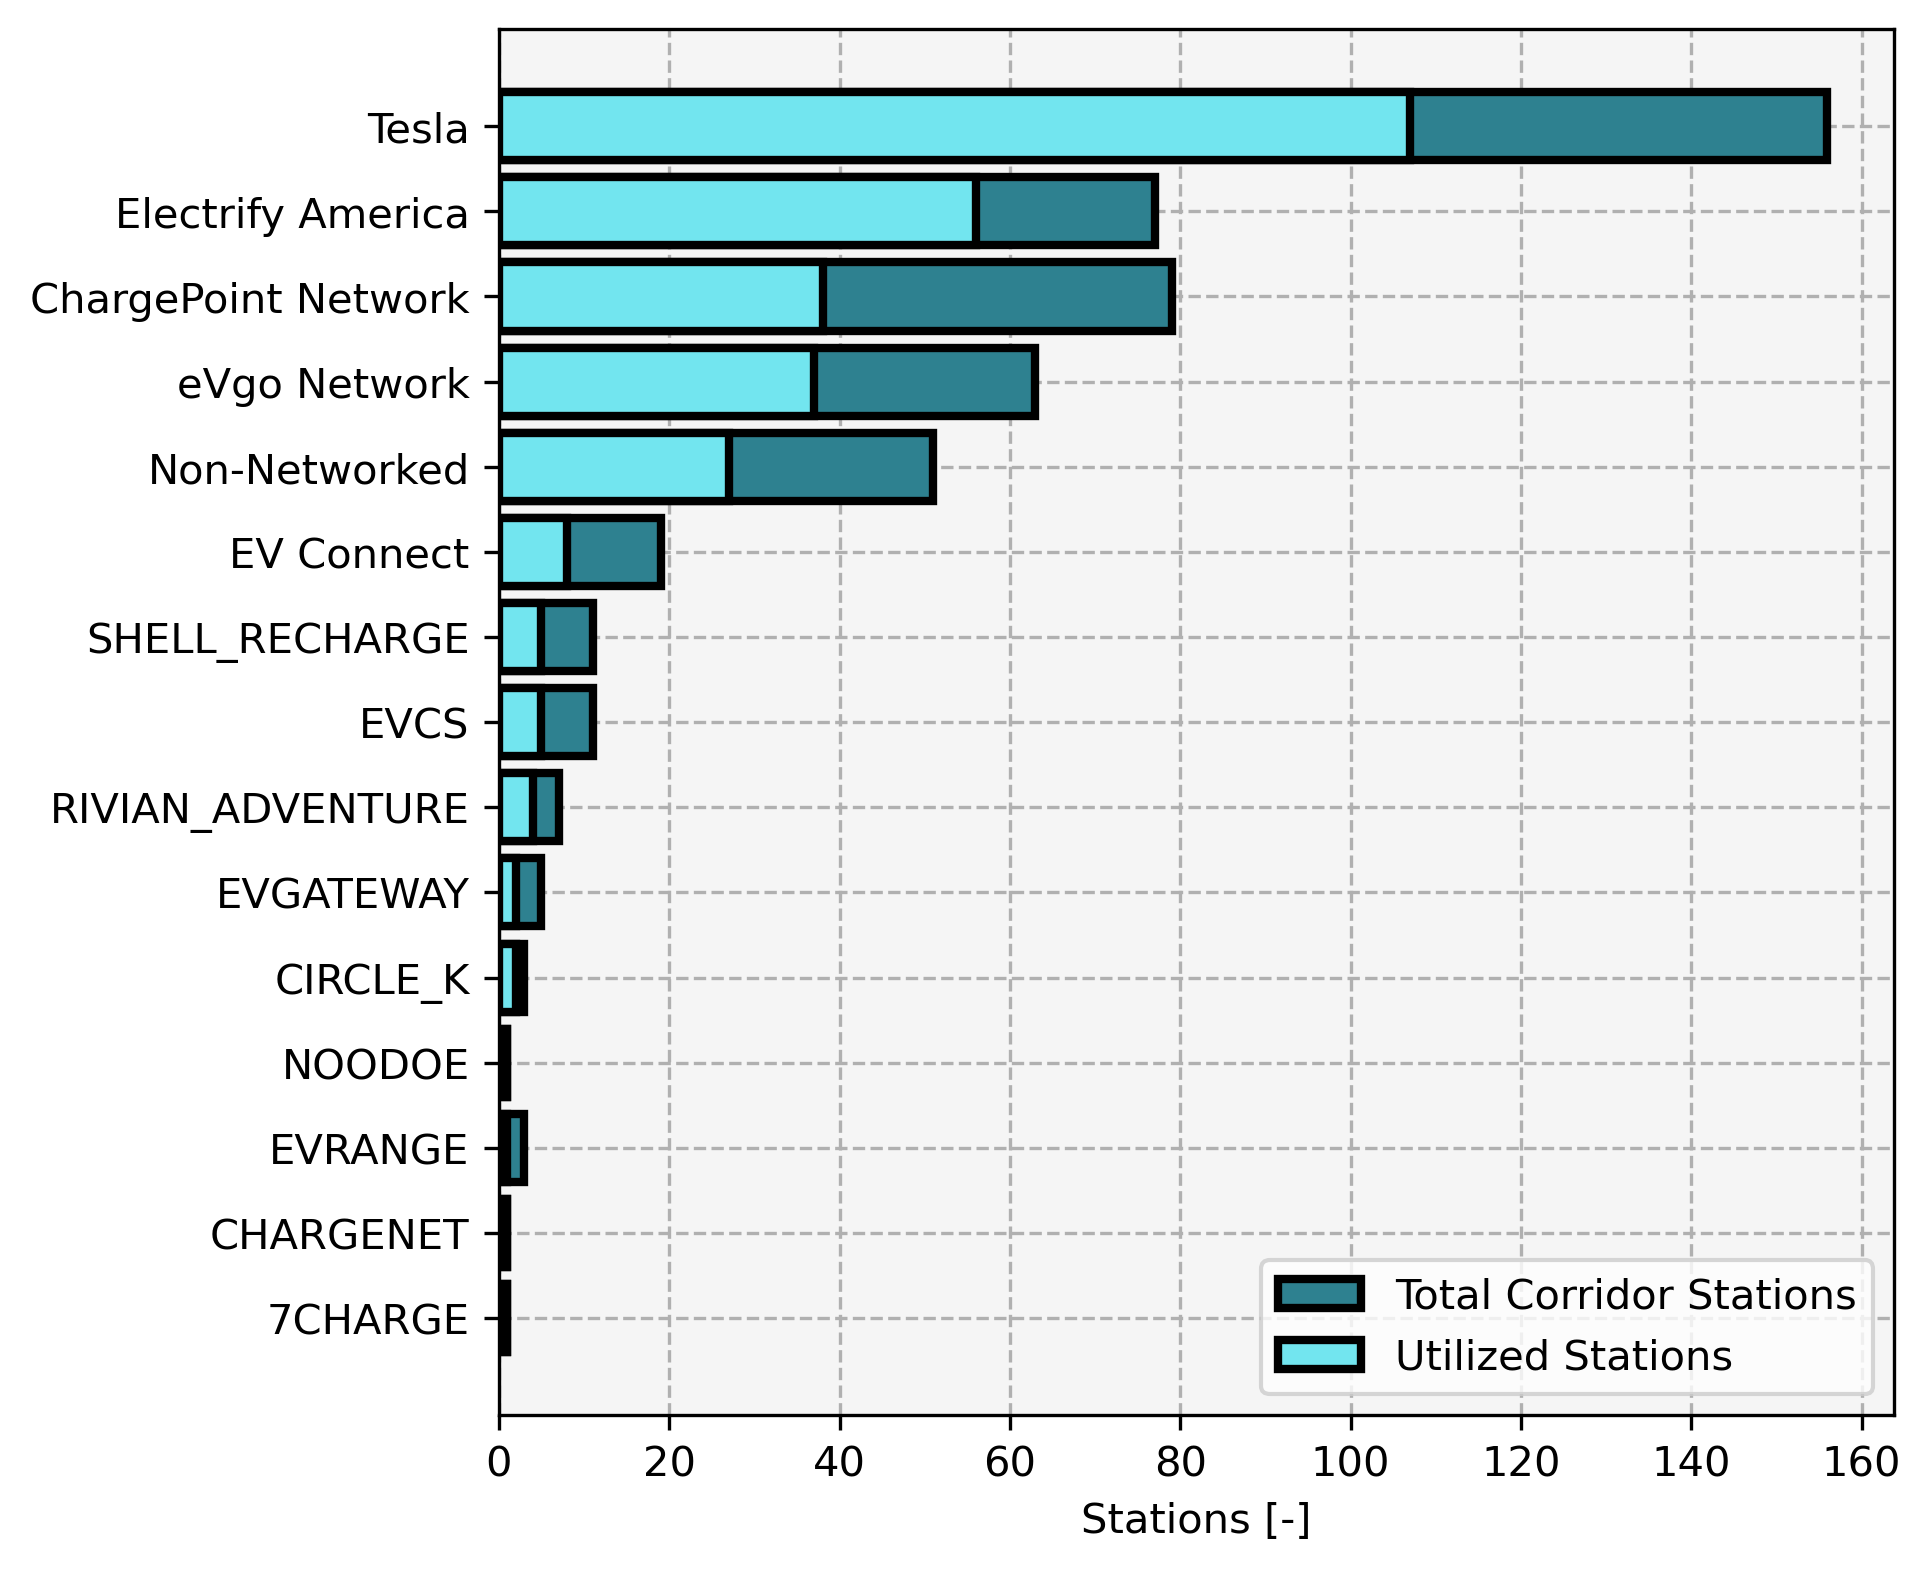
\includegraphics[width = \linewidth]{figs/corridor_station_utilization.png}
	\caption{Corridor DC charging network utilization rates}
	\label{fig:utilization_rates}
\end{figure}


Also include a figure showing locations of utilized vs. non-utilized chargers. Mention that this really only reflects on location and composition and that real differences in equipment reliability are not factored in.



This study focuses on travel times and routing did not optimize for energy cost. At present there is no publicly available data on energy costs at a granular station-level for either gasoline or DC fast charging stations. Nevertheless, some sense of the relative economics of long-trip travel can be attained by examining energy costs per km. Conventional wisdom suggests that \glspl{bev} should offer a potential cost savings on the basis of average energy costs. Energy costs vary substantially by region in the US with California being the most expensive. Energy costs around the time of writing are shown in Table \ref{tab:energy_costs}.

\begin{table}[H]
	\centering
	\caption{Residential electricity and petroleum average prices USD}
	\label{tab:energy_costs}
	\begin{tabular}{|C{.31\linewidth}|C{.23\linewidth}|C{.23\linewidth}|C{.23\linewidth}|}
		\hline Source & US & California & Percentage Increase \\
		\hline Petroleum [gallon] & 3.609 & 5.138 & 42.37 \\
		\hline Residential Electricity [kWh] & 0.1668 & 0.3247 & 94.66 \\
		\hline Transportation Electricity [kWh] & 0.1520 & 0.1191 & 27.62 \\
		\hline DC Fast Charging (Estimated) [kWh] & 0.35 - 0.50 & 0.35 - 0.60 & 0 - 20 \\
		\hline
	\end{tabular}
\end{table}

Petroleum prices are from AAA \cite{AAA_2024} and energy prices are from EIA \cite{EIA_2024}. DC fast charging pricing schemes display much heterogeneity and may not be as easily accounted as metered electricity prices. An Ad-Hoc Text Mining study performed on over 90,000 recorded PlugShare events from 2019 and 2021 found the mode of DC fast charging prices to be in the range of 0.3 and 0.4 USD per kWh \cite{Trinko_2021}. Prices did not significantly correlate with local energy prices. In the same time period California residential electricity increased from 0.1995 USD per kWh to 0.2282 USD per kWh and transportation electricity increased from 0.0891 to 0.1179 USD per kWh. By comparison with 2024 electricity prices, one would expect prices in the range of 0.35 and 0.60 USD per kWh for DC fast charging in California and 0.35 to 0.5 in the US, ranges backed by informal reporting \cite{CalTrans_2024, Sowder_2024}. Thus, expected energy costs per highway km traveled can be computed and are shown in Table \ref{tab:expected_energy_costs_per_km}.

\begin{table}[H]
	\centering
	\caption{Expected energy costs per highway km traveled in US cents.}
	\label{tab:expected_energy_costs_per_km}
	\begin{tabular}{|C{\linewidth / 4}|C{\linewidth / 4}|C{\linewidth / 4}|C{\linewidth / 4}|}
		\hline Vehicle & Source & US Price & CA Price \\
		\hline Prius & Petroleum & 4.00 & 5.70 \\
		\hline Golf & Petroleum & 5.47 & 7.78 \\
		\hline Pacifica & Petroleum & 8.97 & 12.77 \\
		\hline \gls{bev} & Residential Electricity & 2.82 & 5.48 \\
		\hline \gls{bev} & DC Fast Charging & 5.91 - 8.44 & 5.91 - 10.13 \\
		\hline
	\end{tabular}
\end{table}

The economic picture is that, broadly speaking, DC fast charging a \gls{bev} presents no appreciable economic benefit over fueling an efficient \gls{icev}. In much of the US, home-charging a \gls{bev} provides cost savings for the initial part of the trip until supply is needed but this is not the case in California where residential electricity is, on average, nearly twice as expensive as the US average.




 

\newpage

\printbibliography

\appendix

\begin{figure}[H]
	\centering
	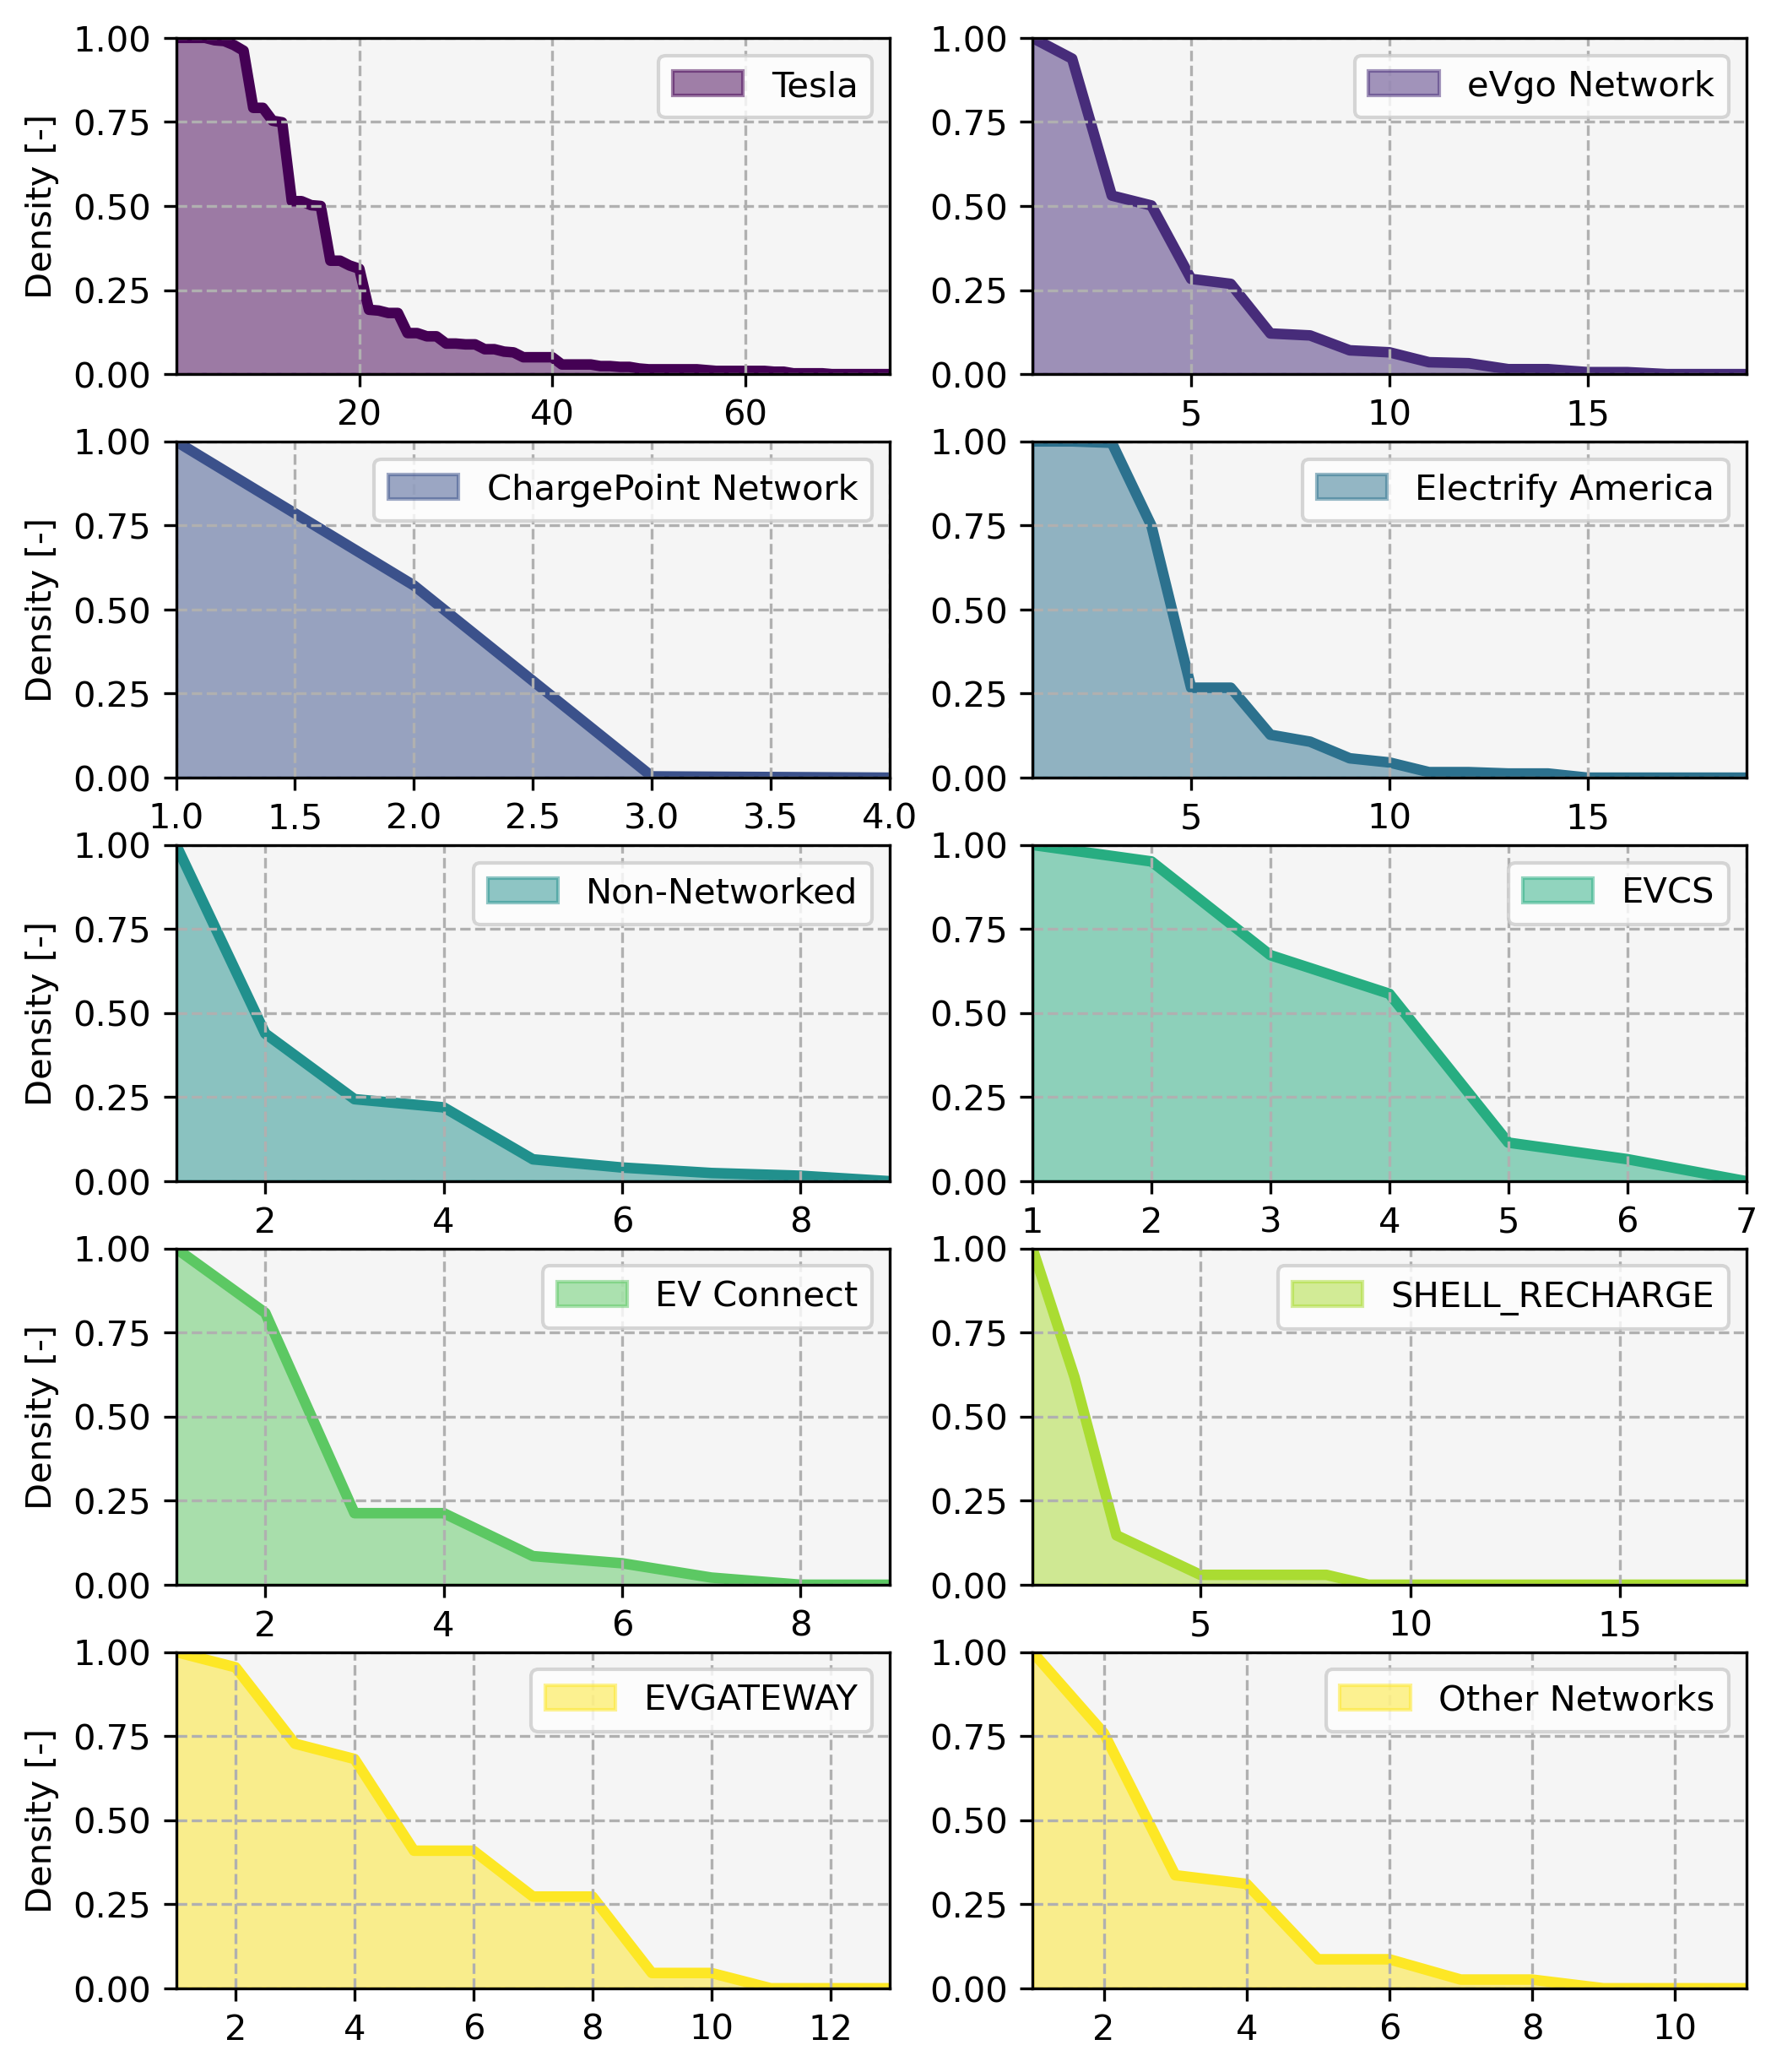
\includegraphics[width = \linewidth]{figs/California_RIS_SF_All.png}
	\caption{In-station redundancy for DC Charging networks in California}
	\label{fig:ris_top_networks}
\end{figure}

\begin{figure}[H]
	\centering
	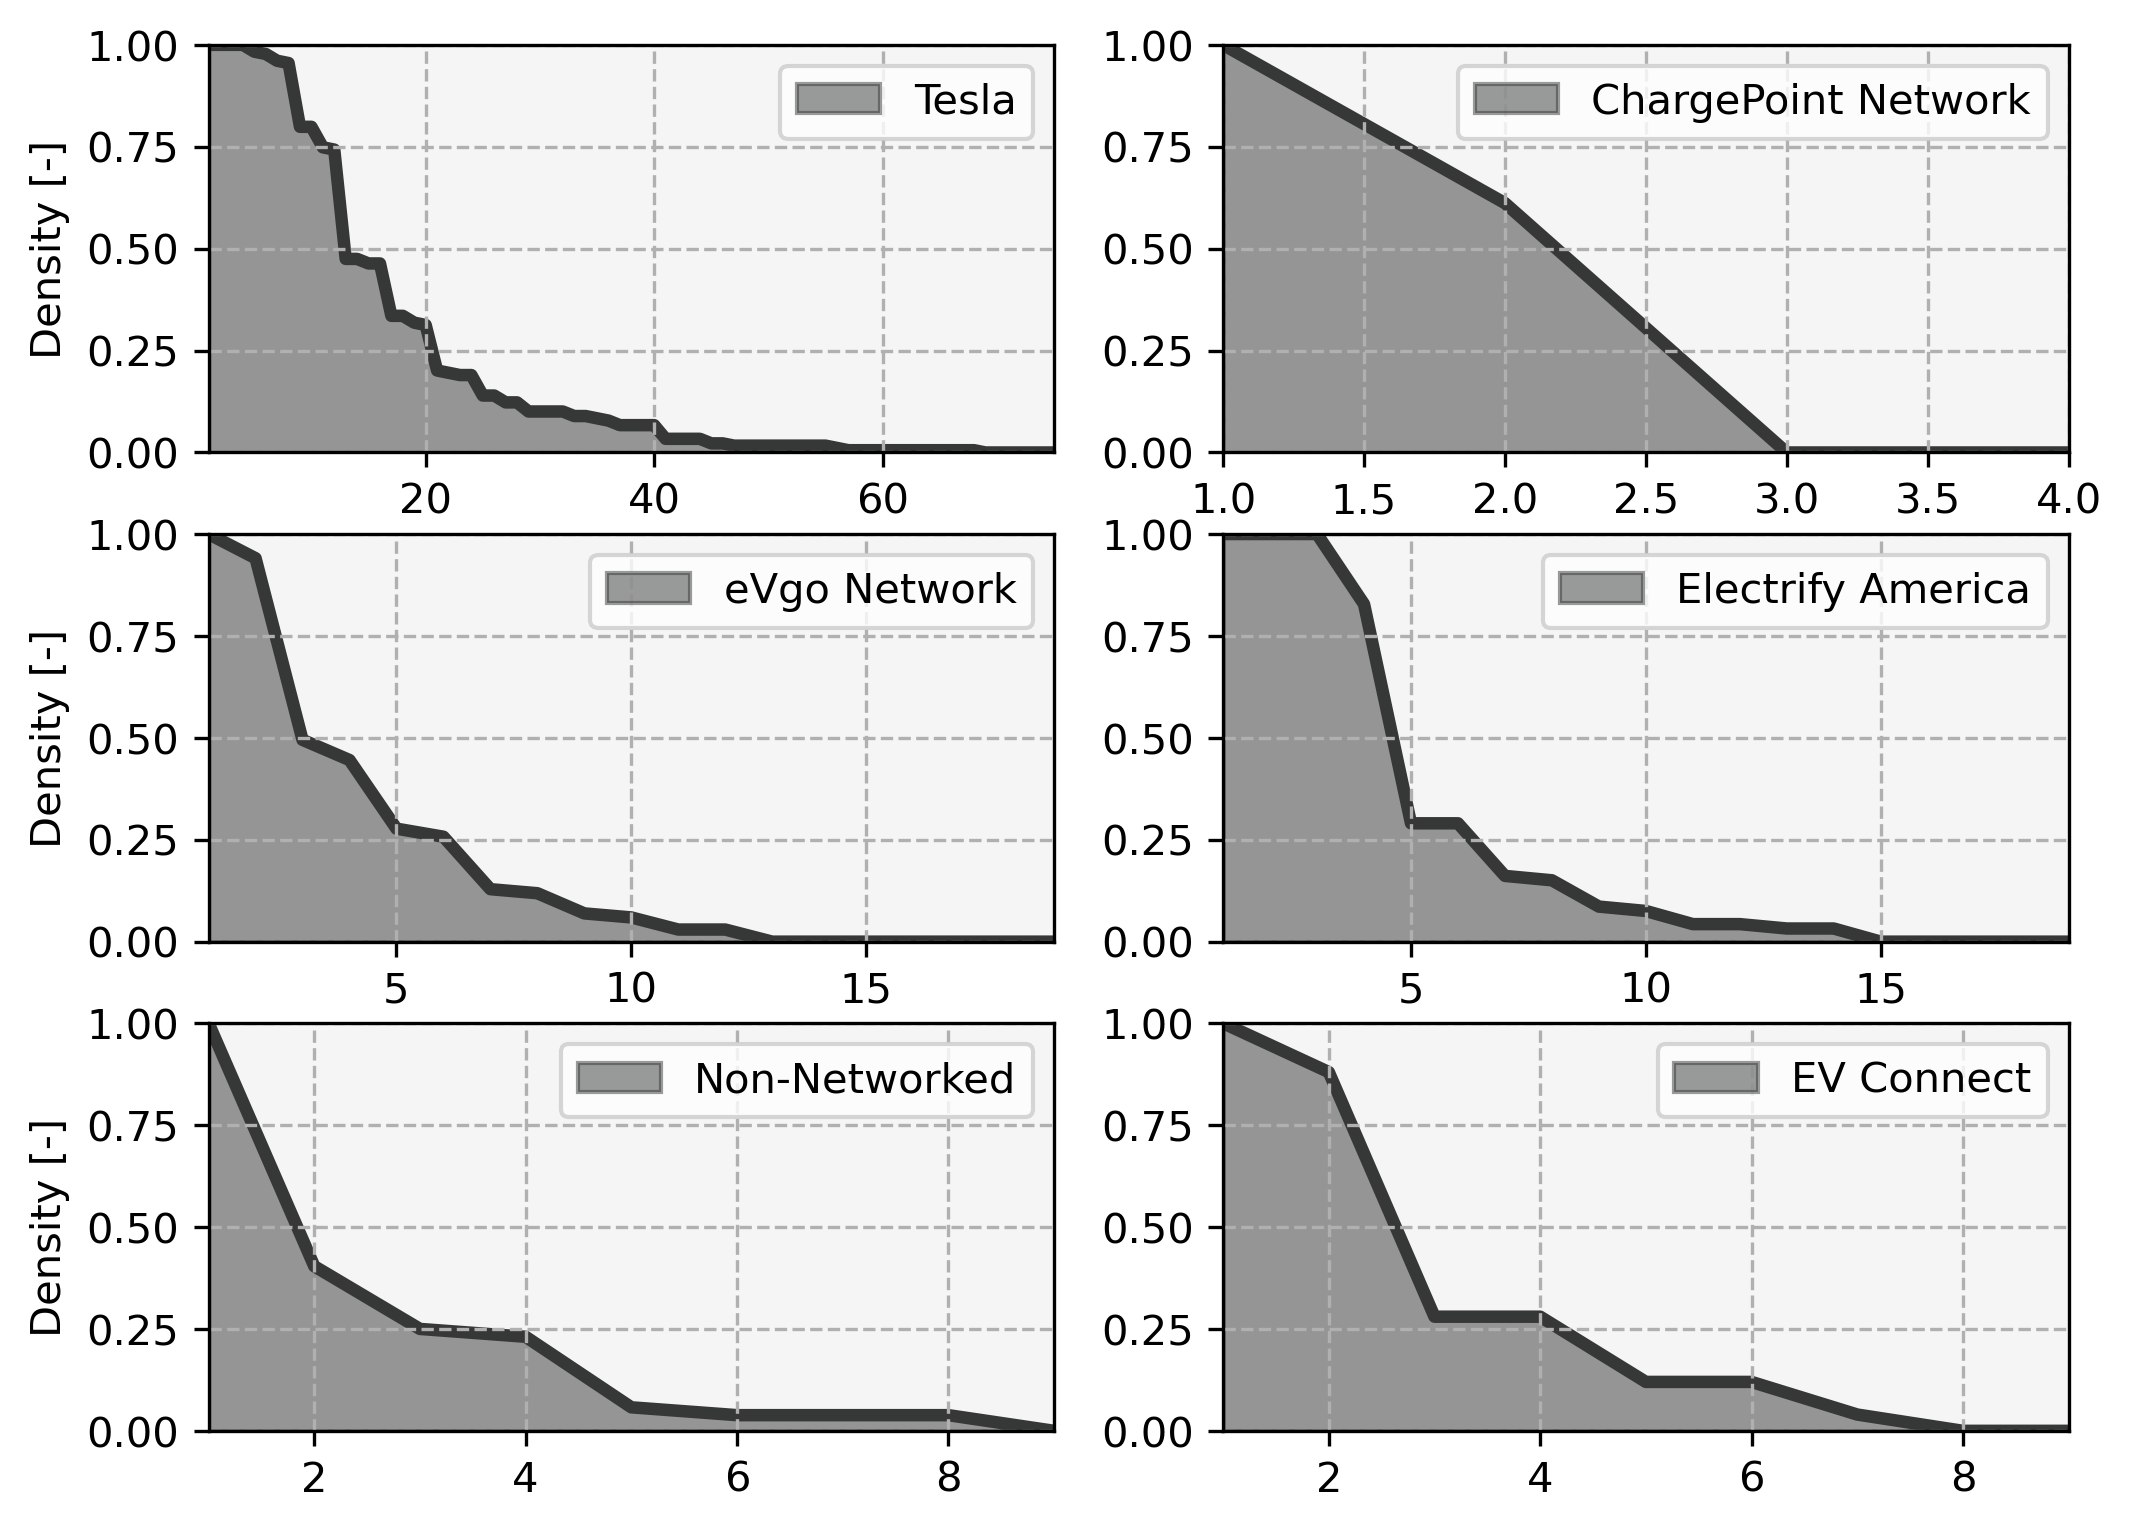
\includegraphics[width = \linewidth]{figs/California_RIS_SF_Corridor.png}
	\caption{In-station redundancy for DC Charging networks in California}
	\label{fig:ris_top_networks_corridor}
\end{figure}


%\begin{figure}[H]
%	\centering
%	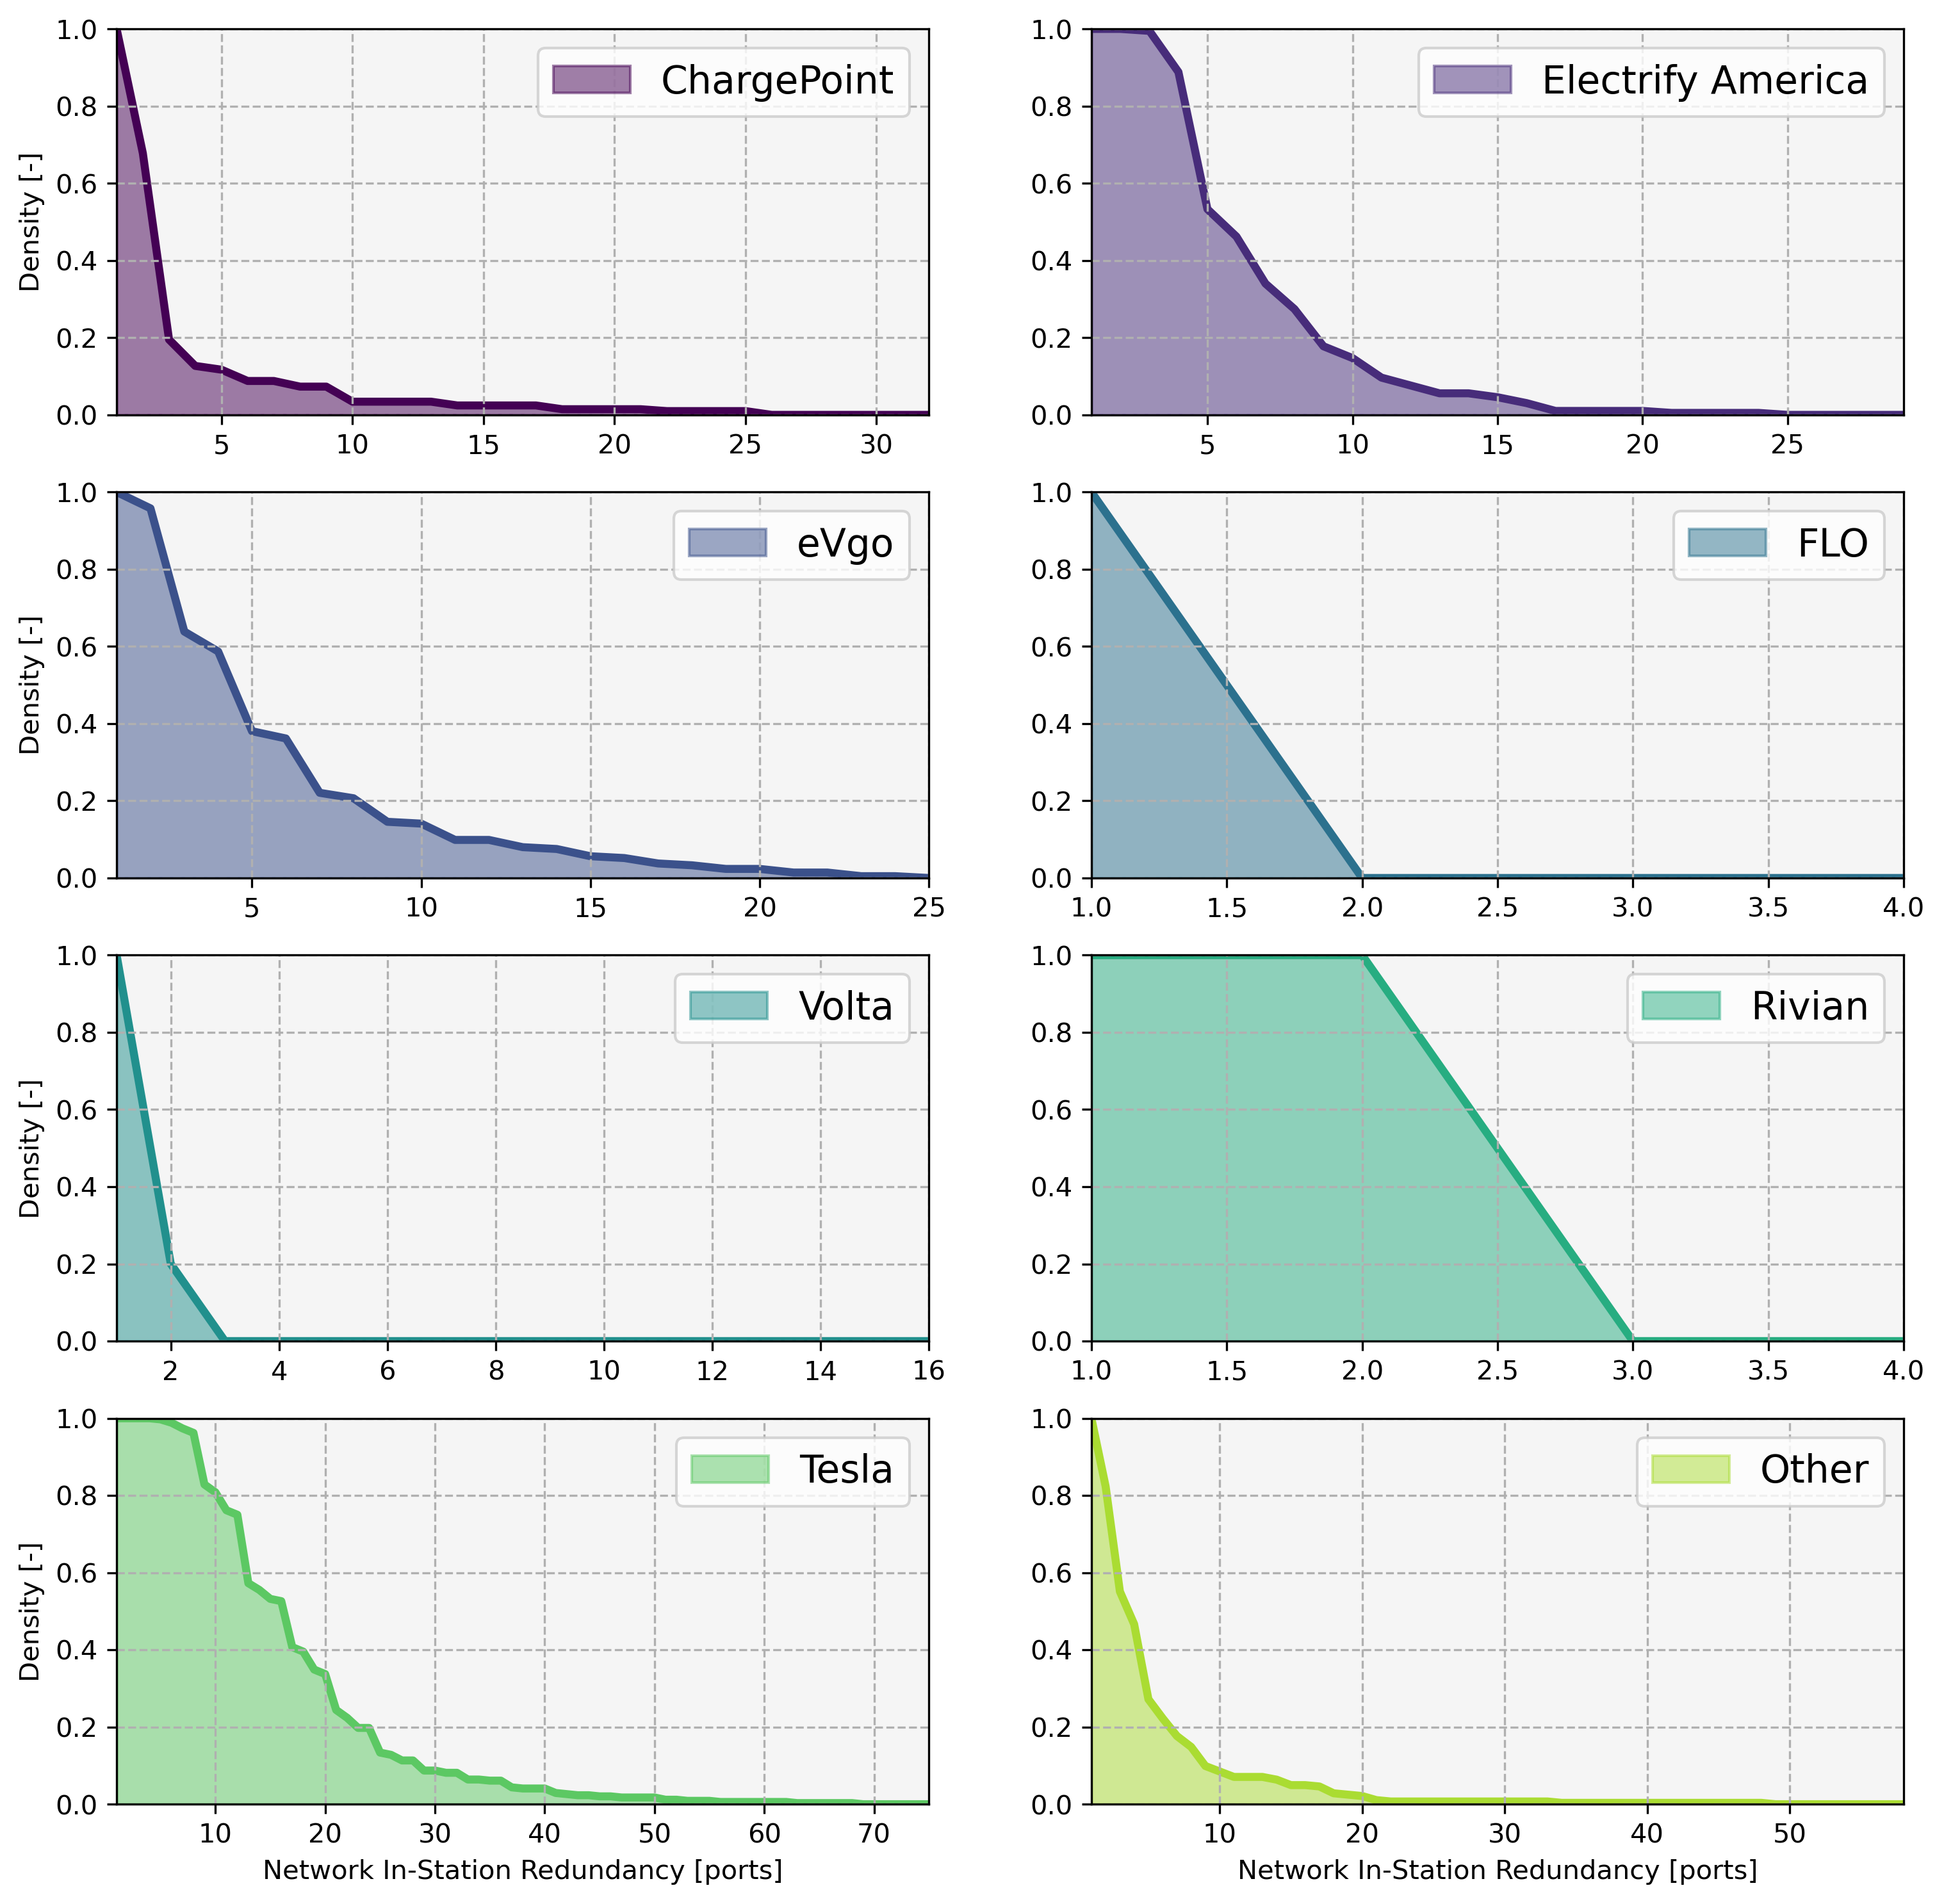
\includegraphics[width = \linewidth]{figs/California_RBS_300_SF_All.png}
%	\caption{In-station redundancy for DC Charging networks in California}
%	\label{fig:rbs_300_top_8_networks}
%\end{figure}
%
%
%\begin{figure}[H]
%	\centering
%	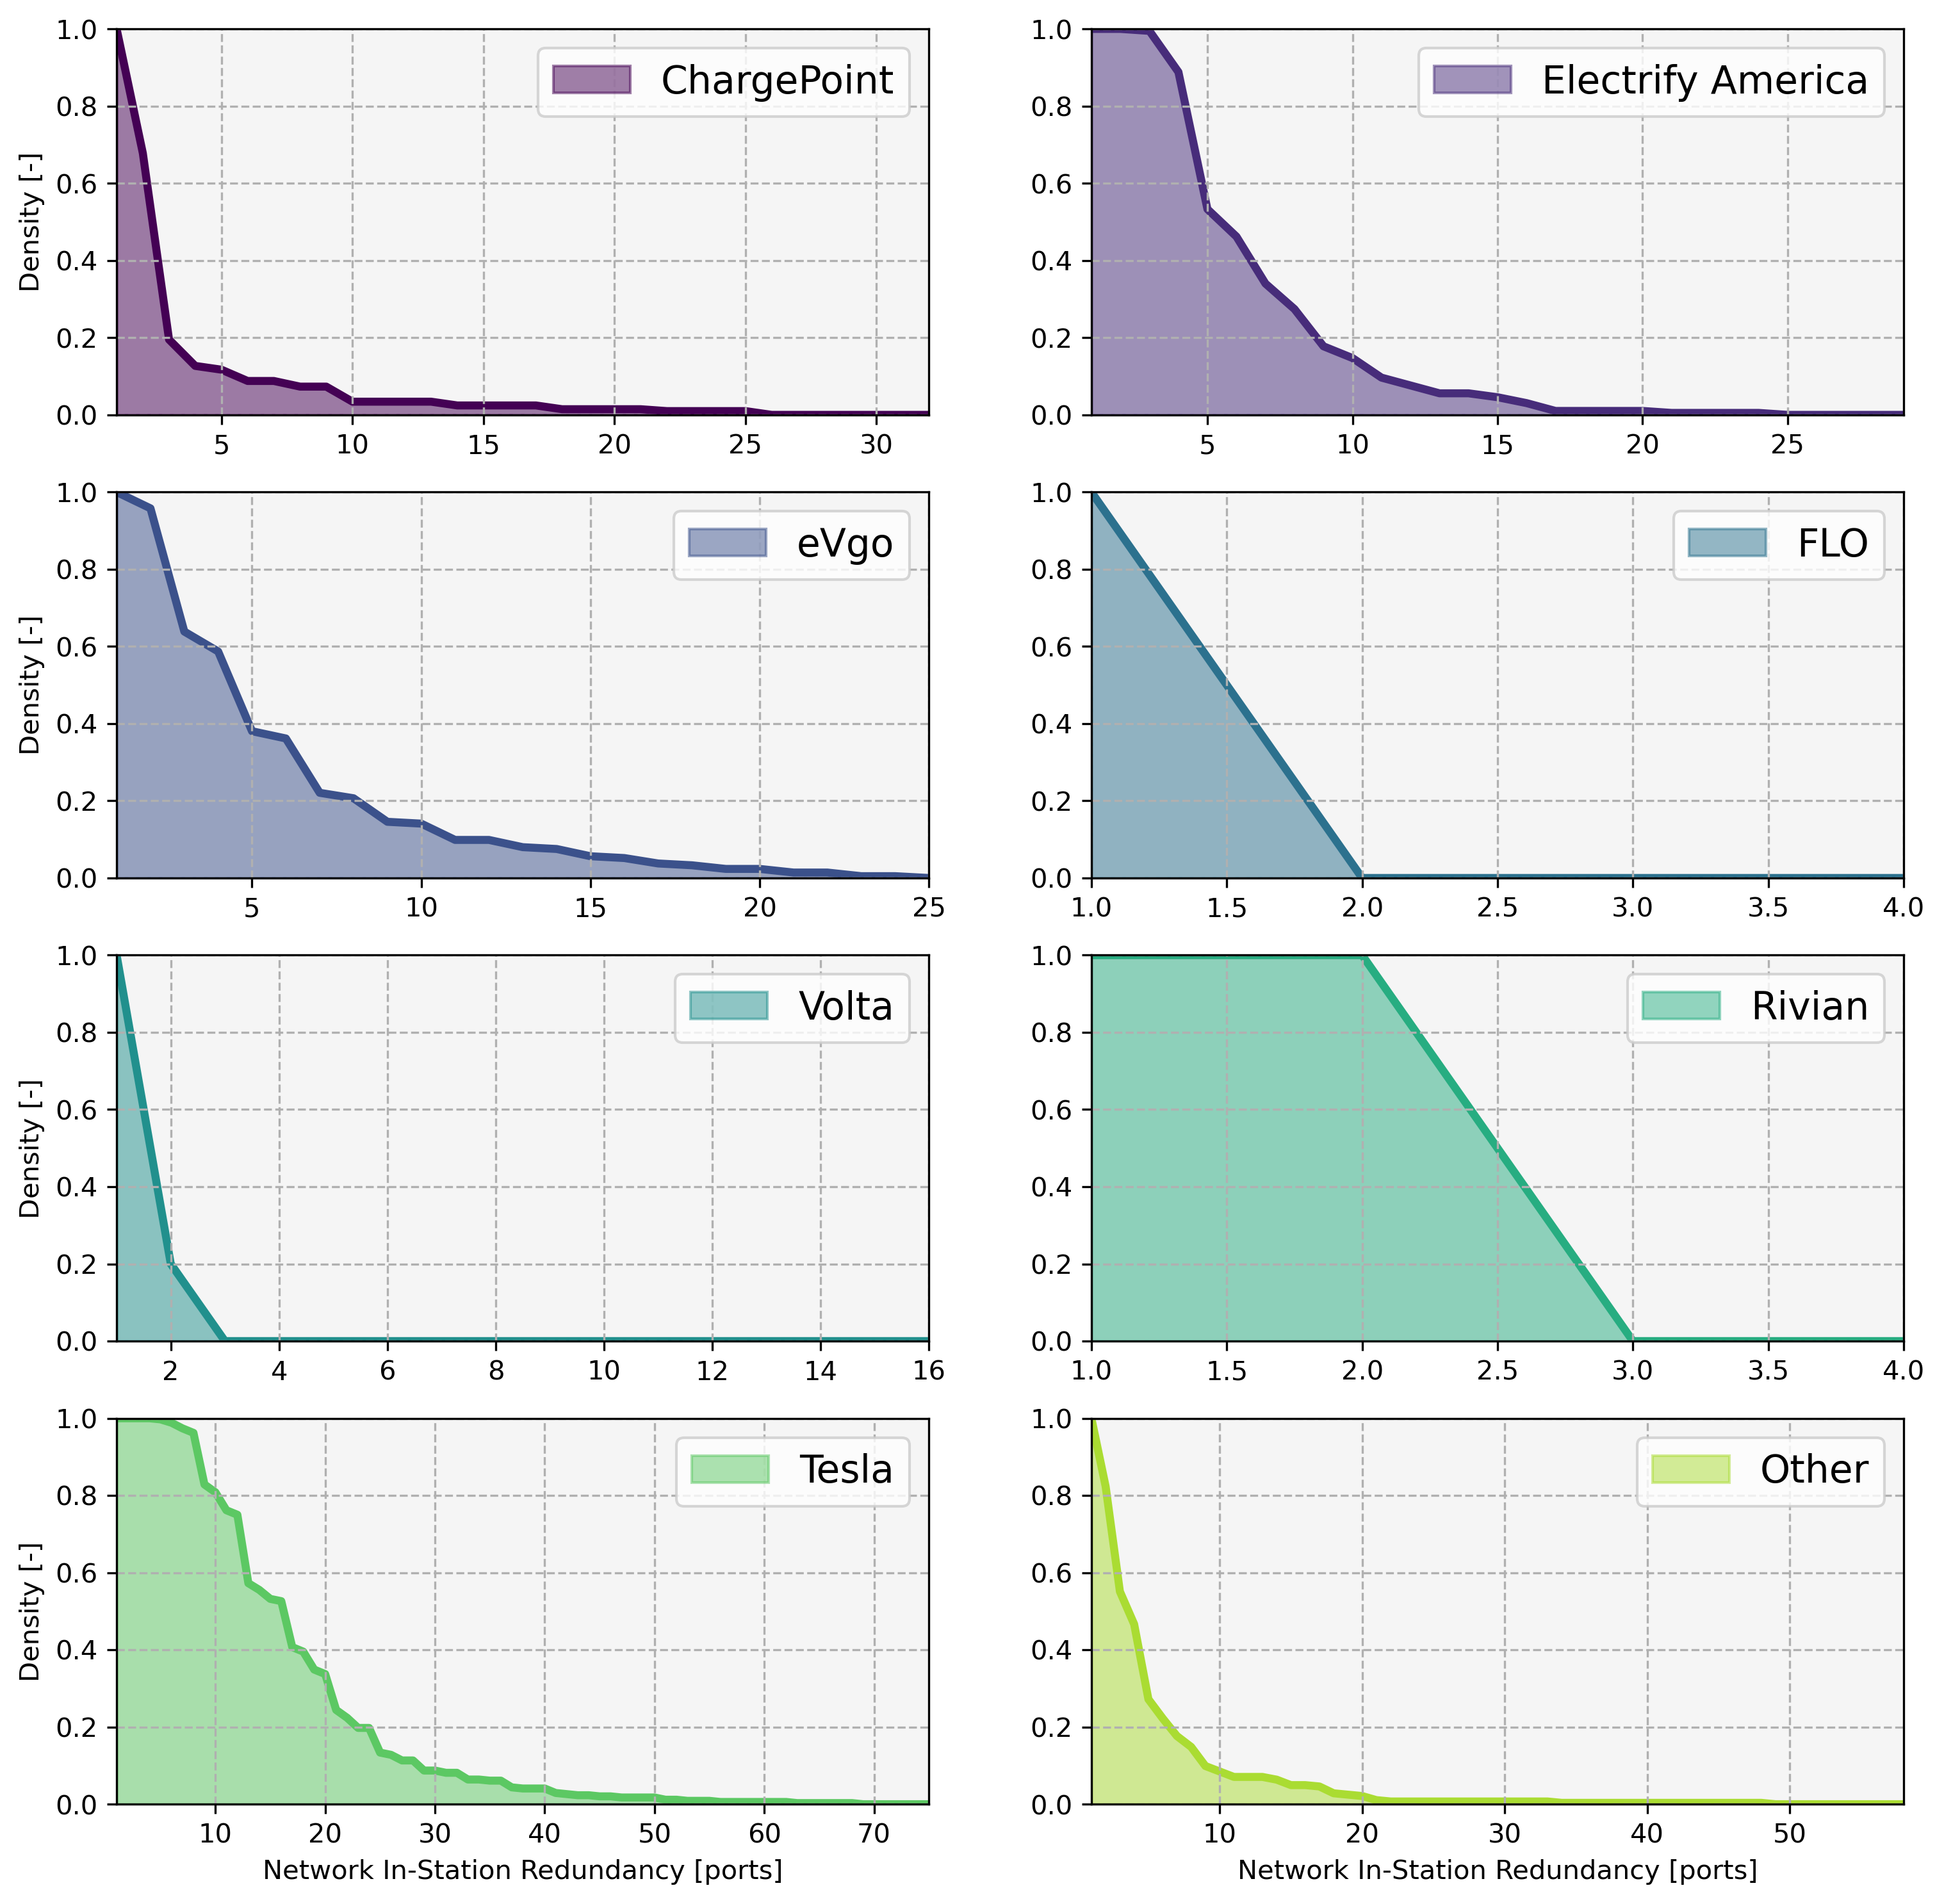
\includegraphics[width = \linewidth]{figs/California_RBS_600_SF_All.png}
%	\caption{In-station redundancy for DC Charging networks in California}
%	\label{fig:rbs_600_top_8_networks}
%\end{figure}

\begin{table}[H]
	\centering
	\caption{Summary statistics for California DC charging networks from \gls{afdc}}
	\label{tab:summary_statistics_afdc}
	\begin{tabular}{|C{.46\linewidth}|C{.18\linewidth}|C{.18\linewidth}|C{.18\linewidth}|}
		\hline Network & Chargers & Stations & Chargers per Station \\
		\hline Non-Networked & 260 & 123 & 2.1 \\
		\hline POWERFLEX & 43 & 11 & 3.9 \\
		\hline Blink Network & 30 & 12 & 2.5 \\
		\hline SHELL_RECHARGE & 84 & 34 & 2.5 \\
		\hline EV Connect & 122 & 47 & 2.6 \\
		\hline Tesla & 7093 & 418 & 17.0 \\
		\hline EVCS & 299 & 72 & 4.2 \\
		\hline Electrify America & 1152 & 243 & 4.7 \\
		\hline ChargePoint Network & 417 & 265 & 1.6 \\
		\hline Volta & 20 & 17 & 1.2 \\
		\hline EVGATEWAY & 118 & 22 & 5.4 \\
		\hline BP_PULSE & 49 & 14 & 3.5 \\
		\hline eVgo Network & 1367 & 339 & 4.0 \\
		\hline EVRANGE & 22 & 7 & 3.1 \\
		\hline RIVIAN_ADVENTURE & 30 & 15 & 2.0 \\
		\hline CHARGELAB & 1 & 1 & 1.0 \\
		\hline 7CHARGE & 25 & 8 & 3.1 \\
		\hline CIRCLE_K & 28 & 6 & 4.7 \\
		\hline LOOP & 13 & 5 & 2.6 \\
		\hline CHARGENET & 12 & 2 & 6.0 \\
		\hline NOODOE & 6 & 3 & 2.0 \\
		\hline
	\end{tabular}
\end{table}

\begin{table}[H]
	\centering
	\caption{Summary statistics for California DC charging networks from \gls{afdc} (corridor stations)}
	\label{tab:summary_statistics_afdc_corridor}
	\begin{tabular}{|C{.46\linewidth}|C{.18\linewidth}|C{.18\linewidth}|C{.18\linewidth}|}
		\hline Network & Chargers & Stations & Chargers per Station \\
		\hline Non-Networked & 258 & 50 & 5.2 \\
		\hline Tesla & 2471 & 142 & 17.4 \\
		\hline Electrify America & 468 & 68 & 6.9 \\
		\hline EV Connect & 66 & 19 & 3.5 \\
		\hline ChargePoint Network & 188 & 80 & 2.4 \\
		\hline EVCS & 37 & 11 & 3.4 \\
		\hline SHELL_RECHARGE & 41 & 11 & 3.7 \\
		\hline EVGATEWAY & 19 & 4 & 4.8 \\
		\hline BP_PULSE & 3 & 2 & 1.5 \\
		\hline eVgo Network & 311 & 58 & 5.4 \\
		\hline Blink Network & 1 & 1 & 1.0 \\
		\hline EVRANGE & 3 & 1 & 3.0 \\
		\hline RIVIAN_ADVENTURE & 10 & 5 & 2.0 \\
		\hline CIRCLE_K & 12 & 2 & 6.0 \\
		\hline 7CHARGE & 4 & 1 & 4.0 \\
		\hline LOOP & 2 & 1 & 2.0 \\
		\hline
	\end{tabular}
\end{table}

\begin{figure}[H]
	\centering
	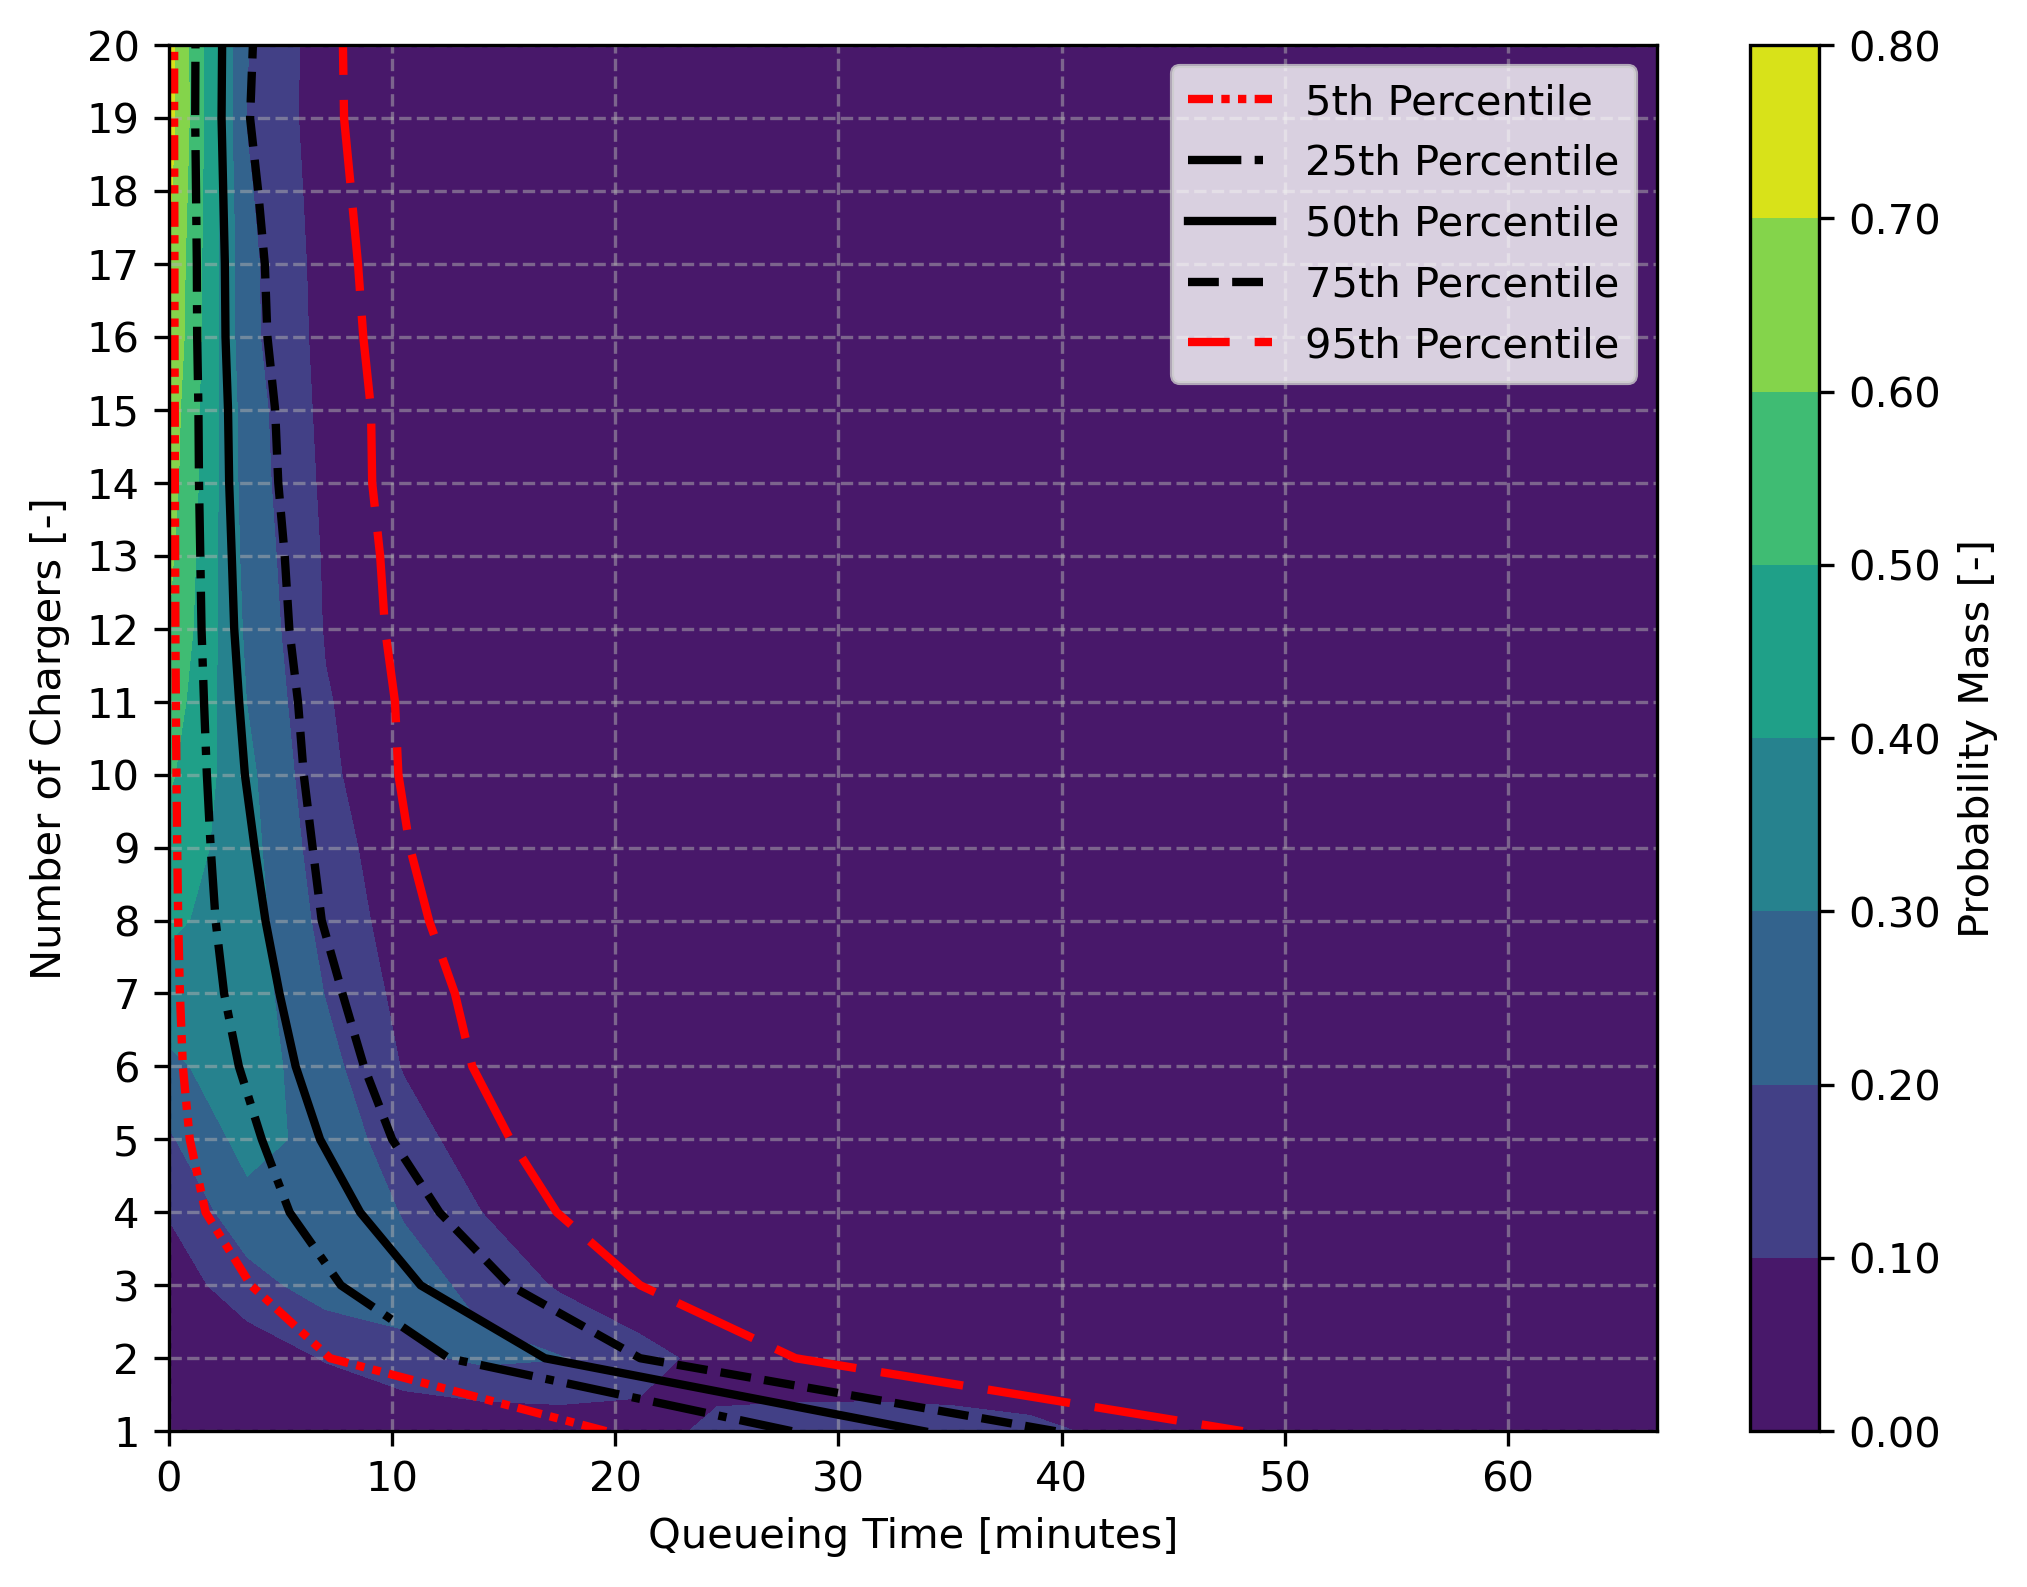
\includegraphics[width = \linewidth]{figs/expected_delay_contourf_1.png}
	\caption{PDFs of expected delay time for station with mean arrival ratio of 1, constant mean charge energy delivered of 45 kWh, and different in-station redundancy.}
	\label{fig:expected_delays_coutnours_1}
\end{figure}

\begin{figure}[H]
	\centering
	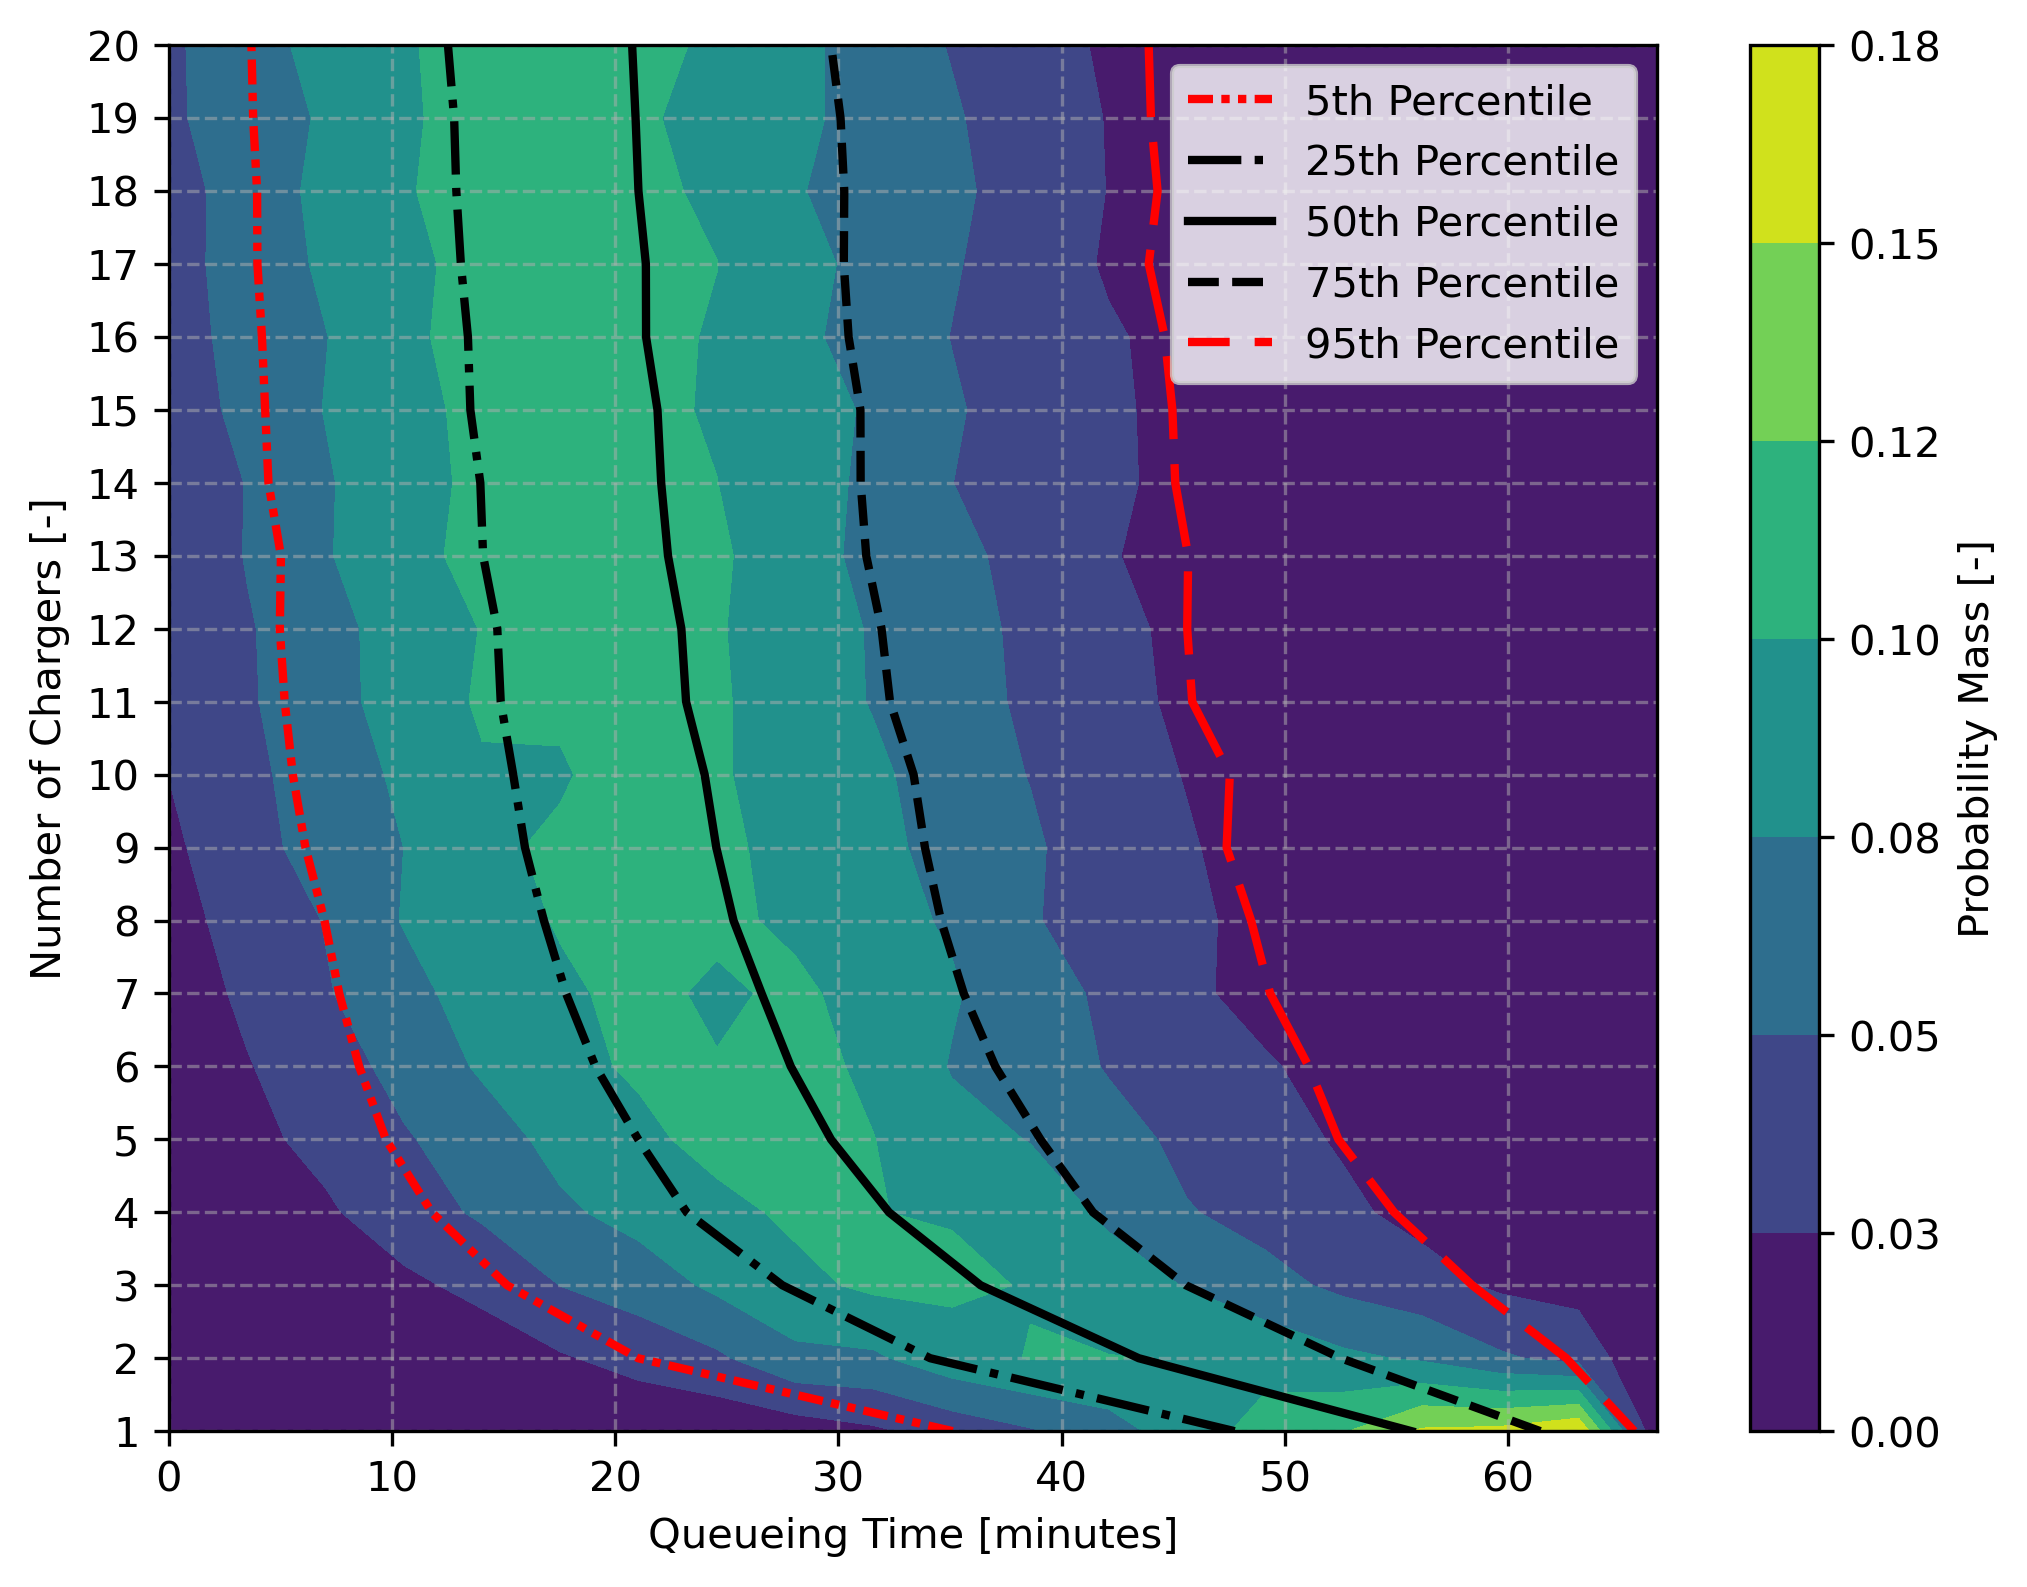
\includegraphics[width = \linewidth]{figs/expected_delay_contourf_2.png}
	\caption{PDFs of expected delay time for station with mean arrival ratio of 2, constant mean charge energy delivered of 45 kWh, and different in-station redundancy.}
	\label{fig:expected_delays_coutnours_2}
\end{figure}

\begin{figure}[H]
	\centering
	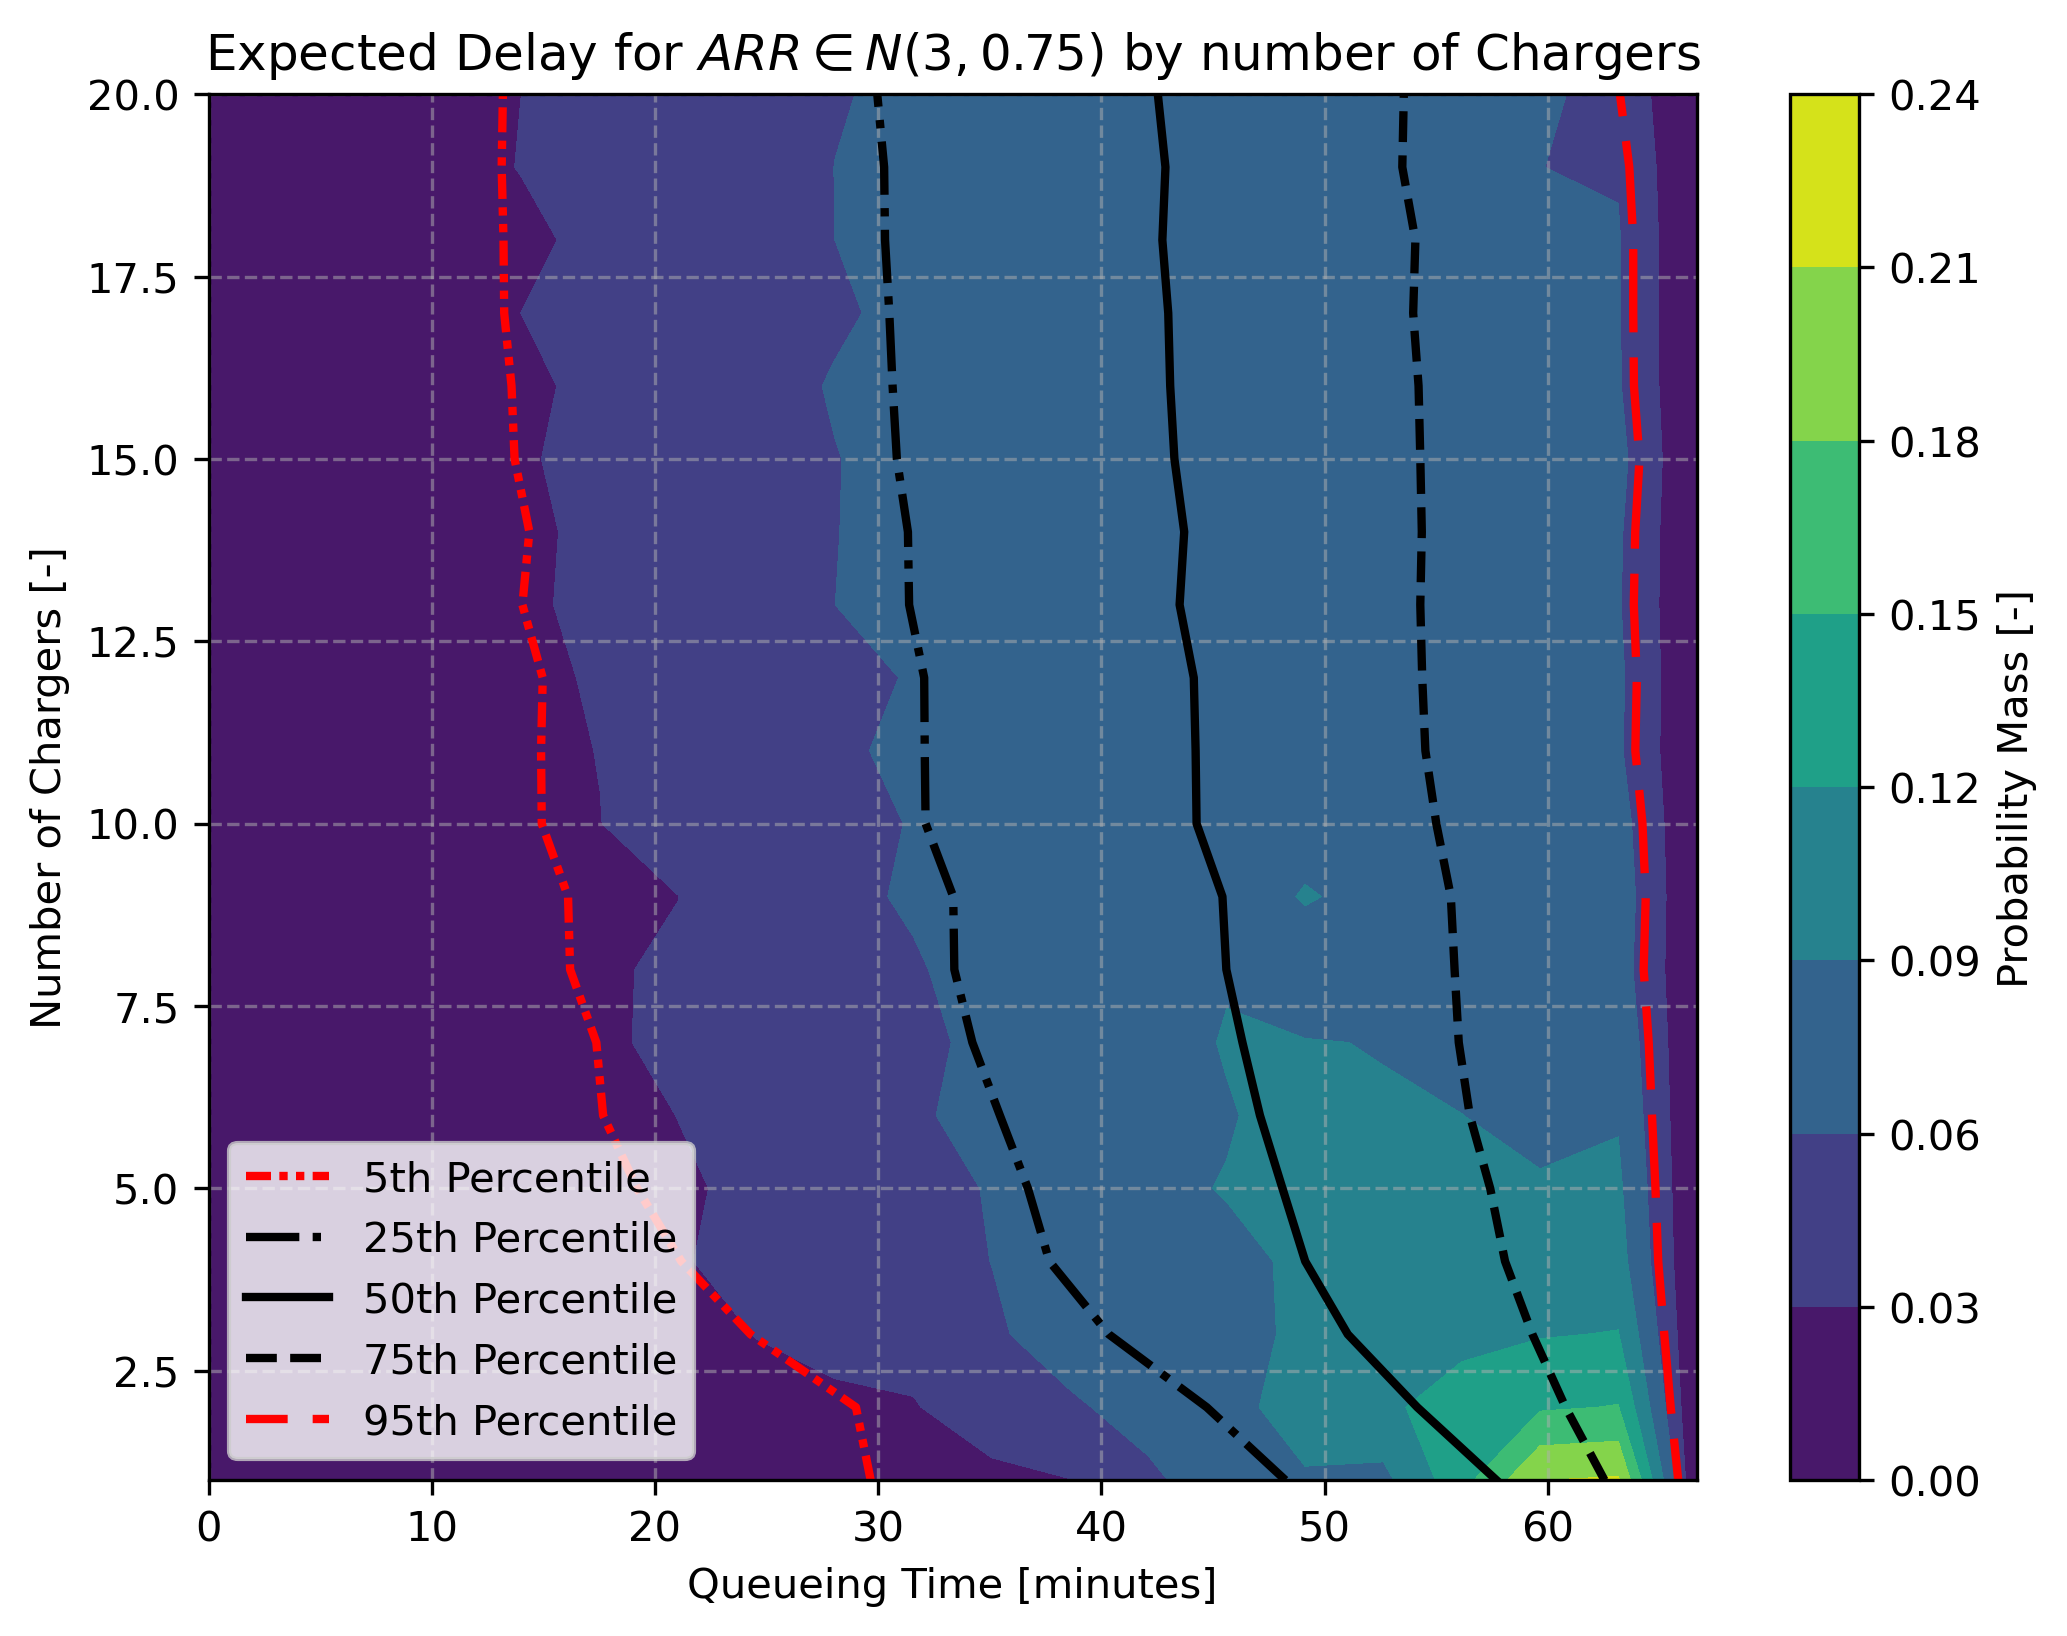
\includegraphics[width = \linewidth]{figs/expected_delay_contourf_3.png}
	\caption{PDFs of expected delay time for station with mean arrival ratio of 3, constant mean charge energy delivered of 45 kWh, and different in-station redundancy.}
	\label{fig:expected_delays_coutnours_3}
\end{figure}

\end{multicols}

\end{document}